% Options for packages loaded elsewhere
\PassOptionsToPackage{unicode}{hyperref}
\PassOptionsToPackage{hyphens}{url}
\PassOptionsToPackage{dvipsnames,svgnames,x11names}{xcolor}
%
\documentclass[
  letterpaper,
  DIV=11,
  numbers=noendperiod]{scrartcl}

\usepackage{amsmath,amssymb}
\usepackage{iftex}
\ifPDFTeX
  \usepackage[T1]{fontenc}
  \usepackage[utf8]{inputenc}
  \usepackage{textcomp} % provide euro and other symbols
\else % if luatex or xetex
  \usepackage{unicode-math}
  \defaultfontfeatures{Scale=MatchLowercase}
  \defaultfontfeatures[\rmfamily]{Ligatures=TeX,Scale=1}
\fi
\usepackage{lmodern}
\ifPDFTeX\else  
    % xetex/luatex font selection
\fi
% Use upquote if available, for straight quotes in verbatim environments
\IfFileExists{upquote.sty}{\usepackage{upquote}}{}
\IfFileExists{microtype.sty}{% use microtype if available
  \usepackage[]{microtype}
  \UseMicrotypeSet[protrusion]{basicmath} % disable protrusion for tt fonts
}{}
\makeatletter
\@ifundefined{KOMAClassName}{% if non-KOMA class
  \IfFileExists{parskip.sty}{%
    \usepackage{parskip}
  }{% else
    \setlength{\parindent}{0pt}
    \setlength{\parskip}{6pt plus 2pt minus 1pt}}
}{% if KOMA class
  \KOMAoptions{parskip=half}}
\makeatother
\usepackage{xcolor}
\setlength{\emergencystretch}{3em} % prevent overfull lines
\setcounter{secnumdepth}{5}
% Make \paragraph and \subparagraph free-standing
\ifx\paragraph\undefined\else
  \let\oldparagraph\paragraph
  \renewcommand{\paragraph}[1]{\oldparagraph{#1}\mbox{}}
\fi
\ifx\subparagraph\undefined\else
  \let\oldsubparagraph\subparagraph
  \renewcommand{\subparagraph}[1]{\oldsubparagraph{#1}\mbox{}}
\fi

\usepackage{color}
\usepackage{fancyvrb}
\newcommand{\VerbBar}{|}
\newcommand{\VERB}{\Verb[commandchars=\\\{\}]}
\DefineVerbatimEnvironment{Highlighting}{Verbatim}{commandchars=\\\{\}}
% Add ',fontsize=\small' for more characters per line
\usepackage{framed}
\definecolor{shadecolor}{RGB}{241,243,245}
\newenvironment{Shaded}{\begin{snugshade}}{\end{snugshade}}
\newcommand{\AlertTok}[1]{\textcolor[rgb]{0.68,0.00,0.00}{#1}}
\newcommand{\AnnotationTok}[1]{\textcolor[rgb]{0.37,0.37,0.37}{#1}}
\newcommand{\AttributeTok}[1]{\textcolor[rgb]{0.40,0.45,0.13}{#1}}
\newcommand{\BaseNTok}[1]{\textcolor[rgb]{0.68,0.00,0.00}{#1}}
\newcommand{\BuiltInTok}[1]{\textcolor[rgb]{0.00,0.23,0.31}{#1}}
\newcommand{\CharTok}[1]{\textcolor[rgb]{0.13,0.47,0.30}{#1}}
\newcommand{\CommentTok}[1]{\textcolor[rgb]{0.37,0.37,0.37}{#1}}
\newcommand{\CommentVarTok}[1]{\textcolor[rgb]{0.37,0.37,0.37}{\textit{#1}}}
\newcommand{\ConstantTok}[1]{\textcolor[rgb]{0.56,0.35,0.01}{#1}}
\newcommand{\ControlFlowTok}[1]{\textcolor[rgb]{0.00,0.23,0.31}{#1}}
\newcommand{\DataTypeTok}[1]{\textcolor[rgb]{0.68,0.00,0.00}{#1}}
\newcommand{\DecValTok}[1]{\textcolor[rgb]{0.68,0.00,0.00}{#1}}
\newcommand{\DocumentationTok}[1]{\textcolor[rgb]{0.37,0.37,0.37}{\textit{#1}}}
\newcommand{\ErrorTok}[1]{\textcolor[rgb]{0.68,0.00,0.00}{#1}}
\newcommand{\ExtensionTok}[1]{\textcolor[rgb]{0.00,0.23,0.31}{#1}}
\newcommand{\FloatTok}[1]{\textcolor[rgb]{0.68,0.00,0.00}{#1}}
\newcommand{\FunctionTok}[1]{\textcolor[rgb]{0.28,0.35,0.67}{#1}}
\newcommand{\ImportTok}[1]{\textcolor[rgb]{0.00,0.46,0.62}{#1}}
\newcommand{\InformationTok}[1]{\textcolor[rgb]{0.37,0.37,0.37}{#1}}
\newcommand{\KeywordTok}[1]{\textcolor[rgb]{0.00,0.23,0.31}{#1}}
\newcommand{\NormalTok}[1]{\textcolor[rgb]{0.00,0.23,0.31}{#1}}
\newcommand{\OperatorTok}[1]{\textcolor[rgb]{0.37,0.37,0.37}{#1}}
\newcommand{\OtherTok}[1]{\textcolor[rgb]{0.00,0.23,0.31}{#1}}
\newcommand{\PreprocessorTok}[1]{\textcolor[rgb]{0.68,0.00,0.00}{#1}}
\newcommand{\RegionMarkerTok}[1]{\textcolor[rgb]{0.00,0.23,0.31}{#1}}
\newcommand{\SpecialCharTok}[1]{\textcolor[rgb]{0.37,0.37,0.37}{#1}}
\newcommand{\SpecialStringTok}[1]{\textcolor[rgb]{0.13,0.47,0.30}{#1}}
\newcommand{\StringTok}[1]{\textcolor[rgb]{0.13,0.47,0.30}{#1}}
\newcommand{\VariableTok}[1]{\textcolor[rgb]{0.07,0.07,0.07}{#1}}
\newcommand{\VerbatimStringTok}[1]{\textcolor[rgb]{0.13,0.47,0.30}{#1}}
\newcommand{\WarningTok}[1]{\textcolor[rgb]{0.37,0.37,0.37}{\textit{#1}}}

\providecommand{\tightlist}{%
  \setlength{\itemsep}{0pt}\setlength{\parskip}{0pt}}\usepackage{longtable,booktabs,array}
\usepackage{calc} % for calculating minipage widths
% Correct order of tables after \paragraph or \subparagraph
\usepackage{etoolbox}
\makeatletter
\patchcmd\longtable{\par}{\if@noskipsec\mbox{}\fi\par}{}{}
\makeatother
% Allow footnotes in longtable head/foot
\IfFileExists{footnotehyper.sty}{\usepackage{footnotehyper}}{\usepackage{footnote}}
\makesavenoteenv{longtable}
\usepackage{graphicx}
\makeatletter
\def\maxwidth{\ifdim\Gin@nat@width>\linewidth\linewidth\else\Gin@nat@width\fi}
\def\maxheight{\ifdim\Gin@nat@height>\textheight\textheight\else\Gin@nat@height\fi}
\makeatother
% Scale images if necessary, so that they will not overflow the page
% margins by default, and it is still possible to overwrite the defaults
% using explicit options in \includegraphics[width, height, ...]{}
\setkeys{Gin}{width=\maxwidth,height=\maxheight,keepaspectratio}
% Set default figure placement to htbp
\makeatletter
\def\fps@figure{htbp}
\makeatother

\KOMAoption{captions}{tableheading}
\makeatletter
\@ifpackageloaded{caption}{}{\usepackage{caption}}
\AtBeginDocument{%
\ifdefined\contentsname
  \renewcommand*\contentsname{Table of contents}
\else
  \newcommand\contentsname{Table of contents}
\fi
\ifdefined\listfigurename
  \renewcommand*\listfigurename{List of Figures}
\else
  \newcommand\listfigurename{List of Figures}
\fi
\ifdefined\listtablename
  \renewcommand*\listtablename{List of Tables}
\else
  \newcommand\listtablename{List of Tables}
\fi
\ifdefined\figurename
  \renewcommand*\figurename{Figure}
\else
  \newcommand\figurename{Figure}
\fi
\ifdefined\tablename
  \renewcommand*\tablename{Table}
\else
  \newcommand\tablename{Table}
\fi
}
\@ifpackageloaded{float}{}{\usepackage{float}}
\floatstyle{ruled}
\@ifundefined{c@chapter}{\newfloat{codelisting}{h}{lop}}{\newfloat{codelisting}{h}{lop}[chapter]}
\floatname{codelisting}{Stan

Program}
\newcommand*\listoflistings{\listof{codelisting}{List of Listings}}
\makeatother
\makeatletter
\makeatother
\makeatletter
\@ifpackageloaded{caption}{}{\usepackage{caption}}
\@ifpackageloaded{subcaption}{}{\usepackage{subcaption}}
\makeatother
\ifLuaTeX
  \usepackage{selnolig}  % disable illegal ligatures
\fi
\usepackage{bookmark}

\IfFileExists{xurl.sty}{\usepackage{xurl}}{} % add URL line breaks if available
\urlstyle{same} % disable monospaced font for URLs
\hypersetup{
  pdftitle={Mixture Modeling},
  pdfauthor={Michael Betancourt},
  colorlinks=true,
  linkcolor={blue},
  filecolor={Maroon},
  citecolor={Blue},
  urlcolor={Blue},
  pdfcreator={LaTeX via pandoc}}

\title{Mixture Modeling}
\author{Michael Betancourt}
\date{October 2024}

\begin{document}
\maketitle

\renewcommand*\contentsname{Table of contents}
{
\hypersetup{linkcolor=}
\setcounter{tocdepth}{3}
\tableofcontents
}
Sometimes a single data generating process just isn't enough. When
observations can arise from multiple data generating processes we need
to model each of those data generating processes. If we don't know which
of those possible data generating processes is responsible for a
particular observation then we need to appeal to \emph{mixture
modeling}.

Mixture modeling allows us to, for example, account for undesired
contamination, such as an irreducible background that overlaps with a
desired signal. By mixing together probabilistic models for the signal
and background events we can learn not only the behavior of each but
also their relative prevalence in the observed data.

In this chapter we'll review the mathematical foundations and general
implementation of mixture models, including the potential for
frustrating inferential behaviors. Finally we'll illustrate these ideas
with a series of demonstrative analyses.

\section{Implementing Mixture Models}\label{implementing-mixture-models}

From a mathematical perspective mixing multiple data generating
processes together is relatively straightforward. We have to do a bit of
work, however, to derive an implementation that performs well in
practice.

\subsection{Categorical Implementations}\label{sec:cat_impl}

Consider an observational space \(Y\) and a collection of \(K\)
component probability distributions specified with the probability
density functions, \(p_{k}(y)\), each modeling a distinct data
generating process. To simplify the initial presentation we will assume
that each component probability distribution is fixed so that there no
model configuration variables to consider.

The most straightforward way to model an observation that can arise from
any of these components is to introduce a categorical variable that
labels the responsible data generating process, \[
z \in \{ 1, \ldots, k, \ldots, K \},
\] and a corresponding probabilistic model \[
p(z = k \mid \lambda_{1}, \ldots, \lambda_{K}) = \lambda_{k}
\] where the \(\lambda_{k}\) from a simplex, \begin{align*}
0 \le \lambda_{k} &\le 1
\\
\sum_{k = 1}^{K} \lambda_{k} &= 1.
\end{align*}

Each observation is then modeled with a value \(y \in Y\), an assignment
\(z\), and the full Bayesian model \begin{align*}
p(y, z \mid \lambda_{1}, \ldots, \lambda_{K})
&=
p(y \mid z) \, p(z \mid \lambda_{1}, \ldots, \lambda_{K})
\\
&=
p_{z}(y) \, \lambda_{z}.
\end{align*}

If we know the responsible data generating process then the component
assignment variable \(z\) will be observed along with \(y\), but if we
do not know \(z\) then all we can do is infer it from the observed value
of \(y\). Assuming that the component probabilities and probability
distributions are known the consistent component assignment are given by
an application of Bayes' Theorem, \begin{align*}
p(z \mid \tilde{y}, \lambda_{1}, \ldots, \lambda_{K})
&=
\frac{
  p(\tilde{y}, z \mid \lambda_{1}, \ldots, \lambda_{K})
}{
  \sum_{k = 1}^{K} p(\tilde{y}, k \mid \lambda_{1}, \ldots, \lambda_{K})
}
\\
&=
\frac{ p_{z}(\tilde{y}) \, \lambda_{z}}
{ \sum_{k = 1}^{K} p_{k}(\tilde{y}) \, \lambda_{k} }.
\end{align*}

When modeling multiple, independent observations from overlapping data
generating processes we have to consider the heterogeneity of the
categorical variables. In particular if all of the categorical variables
are modeled with the same component probabilities then the joint full
Bayesian model becomes \begin{align*}
p(y_{1}, z_{1}, \ldots, y_{N}, z_{N} \mid
  \lambda_{1}, \ldots, \lambda_{K})
&=
\prod_{n = 1}^{N}
p(y_{n} \mid z_{n}) \, p(z_{n} \mid \lambda_{1}, \ldots, \lambda_{K})
\\
&=
p_{z_{n}}(y_{n}) \, \lambda_{z_{n}}.
\end{align*} On the other hand if the component probabilities can vary
across observations then we need a separate simplex for each
observation, \[
\boldsymbol{\lambda}_{n} = ( \lambda_{n, 1}, \ldots, \lambda_{n, K}),
\] and the joint full Bayesian model becomes \begin{align*}
p(y_{1}, z_{1}, \ldots, y_{N}, z_{N} \mid
  \boldsymbol{\lambda}_{1}, \ldots, \boldsymbol{\lambda}_{N})
&=
\prod_{n = 1}^{N}
p(y_{n} \mid z_{n}) \, p(z_{n} \mid \boldsymbol{\lambda}_{n})
\\
&=
p_{z_{n}}(y_{n}) \, \lambda_{n, z_{n}}.
\end{align*}

In either case inferences of the individual \(z_{n}\) depend on only the
observed \(y_{n}\), \[
p(z_{n} \mid \tilde{y}_{n}, \lambda_{1}, \ldots, \lambda_{K})
=
\frac{ p_{z_{n}}(\tilde{y}_{n}) \, \lambda_{z_{n}}}
{ \sum_{k = 1}^{K} p_{k}(\tilde{y}_{n}) \, \lambda_{k} },
\] again conditioned on the component probabilities and component
probability distributions.

\subsection{Marginal Implementations}\label{marginal-implementations}

In practice unknown categorical variables can quickly become a nuisance.
Not only do they introduce a new variable that we have to infer for each
observation but also those variables are discrete which limits the
available computational tools. Specifically we cannot use gradient-based
methods like Hamiltonian Monte Carlo to explore posterior distributions
over the component assignments and component probabilities, let alone
the configuration of the component probability distributions.

Fortunately marginalizing unknown categorical assignments out of the
full Bayesian model is straightforward.

\subsubsection{Single Observation}\label{single-observation}

For a single observation marginalizing an unknown component assignment
requires summing over the \(K\) possible values, \begin{align*}
p(y \mid \lambda_{1}, \ldots, \lambda_{K})
&=
\sum_{k = 1}^{K}
p(y, z = k \mid \lambda_{1}, \ldots, \lambda_{K})
\\
&=
\sum_{k = 1}^{K}
p(y \mid z = k) \, p(z = k \mid \lambda_{1}, \ldots, \lambda_{K})
\\
&=
\sum_{k = 1}^{K}
p_{k}(y) \, \lambda_{k}.
\end{align*} In other words all we have to do eliminate an categorical
variable is add together all of the the component probability density
functions weighted by the component probabilities.

\subsubsection{Multiple Homogeneous
Observations}\label{multiple-homogeneous-observations}

Given multiple, independent observations modeled by the same component
probabilities we can marginalize each component individually,
\begin{align*}
p(y_{1}, \ldots, y_{N} \mid \lambda_{1}, \ldots, \lambda_{K})
&=
\prod_{n = 1}^{N} p(y_{n} \mid \lambda_{1}, \ldots, \lambda_{K})
\\
&=
\prod_{n = 1}^{N} \sum_{k = 1}^{K} p_{k}(y_{n}) \, \lambda_{k}.
\end{align*}

\subsubsection{Multiple Heterogeneous
Observations}\label{multiple-heterogeneous-observations}

Accounting for heterogeneity in the component probabilities is a bit
more cumbersome, \begin{align*}
p(y_{1}, \ldots, y_{N} \mid
  \boldsymbol{\lambda}_{1}, \ldots, \boldsymbol{\lambda}_{N})
&=
\prod_{n = 1}^{N} p(y_{n} \mid \boldsymbol{\lambda}_{n})
\\
&=
\prod_{n = 1}^{N} \sum_{k = 1}^{K} p_{k}(y_{n}) \, \lambda_{n, k}.
\end{align*}

Interesting we can sometimes simplify the heterogeneous model even
further by marginalizing out not only the individual categorical
variables but also the individual simplices! Specifically we need the
individual simplices to be independent and identically distributed so
that any consistent probabilistic model is of the form \[
p(\boldsymbol{\lambda}_{n}, \ldots, \boldsymbol{\lambda}_{n})
=
\prod_{n = 1}^{N} p(\boldsymbol{\lambda}_{n}).
\]

In this case the expectation value of any component probability is the
same for all observations, \begin{align*}
\int \mathrm{d} \boldsymbol{\lambda}_{1} \cdots
     \mathrm{d} \boldsymbol{\lambda}_{N}
p(\boldsymbol{\lambda}_{1}, \ldots, \boldsymbol{\lambda}_{N}) \,
\lambda_{n, k}
&=
\int \mathrm{d} \boldsymbol{\lambda}_{1} \cdots
     \mathrm{d} \boldsymbol{\lambda}_{N}
\bigg[ \prod_{n = 1}^{N} p(\boldsymbol{\lambda}_{n}) \bigg] \,
\lambda_{n, k}
\\
&=
\prod_{n' \ne 1}^{N}
\int \mathrm{d} \boldsymbol{\lambda}_{n'}
p(\boldsymbol{\lambda}_{n})
\cdot
\int \mathrm{d} \boldsymbol{\lambda}_{n} \,
p(\boldsymbol{\lambda}_{n}) \, \lambda_{n, k}
\\
&=
\prod_{n' \ne 1}^{N} 1 \cdot
\int \mathrm{d} \boldsymbol{\lambda}_{n} \,
p(\boldsymbol{\lambda}_{n}) \, \lambda_{n, k}
\\
&=
\int \mathrm{d} \boldsymbol{\lambda}_{n} \,
p(\boldsymbol{\lambda}_{n}) \, \lambda_{n, k}
\\
&\equiv
\omega_{k}.
\end{align*}

Moreover these individual expectation values form their own simplex: the
boundedness of each \(\lambda_{n, k}\) implies that \[
0 \le \omega_{k} \le 1
\] while \begin{align*}
\sum_{k = 1}^{K} \omega_{k}
&=
\sum_{k = 1}^{K}
\int \mathrm{d} \boldsymbol{\lambda}_{n} \,
p(\boldsymbol{\lambda}_{n}) \, \lambda_{n, k}
\\
&=
\int \mathrm{d} \boldsymbol{\lambda}_{n} \,
p(\boldsymbol{\lambda}_{n}) \, \sum_{k = 1}^{K} \lambda_{n, k}
\\
&=
\int \mathrm{d} \boldsymbol{\lambda}_{n} \,
p(\boldsymbol{\lambda}_{n}) \, 1
\\
&=
1.
\end{align*}

Under these assumptions the marginal mixture model is given by
\begin{align*}
p(y_{1}, \ldots, y_{N})
&=
\int \mathrm{d} \boldsymbol{\lambda}_{1} \cdots
     \mathrm{d} \boldsymbol{\lambda}_{N}
p(y_{1}, \ldots, y_{N},
  \boldsymbol{\lambda}_{1}, \ldots, \boldsymbol{\lambda}_{N})
\\
&=
\int \mathrm{d} \boldsymbol{\lambda}_{1} \cdots
     \mathrm{d} \boldsymbol{\lambda}_{N}
\bigg[
\prod_{n = 1}^{N} \sum_{k = 1}^{K} p_{k}(y_{n}) \, \lambda_{n, k}
\bigg]
\prod_{n = 1}^{N} p(\boldsymbol{\lambda}_{n})
\\
&=
\prod_{n = 1}^{N}
\int \mathrm{d} \boldsymbol{\lambda}_{n}
\bigg[
\sum_{k = 1}^{K} p_{k}(y_{n}) \, \lambda_{n, k}
\bigg]
p(\boldsymbol{\lambda}_{n})
\\
&=
\prod_{n = 1}^{N}
\sum_{k = 1}^{K} \bigg[ p_{k}(y_{n})
\int \mathrm{d} \boldsymbol{\lambda}_{n} \,
p(\boldsymbol{\lambda}_{n}) \, \lambda_{n, k} \bigg]
\\
&=
\prod_{n = 1}^{N}
\sum_{k = 1}^{K} \bigg[ p_{k}(y_{n}) \, \omega_{k} \bigg].
\end{align*}

In other words the heterogeneous model reduces to the same form as the
homogeneous mixture model only with a new simplex \[
\boldsymbol{\omega} = (\omega_{1}, \ldots, \omega_{K})!
\] The new simplex components \(\omega_{k}\) can no longer be
interpreted as the probability of any \emph{individual} observation
arising from a particular component data generating process. Instead
they capture the \emph{proportion} of the ensemble of observations that
arises from each component data generating process.

\subsection{Numerically Stable Marginal
Implementations}\label{sec:stable_impl}

Most probabilistic programming languages, for example the Stan modeling
language, work not with probability density functions \(p(y)\) but
rather log probability density functions \(\log \circ \, p(y)\).
Consequently in order to implement a mixture model in these languages we
need to evaluate \begin{align*}
\log \circ \, p(y_{1}, \ldots, y_{N} \mid \lambda_{1}, \ldots, \lambda_{K})
&=
\log \bigg(
\prod_{n = 1}^{N} \sum_{k = 1}^{K} \lambda_{k} p_{k}(y_{n})
\bigg)
\\
&=
\sum_{n = 1}^{N}
\log \bigg( \sum_{k = 1}^{K} \lambda_{k} p_{k}(y_{n}) \bigg)
\\
&=
\sum_{n = 1}^{N}
\log \bigg(
\sum_{k = 1}^{K} \lambda_{k} \exp( \log \circ \, p_{k}(y_{n}) )
\bigg)
\\
&=
\sum_{n = 1}^{N}
\log \bigg(
\sum_{k = 1}^{K} \exp( \log(\lambda_{k}) + \log \circ \, p_{k}(y_{n}) ).
\bigg)
\end{align*} In other words for each observation we need to exponentiate
a term for each component, evaluate the sum of the exponentials, and
then apply the natural logarithm function again.

This composite operation is often referred to as the ``log sum exp''
function, \[
\text{log-sum-exp}(x_{1}, \ldots, x_{K})
=
\log \bigg( \sum_{k = 1}^{K} \exp (x_{k}) \bigg).
\] Implementing this operation on computers is complicated by the
limitations of floating point arithmetic. In particular the intermediate
terms \(\exp(x_{k})\) are prone to overflowing to floating point
infinity and corrupting the calculation before the final logarithm can
calm things down.

That said the properties of logarithms and exponentials allow us to
implement the log sum exp operation in a variety of ways. Specifically
we can always factor out any one component without affecting the final
value, \begin{align*}
\text{log-sum-exp}(x_{1}, \ldots, x_{K})
&=
\log \bigg( \sum_{k = 1}^{K} \exp (x_{k}) \bigg)
\\
&=
\log \bigg( \exp (x_{k'}) + \sum_{k \ne k'} \exp (x_{k}) \bigg)
\\
&=
\log \bigg( \exp (x_{k'}) \bigg)
\bigg(1 + \sum_{k \ne k'} \frac{ \exp (x_{k}) }{ \exp (x_{k'}) } \bigg)
\\
&=
\log \bigg( \exp (x_{k'}) \bigg)
\bigg(1 + \sum_{k \ne k'} \exp (x_{k} - x_{k'}) \bigg)
\\
&=
\log \exp (x_{k'})
+ \log \bigg(1 + \sum_{k \ne k'} \exp (x_{k} - x_{k'}) \bigg)
\\
&=
x_{k'} + \log \bigg(1 + \sum_{k \ne k'} \exp (x_{k} - x_{k'}) \bigg).
\end{align*}

If we factor out the largest component value then \[
x_{k'} \ge x_{k \ne k'}
\] and the input to each exponential will always be less than or equal
to one and the calculation will never encounter floating point overflow.
Conveniently most computational libraries provide log sum exp function
implementations that automatically factor out the largest value and
ensure stable numerical computation. Consequently we need to worry about
numerical stability only when implementing operations like these
ourselves.

For example in Stan we can avoid any issues by using the built-in
\texttt{log\_sum\_exp} function.

\begin{Shaded}
\begin{Highlighting}[]
\CommentTok{// Loop over observations}
\ControlFlowTok{for}\NormalTok{ (n }\ControlFlowTok{in} \DecValTok{1}\NormalTok{:N) \{}
  \KeywordTok{target +=}\NormalTok{ log\_sum\_exp(log(lambda[}\DecValTok{1}\NormalTok{]) + foo1\_lpdf(y[n]),}
\NormalTok{                        log(lambda[}\DecValTok{2}\NormalTok{]) + foo2\_lpdf(y[n]),}
\NormalTok{                        log(lambda[}\DecValTok{3}\NormalTok{]) + foo3\_lpdf(y[n]),}
\NormalTok{                        log(lambda[}\DecValTok{4}\NormalTok{]) + foo4\_lpdf(y[n]));}
\NormalTok{\}}
\end{Highlighting}
\end{Shaded}

Conveniently this function is also vectorized so we can call it with a
single vector argument.

\begin{Shaded}
\begin{Highlighting}[]
\CommentTok{// Loop over observations}
\ControlFlowTok{for}\NormalTok{ (n }\ControlFlowTok{in} \DecValTok{1}\NormalTok{:N) \{}
  \DataTypeTok{vector}\NormalTok{[}\DecValTok{4}\NormalTok{] lpds = [ foo1\_lpdf(y[n]), foo2\_lpdf(y[n]),}
\NormalTok{                     foo3\_lpdf(y[n]), foo4\_lpdf(y[n]) ]\textquotesingle{};}
  \KeywordTok{target +=}\NormalTok{ log\_sum\_exp(log(lambda) + lpds);}
\NormalTok{\}}
\end{Highlighting}
\end{Shaded}

When working with only two components there is also a \texttt{log\_mix}
function that incorporates the mixture probabilities directly.

\begin{Shaded}
\begin{Highlighting}[]
\NormalTok{log\_mix(theta, foo1\_lpdf(y[n]), foo2\_lpdf(y[n]))}
\NormalTok{=}
\NormalTok{log\_sum\_exp(log(theta)     + foo1\_lpdf(y[n]),}
\NormalTok{            log(}\DecValTok{1}\NormalTok{ {-} theta) + foo2\_lpdf(y[n]))}
\end{Highlighting}
\end{Shaded}

All of this said there is one additional numerical concern relevant to
the implementation of mixture models. If any categorical probability
vanishes, \[
\lambda_{k} = 0,
\] then the input to the log sum exp function will overflow to negative
infinity, \begin{align*}
x_{k'}
&=
\log(\lambda_{k'}) + \log \circ \, p_{k'}(y)
\\
&=
-\infty + \log \circ \, p_{k'}(y)
\\
&=
-\infty.
\end{align*} At the same time negative infinities also arise if any of
the component probability density functions vanish, \begin{align*}
x_{k'}
&=
\log(\lambda_{k'}) + \log \circ \, p_{k'}(y)
\\
&=
\log(\lambda_{k'}) + \log(0)
\\
&=
\log(\lambda_{k'}) -\infty
\\
&=
-\infty.
\end{align*}

Formally any negative infinite input results in a vanishing exponential
output \[
exp(x_{k}) = exp(-\infty) = 0
\] and no contribution to the intermediate sum. \[
\sum_{k = 1}^{K} \exp(x_{k}) = \sum_{k \ne k'} \exp (x_{k}),
\] Consequently we have, at least in theory, the identity \begin{align*}
\text{log-sum-exp}&(x_{1}, \ldots, x_{k - 1}, x_{k} = -\infty,
                     x_{k + 1}, \ldots, x_{K})
\\
&=
\text{log-sum-exp}(x_{1}, \ldots, x_{k - 1},
                     x_{k + 1}, \ldots, x_{K}).
\end{align*} In practice, however, the negative infinity can wreak havoc
on the floating point calculations.

To avoid potential numerical complications entirely we need to drop the
offending component \emph{before} trying to evaluate the inputs to the
log sum exp function. Specifically we compute \[
x_{k} = \log(\lambda_{k}) + p_{k}(y)
\] for only the components with \(\lambda_{k} > 0\) and
\(p_{k}(y) > 0\), and then evaluate the log sum exp function on only
these well-behaved inputs.

\subsection{Sampling From Mixture Models}\label{sec:sampling}

Although we've done a good bit of work to remove the component
assignments from mixture models they are not without their uses. Indeed
they make sampling from a mixture model particularly straightforward.

The unmarginalized full Bayesian model \[
p(y, z \mid \lambda_{1}, \ldots, \lambda_{K})
=
p(y \mid z) \, p(z \mid \lambda_{1}, \ldots, \lambda_{K})
\] immediately motivates an ancestral sampling strategy. We first select
a component by sampling a categorical variable
(Figure~\ref{fig-sampling-one}) \[
\tilde{z} \sim p(z \mid \lambda_{1}, \ldots, \lambda_{K})
\] and then sample from the corresponding component probability
distribution (Figure~\ref{fig-sampling-two}) \[
\tilde{y} \sim p(y \mid \tilde{z}) = p_{\tilde{z}}(y).
\]

\begin{figure}

\begin{minipage}{0.05\linewidth}
~\end{minipage}%
%
\begin{minipage}{0.45\linewidth}

\centering{

\captionsetup{labelsep=none}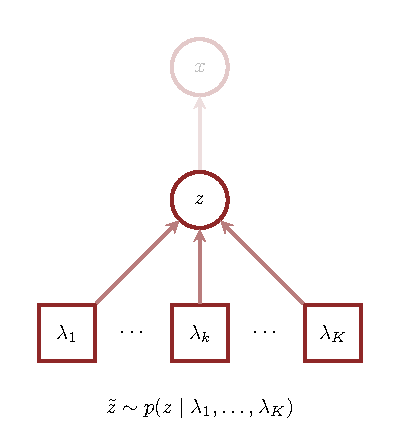
\includegraphics{figures/sampling/one/one.pdf}

}

\subcaption{\label{fig-sampling-one}}

\end{minipage}%
%
\begin{minipage}{0.45\linewidth}

\centering{

\captionsetup{labelsep=none}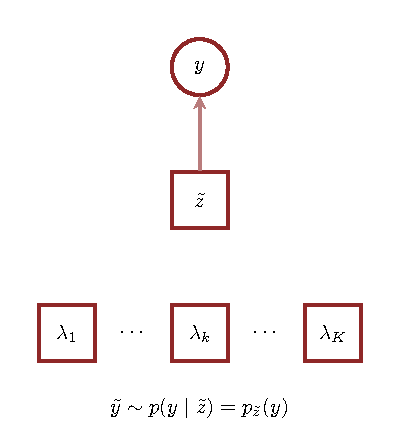
\includegraphics{figures/sampling/two/two.pdf}

}

\subcaption{\label{fig-sampling-two}}

\end{minipage}%

\caption{\label{fig-sampling}Sampling from a mixture model is a
straightforward, two-step process. (a) We first sample a component
\(\tilde{z}\) given the component probabilities
\(p(z = k) = \lambda_{k}\) and then (b) sample an observation
\(\tilde{y}\) from the corresponding component probability distribution
\(p_{\tilde{z}}(y)\).}

\end{figure}%

Together the pair \(\{ \tilde{y}, \tilde{z} \}\) defines a sample from
the unmarginalized model, \[
\{ \tilde{y}, \tilde{z} \}
\sim
p(y, z \mid \lambda_{1}, \ldots, \lambda_{K}),
\] while the single value \(\tilde{y}\) defines a sample from the
marginalized model, \[
\tilde{y} \sim p(y \mid \lambda_{1}, \ldots, \lambda_{K}).
\]

Implementing this two-step sampling procedure in the Stan Modeling
Language is straightforward.

\begin{Shaded}
\begin{Highlighting}[]
\CommentTok{// Loop over observations}
\ControlFlowTok{for}\NormalTok{ (n }\ControlFlowTok{in} \DecValTok{1}\NormalTok{:N) \{}
  \CommentTok{// Sample a component}
  \DataTypeTok{int}\NormalTok{\textless{}}\KeywordTok{lower}\NormalTok{=}\DecValTok{1}\NormalTok{, }\KeywordTok{upper}\NormalTok{=K\textgreater{} z = categorical\_rng(lambda);}
  \CommentTok{// Sample an observation}
  \ControlFlowTok{if}\NormalTok{ (z == }\DecValTok{1}\NormalTok{) \{}
\NormalTok{    y[n] = foo1\_rng();}
\NormalTok{  \} }\ControlFlowTok{else} \ControlFlowTok{if}\NormalTok{ (z == }\DecValTok{2}\NormalTok{) \{}
\NormalTok{    y[n] = foo2\_rng();}
\NormalTok{  \} }\ControlFlowTok{else} \ControlFlowTok{if}\NormalTok{ (z == }\DecValTok{3}\NormalTok{) \{}
\NormalTok{    y[n] = foo3\_rng();}
\NormalTok{  \} ...}
\NormalTok{\}}
\end{Highlighting}
\end{Shaded}

Given values for the component probabilities and component probability
distributions we can also conditionally sample component assignments for
any observation using the posterior distribution that we derived in
\hyperref[sec:cat_impl]{Section 1.1}, \[
\tilde{z}
\sim
\frac{ p_{z}(y) \, \lambda_{z} }
{ \sum_{k = 1}^{K} p_{k}(y) \, \lambda_{k} }.
\]

For example we could sample marginal posterior assignments using the
\texttt{generated\ quantities} block in a Stan program.

\begin{Shaded}
\begin{Highlighting}[]
\CommentTok{// Loop over observations}
\ControlFlowTok{for}\NormalTok{ (n }\ControlFlowTok{in} \DecValTok{1}\NormalTok{:N) \{}
  \DataTypeTok{vector}\NormalTok{[}\DecValTok{4}\NormalTok{] log\_ps =   log(lambda[}\DecValTok{1}\NormalTok{]) + foo1\_lpdf(y[n])}
\NormalTok{                     + log(lambda[}\DecValTok{2}\NormalTok{]) + foo2\_lpdf(y[n])}
\NormalTok{                     + log(lambda[}\DecValTok{3}\NormalTok{]) + foo3\_lpdf(y[n])}
\NormalTok{                     + log(lambda[}\DecValTok{4}\NormalTok{]) + foo4\_lpdf(y[n]);}
  \DataTypeTok{simplex}\NormalTok{[}\DecValTok{4}\NormalTok{] ps = softmax(log\_ps);}
\NormalTok{  z[n] = categorical\_rng(log\_ps);}
\NormalTok{\}}
\end{Highlighting}
\end{Shaded}

\section{Inflation Models}\label{inflation-models}

\textbf{Inflation models} are a special case of mixture modeling where
one or more of the component probability distributions concentrate on
single values in the observation space. These singular probability
distributions are defined by the allocations \[
\delta_{y_{\mathrm{inf}}}( \mathsf{y} )
=
\left\{
\begin{array}{rl}
1, & y_{\mathrm{inf}} \in    \mathsf{y}, \\
0, & y_{\mathrm{inf}} \notin \mathsf{y}
\end{array}
\right. .
\] They are are also known as \textbf{Dirac probability distributions},
or simply Dirac distributions for short.

The implementation of inflation models, however, requires some care,
especially when the Dirac probability distribution is not compatible
with the natural reference measure on a space and we cannot construct
well-defined probability density functions.

Note that, while inflation models can in theory contain any number of
component probability distributions, in this section I will consider
only two, one baseline component and one inflated component, to simplify
the presentation.

\subsection{Discrete Inflation Models}\label{discrete-inflation-models}

On discrete spaces \(Y\) any Dirac probability distribution can be
specified with a probability density function relative to the counting
measure, in other words a probability mass function, \[
\delta_{y_{\mathrm{inf}}}(y)
=
\left\{
\begin{array}{rl}
1, & y =   y_{\mathrm{inf}}, \\
0, & y \ne y_{\mathrm{inf}}
\end{array}
\right. .
\] Consequently we can immediately implement a corresponding inflation
model using probability mass functions.

For example we can take a baseline probability distribution specified by
the probability mass function \(p_{\mathrm{baseline}}(y)\) and inflate
the value \(y = y_{\mathrm{inf}}\) by mixing it with a Dirac probability
mass function, \[
p(y) =
  \lambda \, p_{\mathrm{baseline}}(y)
+ (1 - \lambda) \, \delta_{y_{\mathrm{inf}}}(y).
\]

That said because the Dirac component allocates zero probability to so
many elements we have to take care when evaluating the logarithm of this
mixed probability mass function. If \(y = y_{\mathrm{inf}}\) then \[
\delta_{\mathrm{inf}}(y) = 1
\] and \[
\log \circ \, \delta_{\mathrm{inf}}(y) = 0.
\] At this point evaluating the log probability mass function is
straightforward, \begin{align*}
\log \circ \, p(y_{\mathrm{inf}})
&=
\text{log-sum-exp}\big(
\log(\lambda) + \log \circ \, p_{\mathrm{baseline}}(y_{\mathrm{inf}}),
\\
&
\hphantom{=\text{log-sum-exp}\big(\;}
\log(1 - \lambda) + \log \circ \, \delta_{\mathrm{inf}}(y_{\mathrm{inf}}) \; \big)
\\
&=
\text{log-sum-exp}\big(
\log(\lambda) + \log \circ \, p_{\mathrm{baseline}}(y_{\mathrm{inf}}) ),
\\
&
\hphantom{=\text{log-sum-exp}\big(\;}
 \log(1 - \lambda)  + \log(1) \; \big)
\\
&=
\text{log-sum-exp}\big(
\log(\lambda) + \log \circ \, p_{\mathrm{baseline}}(y_{\mathrm{inf}}) ),
\\
&
\hphantom{=\text{log-sum-exp}\big(\;}
\log(1 - \lambda) \; \big).
\end{align*}

On the other hand if \(y \ne y_{\mathrm{inf}}\) then \[
\delta_{\mathrm{inf}}(y) = 0
\] and \[
\log \circ \, \delta_{\mathrm{inf}}(y) = -\infty.
\] To avoid numerical issues arising from the negative infinity we need
to follow the procedure introduced in \hyperref[sec:stable_impl]{Section
1.3}, first accounting for the zero, \begin{align*}
p(y)
&=
  \lambda \, p_{\mathrm{baseline}}(y)
+ (1 - \lambda) \, \delta_{\mathrm{inf}}(y)
\\
&=
\lambda \, p_{\mathrm{baseline}}(y) + (1 - \lambda) \, 0
\\
&=
\lambda \, p_{\mathrm{baseline}}(y),
\end{align*} and only then taking the natural logarithm, \begin{align*}
\log \circ \, p(y)
&=
\log \big( \lambda \, p_{\mathrm{baseline}}(y) \big)
\\
&=
\log (\lambda) + \log \circ \, p_{\mathrm{baseline}}(y).
\end{align*}

In other words to ensure stable numerical calculations in practice we
have to invoke conditional statements when implementing the discrete
inflation model. For example in Stan we might write

\begin{Shaded}
\begin{Highlighting}[]
\CommentTok{// Loop over observations}
\ControlFlowTok{for}\NormalTok{ (n }\ControlFlowTok{in} \DecValTok{1}\NormalTok{:N) \{}
  \CommentTok{// Check equality with inflated value}
  \ControlFlowTok{if}\NormalTok{ (y[n] == y\_inf) \{}
    \KeywordTok{target +=}\NormalTok{ log\_sum\_exp(log(lambda) + log\_p\_baseline(y[n]),}
\NormalTok{                          log(}\DecValTok{1}\NormalTok{ {-} lambda));}
\NormalTok{  \} }\ControlFlowTok{else}\NormalTok{ \{}
    \KeywordTok{target +=}\NormalTok{ log(lambda) + log\_p\_baseline(y[n]);}
\NormalTok{  \}}
\NormalTok{\}}
\end{Highlighting}
\end{Shaded}

\subsection{Continuous Inflation Models}\label{sec:cont_infl}

Unfortunately Dirac probability distributions are less well-behaved on
continuous spaces. The problem is that Dirac probability distributions
are not absolutely continuous with respect to the natural reference
measures, such as the Lebesgue measure on a given real space.
Consequently we cannot define an appropriate probability density
function.

A common heuristic for denoting a continuous inflation model uses the
Dirac delta function \(\delta(y)\). The Dirac delta function is defined
by the integral action \[
\int \mathrm{d} y \, \delta(y) f(y) = f(0)
\] but doesn't actually have a well-defined point-wise output. We can
then denote a continuous inflation model with a single inflated value
\(y_{\mathrm{inf}}\) as \[
p(y)
=
  \lambda       \, p_{\mathrm{baseline}}(y)
+ (1 - \lambda) \, \delta(y - y_{\mathrm{inf}})
\] but, because we cannot evaluate \(\delta(y - y_{\mathrm{inf}})\), we
actually cannot evaluate \(p(y)\).

In order to formally implement a continuous inflation model we need to
break the observational space \(Y\) into two pieces, once containing the
inflated value \(y_{\mathrm{inf}}\) and one containing everything else
\(Y \setminus y_{\mathrm{inf}}\). We can then treat
\(\{ y_{\mathrm{inf}}\}\) as a discrete space equipped with a counting
reference measure and and \(Y \setminus y_{\mathrm{inf}}\) as a
continuous space equipped with, for example, a Lebesgue reference
measure.

If \(\pi_{\mathrm{baseline}}\) is absolutely continuous with respect to
a Lebesgue reference measure on \(Y\) then the probability allocated to
the inflated value will be zero \[
\pi_{\mathrm{baseline}}( \{ y_{\mathrm{inf}} \} ) = 0.
\] Consequently the baseline component will effectively define the same
probability distribution on \(Y\) and \(Y \setminus y_{\mathrm{inf}}\),
and we can represent both with the same probability density function. In
other words for \(y \ne y_{\mathrm{inf}}\) the inflation model can be
specified by the probability density function \[
p(y)
=
\lambda \, p_{\mathrm{baseline}}(y)
\]

On the other hand for \(y = y_{\mathrm{inf}}\) we have to treat the
mixture probability density function as a probability mass function,
\begin{align*}
p( y_{\mathrm{inf}} )
&=
\pi( \{ y_{\mathrm{inf}} \} )
\\
&=
+ \lambda \, \pi_{\mathrm{baseline}}( \{ y_{\mathrm{inf}} \} )
+ (1 - \lambda) \, \delta( \{ y_{\mathrm{inf}} \} )
\\
&=
+ \lambda \, 0
+ (1 - \lambda) \, 1
\\
&=
(1 - \lambda).
\end{align*}

When working with \(N\) independent observations it's convenient to
first separate the observations into the \(N_{\mathrm{inf}}\)
observations that exactly equal the inflated value, \[
v_{1}, \ldots, v_{N_{\mathrm{inf}}},
\] and the remaining \(N - N_{\mathrm{inf}}\) observations that don't,
\[
w_{1}, \ldots, w_{N - N_{\mathrm{inf}}}.
\] This allows us to simplify the joint probability density function
into the form \begin{align*}
p(y_{1}, \ldots, y_{N})
&=
\prod_{n = 1}^{N} p(y_{n})
\\
&=
\prod_{n = 1}^{N_{\mathrm{inf}}} p(v_{n}) \,
\prod_{n = 1}^{N - N_{\mathrm{inf}}} p(w_{n})
\\
&=
\prod_{n = 1}^{N_{\mathrm{inf}}} (1 - \lambda) \,
\prod_{n = 1}^{N - N_{\mathrm{inf}}} \lambda \, p_{\mathrm{baseline}}(w_{n})
\\
&=
(1 - \lambda)^{N_{\mathrm{inf}}} \,
\lambda^{N - N_{\mathrm{inf}}} \,
\prod_{n = 1}^{N - N_{\mathrm{inf}}} p_{\mathrm{baseline}}(w_{n})
\\
&\propto
\mathrm{Binomial}(N_{\mathrm{inf}} \mid N, 1 - \lambda) \,
\prod_{n = 1}^{N - N_{\mathrm{inf}}} p_{\mathrm{baseline}}(w_{n}).
\end{align*}

In other words the continuous inflation model completely decouples into
a Binomial model for the number of inflated observations and a baseline
model for the non-inflated observations! Moreover because these models
are independent of each other they can be implemented together or
separately \emph{without impacting any of our inferences}.

The intuition here is that when evaluating the mixture model on the
inflated value the contribution of the inflating component is always
infinitely larger than the contribution from any other components. If we
observe \(y_{\mathrm{inf}}\) then we know that it \emph{had} to have
been generated by the inflating component, and if we observe any other
value then we know that it \emph{had} to have been generated by another
component. Because of this lack of ambiguity we can always separate the
inflated and non-inflated values and model them separately without
compromising the consistency of our inferences.

\section{Mixture Model Inferences}\label{mixture-model-inferences}

In practice mixture models are typically used in applications where the
neither the component probabilities nor the configuration of the
component probability distributions is known precisely. Consequently the
main inferential challenge is to infer all of these behaviors from the
observed data at the same time.

Theoretically we can infer these behaviors jointly with the unknown
component assignments, \begin{align*}
p(\mathbf{z}, \boldsymbol{\lambda}, \boldsymbol{\theta}
 \mid \tilde{\mathbf{y}} )
&\propto
p(\tilde{\mathbf{y}}, \mathbf{z},
  \boldsymbol{\lambda}, \boldsymbol{\theta} )
\\
&\propto
\bigg[
p(\tilde{\mathbf{y}} \mid \mathbf{z}, \boldsymbol{\theta} ) \,
p( \mathbf{z} \mid \boldsymbol{\lambda} )
\bigg] \,
p( \boldsymbol{\lambda} ) \, p( \boldsymbol{\theta} )
\\
&\propto
\prod_{n = 1}^{N} \bigg[
p_{z_{n}}(\tilde{y}_{n} \mid \theta_{z_{n}} ) \, \lambda_{z_{n}}
\bigg] \,
p( \boldsymbol{\lambda} ) \, p( \boldsymbol{\theta} ).
\end{align*}

That said in practice it is almost always easier to infer the component
probabilities and component model configurations directly from the
marginalized model, \begin{align*}
p(\boldsymbol{\lambda}, \boldsymbol{\theta}
 \mid \tilde{\mathbf{y}} )
&\propto
p(\tilde{\mathbf{y}}, \boldsymbol{\lambda}, \boldsymbol{\theta} )
\\
&\propto
\bigg[
p(\tilde{\mathbf{y}} \mid \boldsymbol{\lambda}, \boldsymbol{\theta} ) \,
\bigg] \,
p( \boldsymbol{\lambda} ) \, p( \boldsymbol{\theta} )
\\
&\propto
\prod_{n = 1}^{N} \bigg[ \sum_{k = 1}^{K}
p_{k}(\tilde{y}_{n} \mid \theta_{k} ) \, \lambda_{k}
\bigg] \,
p( \boldsymbol{\lambda} ) \, p( \boldsymbol{\theta} ).
\end{align*} When needed any component assignment can always be
recovered from the corresponding posterior distribution, \[
p(z_{n} = k \mid
  \tilde{y}_{n}, \boldsymbol{\lambda}, \boldsymbol{\theta})
=
\frac{
p_{k}(\tilde{y}_{n} \mid \theta_{k}) \, \lambda_{k}
}{
\sum_{k' = 1}^{K} p_{k'}(\tilde{y}_{n} \mid \theta_{k}) \, \lambda_{k}
}.
\]

From a mathematical perspective the behavior of mixture model inferences
is relatively straightforward. For example if the configuration of the
component models are fixed then any observations that are more
consistent with a particular component model, \[
\frac
{ \mathrm{d} \pi_{k , \theta_{k}}  }
{ \mathrm{d} \pi_{k', \theta_{k'}} } (\tilde{y}_{n})
=
\frac
{ p_{k}(\tilde{y}_{n} \mid \theta_{k}) }
{ p_{k'}(\tilde{y}_{n} \mid \theta_{k'}) }
> 1
\] for all \(k' \ne k\), will push the posterior distribution to
concentrate on larger values of \(\lambda_{k}\) and smaller values of
the remaining \(\lambda_{k'}\).

More generally the posterior distribution will have to account for the
interactions between the component probabilities
\(\boldsymbol{\lambda}\) and the component model configuration
parameters \(\boldsymbol{\theta}\). When the component models are not
too redundant, with each component model responsible for a mostly unique
set of behaviors, then then these interactions will manifest as
non-degenerate posterior distribution that are straightforward to
quantify with tools like Hamiltonian Monte Carlo.

If the component models exhibit substantial redundancy, however, then
the resulting posterior inferences will be much less pleasant. The
problem is that the mixture model will be able to contort itself in a
variety of different ways to match the observed data. This yields
complex, and often multi-modal, degeneracies that greatly frustrate
accurate posterior computation. Recall that multi-modal degeneracies are
particularly obstructive as Markov chains with poorly chosen
initializations can be trapped by even sub-dominant modes
(Figure~\ref{fig-multimodal}).

\begin{figure}

\centering{

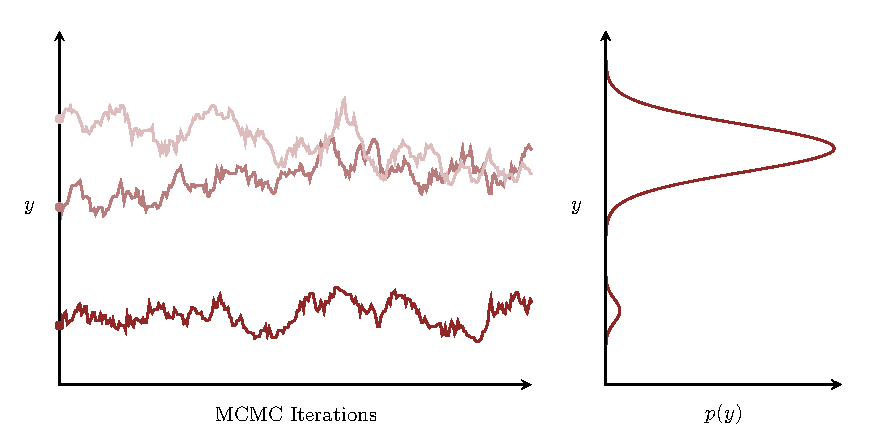
\includegraphics[width=0.9\textwidth,height=\textheight]{figures/multimodal_mcmc/multimodal_mcmc.pdf}

}

\caption{\label{fig-multimodal}Multi-modal posterior distributions are
especially frustrating to Markov chain Monte Carlo. No matter how little
probability is allocated to a mode it can still attract Markov chains
for arbitrarily long times if they are initialized too close to its
basin of attraction.}

\end{figure}%

Redundancy in a mixture model is at its highest when two or more of the
component models are exchangeable, in particular when they span the same
family of probability density functions. In this case we can permute the
corresponding component indices \emph{without affecting any of the model
evaluations}. If \(K_{e}\) component models are exchangeable then the
likelihood function will always exhibit \(K_{e}!\) distinct modes, one
for each permutation of the redundant indices
(Figure~\ref{fig-label-switching}).

\begin{figure}

\begin{minipage}{0.28\linewidth}
~\end{minipage}%
%
\begin{minipage}{0.45\linewidth}

\centering{

\captionsetup{labelsep=none}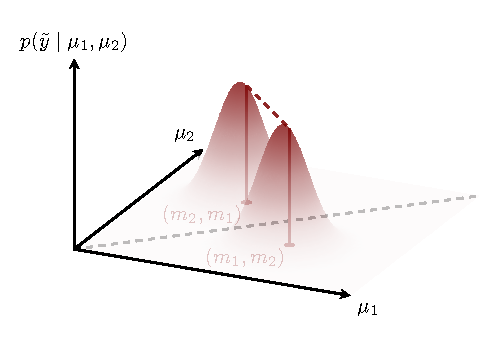
\includegraphics{figures/label_switching/likelihood/likelihood.pdf}

}

\subcaption{\label{fig-label-switching-like}}

\end{minipage}%
%
\begin{minipage}{0.28\linewidth}
~\end{minipage}%
\newline
\begin{minipage}{0.05\linewidth}
~\end{minipage}%
%
\begin{minipage}{0.45\linewidth}

\centering{

\captionsetup{labelsep=none}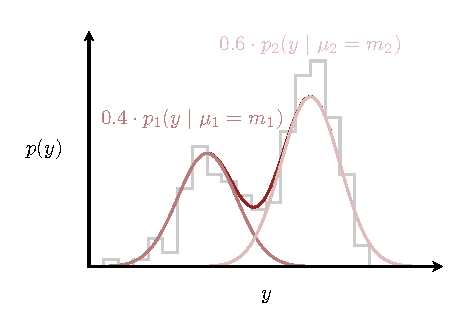
\includegraphics{figures/label_switching/config_one/config_one.pdf}

}

\subcaption{\label{fig-label-switching-1}}

\end{minipage}%
%
\begin{minipage}{0.45\linewidth}

\centering{

\captionsetup{labelsep=none}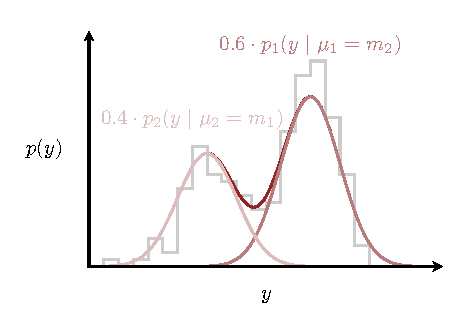
\includegraphics{figures/label_switching/config_two/config_two.pdf}

}

\subcaption{\label{fig-label-switching-2}}

\end{minipage}%
%
\begin{minipage}{0.05\linewidth}
~\end{minipage}%

\caption{\label{fig-label-switching}Exchangeable mixture models with
\(K\) components are formally non-identified -- every model
configuration is accompanied by \(K! - 1\) other model configurations
that define exactly the same data generating process, each found in a
different mode. For example a mixture model with two identical normal
component models always results in (a) a bimodal likelihood function
where (b) every model configuration in one mode is paired with (c) a
model configuration in another mode where the components are swapped.}

\end{figure}%

That said non-exchangeable mixture models are not guaranteed to be
well-behaved either. Degeneracies can also arise when component models
are mathematically distinct but contain similar qualitative behaviors.
Consider, for example, a mixture model over positive integers that
inflates a baseline Poisson model, \(\mathrm{Poisson}(y \mid \lambda)\),
with a Dirac probability distribution concentrating at zero,
\(\delta_{0}(y)\).

If \(\lambda\) is far from zero then these two components exhibit
distinct behaviors, with the former concentrating on values above zero
and the latter on values exactly at zero
(Figure~\ref{fig-zip_degen-separated}). When \(\lambda\) is close to
zero, however, the two component models will both concentrate at zero
(Figure~\ref{fig-zip_degen-overlapping}). In this case observations
\(y = 0\) cannot distinguish between the two components.

\begin{figure}

\begin{minipage}{0.05\linewidth}
~\end{minipage}%
%
\begin{minipage}{0.45\linewidth}

\centering{

\captionsetup{labelsep=none}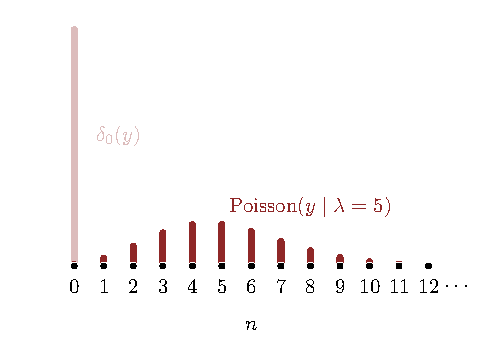
\includegraphics{figures/zip_degen/separated/separated.pdf}

}

\subcaption{\label{fig-zip_degen-separated}}

\end{minipage}%
%
\begin{minipage}{0.45\linewidth}

\centering{

\captionsetup{labelsep=none}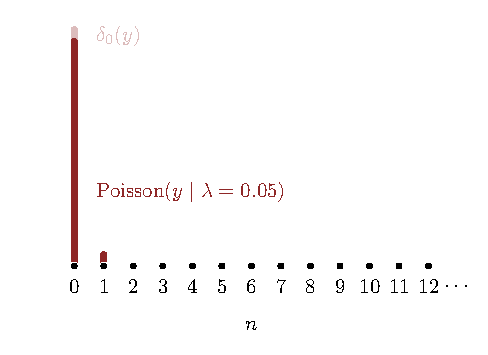
\includegraphics{figures/zip_degen/overlapping/overlapping.pdf}

}

\subcaption{\label{fig-zip_degen-overlapping}}

\end{minipage}%

\caption{\label{fig-zip_degen}Discrete inflation models are prone to
degeneracies when the baseline component can contort itself to mimic the
inflated component. (a) When \(\lambda\) is much larger than zero a
Poisson model is not easily confused with a Dirac model concentrating at
zero. (b) If \(\lambda\) is close to zero, however, then the two
component models are nearly indistinguishable.}

\end{figure}%

In my opinion the most productive approach to mixture modeling is to
treat each component as a model for a distinct data generating process.
Any domain expertise that distinguishes the possible outputs from these
data generating processes can then be directly incorporated into either
the structure of the component models or the prior model to avoid as
much inferential degeneracy as possible.

\section{Demonstrations}\label{demonstrations}

Enough of the generality. In this section we'll demonstrate the basic
mixture modeling techniques presented so in this chapter in specific
exercises.

\subsection{Setup}\label{setup}

Always we start by setting up our local environment.

\begin{Shaded}
\begin{Highlighting}[]
\FunctionTok{par}\NormalTok{(}\AttributeTok{family=}\StringTok{"serif"}\NormalTok{, }\AttributeTok{las=}\DecValTok{1}\NormalTok{, }\AttributeTok{bty=}\StringTok{"l"}\NormalTok{,}
    \AttributeTok{cex.axis=}\DecValTok{1}\NormalTok{, }\AttributeTok{cex.lab=}\DecValTok{1}\NormalTok{, }\AttributeTok{cex.main=}\DecValTok{1}\NormalTok{,}
    \AttributeTok{xaxs=}\StringTok{"i"}\NormalTok{, }\AttributeTok{yaxs=}\StringTok{"i"}\NormalTok{, }\AttributeTok{mar =} \FunctionTok{c}\NormalTok{(}\DecValTok{5}\NormalTok{, }\DecValTok{5}\NormalTok{, }\DecValTok{3}\NormalTok{, }\DecValTok{1}\NormalTok{))}

\FunctionTok{library}\NormalTok{(rstan)}
\FunctionTok{rstan\_options}\NormalTok{(}\AttributeTok{auto\_write =} \ConstantTok{TRUE}\NormalTok{)            }\CommentTok{\# Cache compiled Stan programs}
\FunctionTok{options}\NormalTok{(}\AttributeTok{mc.cores =}\NormalTok{ parallel}\SpecialCharTok{::}\FunctionTok{detectCores}\NormalTok{()) }\CommentTok{\# Parallelize chains}
\NormalTok{parallel}\SpecialCharTok{:::}\FunctionTok{setDefaultClusterOptions}\NormalTok{(}\AttributeTok{setup\_strategy =} \StringTok{"sequential"}\NormalTok{)}
\end{Highlighting}
\end{Shaded}

\begin{Shaded}
\begin{Highlighting}[]
\NormalTok{util }\OtherTok{\textless{}{-}} \FunctionTok{new.env}\NormalTok{()}
\FunctionTok{source}\NormalTok{(}\StringTok{\textquotesingle{}mcmc\_analysis\_tools\_rstan.R\textquotesingle{}}\NormalTok{, }\AttributeTok{local=}\NormalTok{util)}
\FunctionTok{source}\NormalTok{(}\StringTok{\textquotesingle{}mcmc\_visualization\_tools.R\textquotesingle{}}\NormalTok{, }\AttributeTok{local=}\NormalTok{util)}
\end{Highlighting}
\end{Shaded}

\subsection{Separating Signal and
Background}\label{separating-signal-and-background}

For our first exercise let's consider a simplified version of a particle
physics experiment where we observe individual energy depositions in a
detector. These source of these depositions can be either an irreducible
background or a signal of interest. We'll model the background with a
steeply falling exponential probability density function and the signal
with a Cauchy probability density function that can be derived from
certain physical processes.

Unsurprising given the context of this chapter we can model the overlap
of signal and background with a mixture model. The precise configuration
of the signal and background models here is arbitrary, especially
without units. That said the high background probability is emulative of
actual particle physics experiments.

\begin{Shaded}
\begin{Highlighting}[]
\NormalTok{mu\_signal }\OtherTok{\textless{}{-}} \DecValTok{45}
\NormalTok{sigma\_signal }\OtherTok{\textless{}{-}} \DecValTok{5}
\NormalTok{beta\_back }\OtherTok{\textless{}{-}} \DecValTok{20}
\NormalTok{lambda }\OtherTok{\textless{}{-}} \FloatTok{0.95}

\NormalTok{xs }\OtherTok{\textless{}{-}} \FunctionTok{seq}\NormalTok{(}\DecValTok{0}\NormalTok{, }\DecValTok{100}\NormalTok{, }\DecValTok{1}\NormalTok{)}
\NormalTok{ys }\OtherTok{\textless{}{-}}\NormalTok{ lambda }\SpecialCharTok{*} \FunctionTok{dexp}\NormalTok{(xs, }\DecValTok{1} \SpecialCharTok{/}\NormalTok{ beta\_back) }\SpecialCharTok{+}
\NormalTok{      (}\DecValTok{1} \SpecialCharTok{{-}}\NormalTok{ lambda) }\SpecialCharTok{*} \FunctionTok{dcauchy}\NormalTok{(xs, mu\_signal, sigma\_signal)}

\FunctionTok{par}\NormalTok{(}\AttributeTok{mfrow=}\FunctionTok{c}\NormalTok{(}\DecValTok{1}\NormalTok{, }\DecValTok{1}\NormalTok{), }\AttributeTok{mar=}\FunctionTok{c}\NormalTok{(}\DecValTok{5}\NormalTok{, }\DecValTok{5}\NormalTok{, }\DecValTok{3}\NormalTok{, }\DecValTok{1}\NormalTok{))}

\FunctionTok{plot}\NormalTok{(xs, ys, }\AttributeTok{lwd=}\DecValTok{2}\NormalTok{, }\AttributeTok{type=}\StringTok{"l"}\NormalTok{, }\AttributeTok{col=}\NormalTok{util}\SpecialCharTok{$}\NormalTok{c\_dark,}
     \AttributeTok{main=}\StringTok{"Observational Model"}\NormalTok{,}
     \AttributeTok{xlab=}\StringTok{"y"}\NormalTok{, }\AttributeTok{ylab=}\StringTok{"Probability Density"}\NormalTok{)}
\end{Highlighting}
\end{Shaded}

\includegraphics{mixture_modeling_files/figure-pdf/unnamed-chunk-3-1.pdf}

Simulating data from this model is straightforward using the techniques
introduced in \hyperref[sec:sampling]{Section 1.4}.

\begin{codelisting}

\caption{\texttt{simu\textbackslash\_signal\textbackslash\_background.stan}}

\begin{Shaded}
\begin{Highlighting}[]
\KeywordTok{data}\NormalTok{ \{}
  \DataTypeTok{int}\NormalTok{\textless{}}\KeywordTok{lower}\NormalTok{=}\DecValTok{1}\NormalTok{\textgreater{} N;      }\CommentTok{// Number of observations}
\NormalTok{\}}

\KeywordTok{transformed data}\NormalTok{ \{}
  \DataTypeTok{real}\NormalTok{ mu\_signal =  }\DecValTok{45}\NormalTok{;                 }\CommentTok{// Signal location}
  \DataTypeTok{real}\NormalTok{\textless{}}\KeywordTok{lower}\NormalTok{=}\DecValTok{0}\NormalTok{\textgreater{} sigma\_signal = }\DecValTok{5}\NormalTok{;       }\CommentTok{// Signal scale}
  \DataTypeTok{real}\NormalTok{ beta\_back = }\DecValTok{20}\NormalTok{;                  }\CommentTok{// Background rate}
  \DataTypeTok{real}\NormalTok{\textless{}}\KeywordTok{lower}\NormalTok{=}\DecValTok{0}\NormalTok{, }\KeywordTok{upper}\NormalTok{=}\DecValTok{1}\NormalTok{\textgreater{} lambda = }\FloatTok{0.95}\NormalTok{; }\CommentTok{// Background probability}
\NormalTok{\}}

\KeywordTok{generated quantities}\NormalTok{ \{}
  \DataTypeTok{array}\NormalTok{[N] }\DataTypeTok{real}\NormalTok{\textless{}}\KeywordTok{lower}\NormalTok{=}\DecValTok{0}\NormalTok{\textgreater{} y = rep\_array({-}}\DecValTok{1}\NormalTok{, N);}

  \ControlFlowTok{for}\NormalTok{ (n }\ControlFlowTok{in} \DecValTok{1}\NormalTok{:N) \{}
    \ControlFlowTok{if}\NormalTok{ (bernoulli\_rng(lambda)) \{}
\NormalTok{      y[n] = exponential\_rng(}\DecValTok{1}\NormalTok{ / beta\_back);}
\NormalTok{    \} }\ControlFlowTok{else}\NormalTok{ \{}
      \CommentTok{// Truncate signal to positive values}
      \ControlFlowTok{while}\NormalTok{ (y[n] \textless{} }\DecValTok{0}\NormalTok{) \{}
\NormalTok{        y[n] = cauchy\_rng(mu\_signal, sigma\_signal);}
\NormalTok{      \}}
\NormalTok{    \}}
\NormalTok{  \}}
\NormalTok{\}}
\end{Highlighting}
\end{Shaded}

\end{codelisting}

\begin{Shaded}
\begin{Highlighting}[]
\NormalTok{N }\OtherTok{\textless{}{-}} \DecValTok{500}

\NormalTok{simu }\OtherTok{\textless{}{-}} \FunctionTok{stan}\NormalTok{(}\AttributeTok{file=}\StringTok{"stan\_programs/simu\_signal\_background.stan"}\NormalTok{,}
             \AttributeTok{algorithm=}\StringTok{"Fixed\_param"}\NormalTok{,}
             \AttributeTok{data=}\FunctionTok{list}\NormalTok{(}\StringTok{"N"} \OtherTok{=}\NormalTok{ N), }\AttributeTok{seed=}\DecValTok{8438338}\NormalTok{,}
             \AttributeTok{warmup=}\DecValTok{0}\NormalTok{, }\AttributeTok{iter=}\DecValTok{1}\NormalTok{, }\AttributeTok{chains=}\DecValTok{1}\NormalTok{, }\AttributeTok{refresh=}\DecValTok{0}\NormalTok{)}

\NormalTok{data }\OtherTok{\textless{}{-}} \FunctionTok{list}\NormalTok{(}\StringTok{"N"} \OtherTok{=}\NormalTok{ N,}
             \StringTok{"y"} \OtherTok{=} \FunctionTok{extract}\NormalTok{(simu)}\SpecialCharTok{$}\NormalTok{y[}\DecValTok{1}\NormalTok{,])}
\end{Highlighting}
\end{Shaded}

Because of the overwhelming background contribution it's hard to make
out the meager signal.

\begin{Shaded}
\begin{Highlighting}[]
\FunctionTok{par}\NormalTok{(}\AttributeTok{mfrow=}\FunctionTok{c}\NormalTok{(}\DecValTok{1}\NormalTok{, }\DecValTok{1}\NormalTok{), }\AttributeTok{mar=}\FunctionTok{c}\NormalTok{(}\DecValTok{5}\NormalTok{, }\DecValTok{5}\NormalTok{, }\DecValTok{1}\NormalTok{, }\DecValTok{1}\NormalTok{))}

\NormalTok{util}\SpecialCharTok{$}\FunctionTok{plot\_line\_hist}\NormalTok{(data}\SpecialCharTok{$}\NormalTok{y, }\DecValTok{0}\NormalTok{, }\DecValTok{125}\NormalTok{, }\DecValTok{5}\NormalTok{, }\AttributeTok{xlab=}\StringTok{"y"}\NormalTok{, }\AttributeTok{prob=}\ConstantTok{TRUE}\NormalTok{)}
\end{Highlighting}
\end{Shaded}

\begin{verbatim}
Warning in check_bin_containment(bin_min, bin_max, values): 1 value (0.2%) fell
above the binning.
\end{verbatim}

\includegraphics{mixture_modeling_files/figure-pdf/unnamed-chunk-5-1.pdf}

Perhaps we can use Bayesian inference to tease out the signal?

Note that the prior model here is somewhat arbitrary due to the nature
of the exercise. In a practical analysis we would want to take care to
elicit at least some basic domain expertise about the behaviors captured
by each parameter. This is especially true if the component models have
any potential for redundant behaviors.

\begin{codelisting}

\caption{\texttt{signal\textbackslash\_background1.stan}}

\begin{Shaded}
\begin{Highlighting}[]
\KeywordTok{data}\NormalTok{ \{}
  \CommentTok{// Signal and background observations}
  \DataTypeTok{int}\NormalTok{\textless{}}\KeywordTok{lower}\NormalTok{=}\DecValTok{1}\NormalTok{\textgreater{} N;}
  \DataTypeTok{array}\NormalTok{[N] }\DataTypeTok{real}\NormalTok{\textless{}}\KeywordTok{lower}\NormalTok{=}\DecValTok{0}\NormalTok{\textgreater{} y;}
\NormalTok{\}}

\KeywordTok{parameters}\NormalTok{ \{}
  \DataTypeTok{real}\NormalTok{ mu\_signal;                }\CommentTok{// Signal location}
  \DataTypeTok{real}\NormalTok{\textless{}}\KeywordTok{lower}\NormalTok{=}\DecValTok{0}\NormalTok{\textgreater{} sigma\_signal;    }\CommentTok{// Signal scale}
  \DataTypeTok{real}\NormalTok{\textless{}}\KeywordTok{lower}\NormalTok{=}\DecValTok{0}\NormalTok{\textgreater{} beta\_back;       }\CommentTok{// Background scale}
  \DataTypeTok{real}\NormalTok{\textless{}}\KeywordTok{lower}\NormalTok{=}\DecValTok{0}\NormalTok{, }\KeywordTok{upper}\NormalTok{=}\DecValTok{1}\NormalTok{\textgreater{} lambda; }\CommentTok{// Background probability}
\NormalTok{\}}

\KeywordTok{model}\NormalTok{ \{}
  \CommentTok{// Prior model}
\NormalTok{  mu\_signal \textasciitilde{} normal(}\DecValTok{50}\NormalTok{, }\DecValTok{50}\NormalTok{ / }\FloatTok{2.32}\NormalTok{);   }\CommentTok{// 0 \textless{}\textasciitilde{} mu\_signal    \textless{}\textasciitilde{} 100}
\NormalTok{  sigma\_signal \textasciitilde{} normal(}\DecValTok{0}\NormalTok{, }\DecValTok{25}\NormalTok{ / }\FloatTok{2.57}\NormalTok{); }\CommentTok{// 0 \textless{}\textasciitilde{} sigma\_signal \textless{}\textasciitilde{}  25}
\NormalTok{  beta\_back \textasciitilde{} normal(}\DecValTok{0}\NormalTok{, }\DecValTok{50}\NormalTok{ / }\FloatTok{2.57}\NormalTok{);    }\CommentTok{// 0 \textless{}\textasciitilde{} beta\_back    \textless{}\textasciitilde{}  50}
  \CommentTok{// Implicit uniform prior density function for lambda}

  \CommentTok{// Observational model}
  \ControlFlowTok{for}\NormalTok{ (n }\ControlFlowTok{in} \DecValTok{1}\NormalTok{:N) \{}
    \KeywordTok{target +=}\NormalTok{ log\_mix(lambda,}
\NormalTok{                      exponential\_lpdf(y[n] | }\DecValTok{1}\NormalTok{ / beta\_back),}
\NormalTok{                      cauchy\_lpdf(y[n] | mu\_signal, sigma\_signal));}
\NormalTok{  \}}
\NormalTok{\}}

\KeywordTok{generated quantities}\NormalTok{ \{}
  \DataTypeTok{array}\NormalTok{[N] }\DataTypeTok{real}\NormalTok{\textless{}}\KeywordTok{lower}\NormalTok{=}\DecValTok{0}\NormalTok{\textgreater{} y\_pred = rep\_array({-}}\DecValTok{1}\NormalTok{, N);}

  \ControlFlowTok{for}\NormalTok{ (n }\ControlFlowTok{in} \DecValTok{1}\NormalTok{:N) \{}
    \ControlFlowTok{if}\NormalTok{ (bernoulli\_rng(lambda)) \{}
\NormalTok{      y\_pred[n] = exponential\_rng(}\DecValTok{1}\NormalTok{ / beta\_back);}
\NormalTok{    \} }\ControlFlowTok{else}\NormalTok{ \{}
      \ControlFlowTok{while}\NormalTok{ (y\_pred[n] \textless{} }\DecValTok{0}\NormalTok{) \{}
\NormalTok{        y\_pred[n] = cauchy\_rng(mu\_signal, sigma\_signal);}
\NormalTok{      \}}
\NormalTok{    \}}
\NormalTok{  \}}
\NormalTok{\}}
\end{Highlighting}
\end{Shaded}

\end{codelisting}

\begin{Shaded}
\begin{Highlighting}[]
\NormalTok{fit }\OtherTok{\textless{}{-}} \FunctionTok{stan}\NormalTok{(}\AttributeTok{file=}\StringTok{"stan\_programs/signal\_background1.stan"}\NormalTok{,}
            \AttributeTok{data=}\NormalTok{data, }\AttributeTok{seed=}\DecValTok{8438338}\NormalTok{,}
            \AttributeTok{warmup=}\DecValTok{1000}\NormalTok{, }\AttributeTok{iter=}\DecValTok{2024}\NormalTok{, }\AttributeTok{refresh=}\DecValTok{0}\NormalTok{)}
\end{Highlighting}
\end{Shaded}

The diagnostics exhibit some mild \(\hat{\xi}\) warnings, but nothing
too concerning so long as we're not interested in the expectation value
of \texttt{mu\_signal}.

\begin{Shaded}
\begin{Highlighting}[]
\NormalTok{diagnostics }\OtherTok{\textless{}{-}}\NormalTok{ util}\SpecialCharTok{$}\FunctionTok{extract\_hmc\_diagnostics}\NormalTok{(fit)}
\NormalTok{util}\SpecialCharTok{$}\FunctionTok{check\_all\_hmc\_diagnostics}\NormalTok{(diagnostics)}
\end{Highlighting}
\end{Shaded}

\begin{verbatim}
  All Hamiltonian Monte Carlo diagnostics are consistent with reliable
Markov chain Monte Carlo.
\end{verbatim}

\begin{Shaded}
\begin{Highlighting}[]
\NormalTok{samples }\OtherTok{\textless{}{-}}\NormalTok{ util}\SpecialCharTok{$}\FunctionTok{extract\_expectand\_vals}\NormalTok{(fit)}
\NormalTok{base\_samples }\OtherTok{\textless{}{-}}\NormalTok{ util}\SpecialCharTok{$}\FunctionTok{filter\_expectands}\NormalTok{(samples,}
                                       \FunctionTok{c}\NormalTok{(}\StringTok{\textquotesingle{}mu\_signal\textquotesingle{}}\NormalTok{, }\StringTok{\textquotesingle{}sigma\_signal\textquotesingle{}}\NormalTok{,}
                                         \StringTok{\textquotesingle{}beta\_back\textquotesingle{}}\NormalTok{, }\StringTok{\textquotesingle{}lambda\textquotesingle{}}\NormalTok{))}
\NormalTok{util}\SpecialCharTok{$}\FunctionTok{check\_all\_expectand\_diagnostics}\NormalTok{(base\_samples)}
\end{Highlighting}
\end{Shaded}

\begin{verbatim}
mu_signal:
  Chain 1: Right tail hat{xi} (0.253) exceeds 0.25.
  Chain 3: Right tail hat{xi} (0.423) exceeds 0.25.
  Chain 4: Right tail hat{xi} (0.378) exceeds 0.25.


Large tail hat{xi}s suggest that the expectand might not be
sufficiently integrable.
\end{verbatim}

Even better there are no indications of retrodictive tension that would
suggest inadequacies in our model.

\begin{Shaded}
\begin{Highlighting}[]
\FunctionTok{par}\NormalTok{(}\AttributeTok{mfrow=}\FunctionTok{c}\NormalTok{(}\DecValTok{1}\NormalTok{, }\DecValTok{1}\NormalTok{), }\AttributeTok{mar=}\FunctionTok{c}\NormalTok{(}\DecValTok{5}\NormalTok{, }\DecValTok{5}\NormalTok{, }\DecValTok{1}\NormalTok{, }\DecValTok{1}\NormalTok{))}

\NormalTok{util}\SpecialCharTok{$}\FunctionTok{plot\_hist\_quantiles}\NormalTok{(samples, }\StringTok{\textquotesingle{}y\_pred\textquotesingle{}}\NormalTok{, }\DecValTok{0}\NormalTok{, }\DecValTok{125}\NormalTok{, }\DecValTok{5}\NormalTok{,}
                         \AttributeTok{baseline\_values=}\NormalTok{data}\SpecialCharTok{$}\NormalTok{y, }\AttributeTok{xlab=}\StringTok{"y"}\NormalTok{)}
\end{Highlighting}
\end{Shaded}

\begin{verbatim}
Warning in check_bin_containment(bin_min, bin_max, collapsed_values,
"predictive value"): 6981 predictive values (0.3%) fell above the binning.
\end{verbatim}

\begin{verbatim}
Warning in check_bin_containment(bin_min, bin_max, baseline_values, "observed
value"): 1 observed value (0.2%) fell above the binning.
\end{verbatim}

\includegraphics{mixture_modeling_files/figure-pdf/unnamed-chunk-8-1.pdf}

Our posterior inferences are not too bad, especially considering the
relatively small number of observations and overwhelming background
contribution. Note also the heavy tails of marginal posterior
distribution for \texttt{mu\_signal}, consistent with the \(\hat{\xi}\)
warnings.

\begin{Shaded}
\begin{Highlighting}[]
\FunctionTok{par}\NormalTok{(}\AttributeTok{mfrow=}\FunctionTok{c}\NormalTok{(}\DecValTok{2}\NormalTok{, }\DecValTok{2}\NormalTok{), }\AttributeTok{mar=}\FunctionTok{c}\NormalTok{(}\DecValTok{5}\NormalTok{, }\DecValTok{5}\NormalTok{, }\DecValTok{1}\NormalTok{, }\DecValTok{1}\NormalTok{))}

\NormalTok{util}\SpecialCharTok{$}\FunctionTok{plot\_expectand\_pushforward}\NormalTok{(samples[[}\StringTok{\textquotesingle{}mu\_signal\textquotesingle{}}\NormalTok{]], }\DecValTok{25}\NormalTok{,}
                                \AttributeTok{display\_name=}\StringTok{"mu\_signal"}\NormalTok{,}
                                \AttributeTok{baseline=}\NormalTok{mu\_signal,}
                                \AttributeTok{baseline\_col=}\NormalTok{util}\SpecialCharTok{$}\NormalTok{c\_mid\_teal)}

\NormalTok{util}\SpecialCharTok{$}\FunctionTok{plot\_expectand\_pushforward}\NormalTok{(samples[[}\StringTok{\textquotesingle{}sigma\_signal\textquotesingle{}}\NormalTok{]], }\DecValTok{25}\NormalTok{,}
                                \AttributeTok{display\_name=}\StringTok{"sigma\_signal"}\NormalTok{,}
                                \AttributeTok{baseline=}\NormalTok{sigma\_signal,}
                                \AttributeTok{baseline\_col=}\NormalTok{util}\SpecialCharTok{$}\NormalTok{c\_mid\_teal)}

\NormalTok{util}\SpecialCharTok{$}\FunctionTok{plot\_expectand\_pushforward}\NormalTok{(samples[[}\StringTok{\textquotesingle{}beta\_back\textquotesingle{}}\NormalTok{]], }\DecValTok{25}\NormalTok{,}
                                \AttributeTok{display\_name=}\StringTok{"beta\_back"}\NormalTok{,}
                                \AttributeTok{baseline=}\NormalTok{beta\_back,}
                                \AttributeTok{baseline\_col=}\NormalTok{util}\SpecialCharTok{$}\NormalTok{c\_mid\_teal)}

\NormalTok{util}\SpecialCharTok{$}\FunctionTok{plot\_expectand\_pushforward}\NormalTok{(samples[[}\StringTok{\textquotesingle{}lambda\textquotesingle{}}\NormalTok{]], }\DecValTok{25}\NormalTok{,}
                                \AttributeTok{display\_name=}\StringTok{"lambda"}\NormalTok{,}
                                \AttributeTok{baseline=}\NormalTok{lambda,}
                                \AttributeTok{baseline\_col=}\NormalTok{util}\SpecialCharTok{$}\NormalTok{c\_mid\_teal)}
\end{Highlighting}
\end{Shaded}

\includegraphics{mixture_modeling_files/figure-pdf/unnamed-chunk-9-1.pdf}

We can also directly visualize the inferred behaviors of the signal
model, the background model, and their combinations.

\begin{Shaded}
\begin{Highlighting}[]
\FunctionTok{library}\NormalTok{(colormap)}
\NormalTok{nom\_colors }\OtherTok{\textless{}{-}} \FunctionTok{c}\NormalTok{(}\StringTok{"\#DCBCBC"}\NormalTok{, }\StringTok{"\#C79999"}\NormalTok{, }\StringTok{"\#B97C7C"}\NormalTok{,}
                \StringTok{"\#A25050"}\NormalTok{, }\StringTok{"\#8F2727"}\NormalTok{, }\StringTok{"\#7C0000"}\NormalTok{)}
\NormalTok{line\_colors }\OtherTok{\textless{}{-}} \FunctionTok{colormap}\NormalTok{(}\AttributeTok{colormap=}\NormalTok{nom\_colors, }\AttributeTok{nshades=}\DecValTok{20}\NormalTok{)}

\NormalTok{cs }\OtherTok{\textless{}{-}} \FunctionTok{c}\NormalTok{(}\DecValTok{1}\NormalTok{, }\DecValTok{2}\NormalTok{, }\DecValTok{3}\NormalTok{, }\DecValTok{4}\NormalTok{)}
\NormalTok{ss }\OtherTok{\textless{}{-}} \FunctionTok{c}\NormalTok{(}\DecValTok{1}\NormalTok{, }\DecValTok{250}\NormalTok{, }\DecValTok{500}\NormalTok{, }\DecValTok{750}\NormalTok{, }\DecValTok{1000}\NormalTok{)}

\NormalTok{plot\_signal\_realizations }\OtherTok{\textless{}{-}} \ControlFlowTok{function}\NormalTok{() \{}
\NormalTok{  n }\OtherTok{\textless{}{-}} \DecValTok{1}
  \ControlFlowTok{for}\NormalTok{ (c }\ControlFlowTok{in}\NormalTok{ cs) \{}
    \ControlFlowTok{for}\NormalTok{ (s }\ControlFlowTok{in}\NormalTok{ ss) \{}
\NormalTok{      ms }\OtherTok{\textless{}{-}}\NormalTok{ samples[[}\StringTok{\textquotesingle{}mu\_signal\textquotesingle{}}\NormalTok{]][c, s]}
\NormalTok{      ss }\OtherTok{\textless{}{-}}\NormalTok{ samples[[}\StringTok{\textquotesingle{}sigma\_signal\textquotesingle{}}\NormalTok{]][c, s]}
\NormalTok{      l }\OtherTok{\textless{}{-}}\NormalTok{ samples[[}\StringTok{\textquotesingle{}lambda\textquotesingle{}}\NormalTok{]][c, s]}

\NormalTok{      ys }\OtherTok{\textless{}{-}}\NormalTok{ (}\DecValTok{1} \SpecialCharTok{{-}}\NormalTok{ l) }\SpecialCharTok{*} \FunctionTok{dcauchy}\NormalTok{(xs, ms, ss)}
      \FunctionTok{lines}\NormalTok{(xs, ys, }\AttributeTok{lwd=}\DecValTok{2}\NormalTok{, }\AttributeTok{col=}\NormalTok{line\_colors[n])}
\NormalTok{      n }\OtherTok{\textless{}{-}}\NormalTok{ n }\SpecialCharTok{+} \DecValTok{1}
\NormalTok{    \}}
\NormalTok{  \}}
\NormalTok{  ys }\OtherTok{\textless{}{-}}\NormalTok{ (}\DecValTok{1} \SpecialCharTok{{-}}\NormalTok{ lambda) }\SpecialCharTok{*} \FunctionTok{dcauchy}\NormalTok{(xs, mu\_signal, sigma\_signal)}
  \FunctionTok{lines}\NormalTok{(xs, ys, }\AttributeTok{lwd=}\DecValTok{4}\NormalTok{, }\AttributeTok{col=}\StringTok{"white"}\NormalTok{)}
  \FunctionTok{lines}\NormalTok{(xs, ys, }\AttributeTok{lwd=}\DecValTok{2}\NormalTok{, }\AttributeTok{col=}\NormalTok{util}\SpecialCharTok{$}\NormalTok{c\_dark\_teal)}
\NormalTok{\}}

\NormalTok{plot\_back\_realizations }\OtherTok{\textless{}{-}} \ControlFlowTok{function}\NormalTok{() \{}
\NormalTok{  n }\OtherTok{\textless{}{-}} \DecValTok{1}
  \ControlFlowTok{for}\NormalTok{ (c }\ControlFlowTok{in}\NormalTok{ cs) \{}
    \ControlFlowTok{for}\NormalTok{ (s }\ControlFlowTok{in}\NormalTok{ ss) \{}
\NormalTok{      bb }\OtherTok{\textless{}{-}}\NormalTok{ samples[[}\StringTok{\textquotesingle{}beta\_back\textquotesingle{}}\NormalTok{]][c, s]}
\NormalTok{      l }\OtherTok{\textless{}{-}}\NormalTok{ samples[[}\StringTok{\textquotesingle{}lambda\textquotesingle{}}\NormalTok{]][c, s]}

\NormalTok{      ys }\OtherTok{\textless{}{-}}\NormalTok{ l }\SpecialCharTok{*} \FunctionTok{dexp}\NormalTok{(xs, }\DecValTok{1} \SpecialCharTok{/}\NormalTok{ bb)}
      \FunctionTok{lines}\NormalTok{(xs, ys, }\AttributeTok{lwd=}\DecValTok{2}\NormalTok{, }\AttributeTok{col=}\NormalTok{line\_colors[n])}
\NormalTok{      n }\OtherTok{\textless{}{-}}\NormalTok{ n }\SpecialCharTok{+} \DecValTok{1}
\NormalTok{    \}}
\NormalTok{  \}}
\NormalTok{  ys }\OtherTok{\textless{}{-}}\NormalTok{ lambda }\SpecialCharTok{*} \FunctionTok{dexp}\NormalTok{(xs, }\DecValTok{1} \SpecialCharTok{/}\NormalTok{ beta\_back)}
  \FunctionTok{lines}\NormalTok{(xs, ys, }\AttributeTok{lwd=}\DecValTok{4}\NormalTok{, }\AttributeTok{col=}\StringTok{"white"}\NormalTok{)}
  \FunctionTok{lines}\NormalTok{(xs, ys, }\AttributeTok{lwd=}\DecValTok{2}\NormalTok{, }\AttributeTok{col=}\NormalTok{util}\SpecialCharTok{$}\NormalTok{c\_dark\_teal)}
\NormalTok{\}}

\NormalTok{plot\_sum\_realizations }\OtherTok{\textless{}{-}} \ControlFlowTok{function}\NormalTok{() \{}
\NormalTok{  n }\OtherTok{\textless{}{-}} \DecValTok{1}
  \ControlFlowTok{for}\NormalTok{ (c }\ControlFlowTok{in}\NormalTok{ cs) \{}
    \ControlFlowTok{for}\NormalTok{ (s }\ControlFlowTok{in}\NormalTok{ ss) \{}
\NormalTok{      ms }\OtherTok{\textless{}{-}}\NormalTok{ samples[[}\StringTok{\textquotesingle{}mu\_signal\textquotesingle{}}\NormalTok{]][c, s]}
\NormalTok{      ss }\OtherTok{\textless{}{-}}\NormalTok{ samples[[}\StringTok{\textquotesingle{}sigma\_signal\textquotesingle{}}\NormalTok{]][c, s]}
\NormalTok{      bb }\OtherTok{\textless{}{-}}\NormalTok{ samples[[}\StringTok{\textquotesingle{}beta\_back\textquotesingle{}}\NormalTok{]][c, s]}
\NormalTok{      l }\OtherTok{\textless{}{-}}\NormalTok{ samples[[}\StringTok{\textquotesingle{}lambda\textquotesingle{}}\NormalTok{]][c, s]}

\NormalTok{      ys }\OtherTok{\textless{}{-}}\NormalTok{ l }\SpecialCharTok{*} \FunctionTok{dexp}\NormalTok{(xs, }\DecValTok{1} \SpecialCharTok{/}\NormalTok{ bb) }\SpecialCharTok{+}\NormalTok{ (}\DecValTok{1} \SpecialCharTok{{-}}\NormalTok{ l) }\SpecialCharTok{*} \FunctionTok{dcauchy}\NormalTok{(xs, ms, ss)}
      \FunctionTok{lines}\NormalTok{(xs, ys, }\AttributeTok{lwd=}\DecValTok{2}\NormalTok{, }\AttributeTok{col=}\NormalTok{line\_colors[n])}
\NormalTok{      n }\OtherTok{\textless{}{-}}\NormalTok{ n }\SpecialCharTok{+} \DecValTok{1}
\NormalTok{    \}}
\NormalTok{  \}}
\NormalTok{  ys }\OtherTok{\textless{}{-}}\NormalTok{ (}\DecValTok{1} \SpecialCharTok{{-}}\NormalTok{ lambda) }\SpecialCharTok{*} \FunctionTok{dcauchy}\NormalTok{(xs, mu\_signal, sigma\_signal) }\SpecialCharTok{+}
\NormalTok{        lambda }\SpecialCharTok{*} \FunctionTok{dexp}\NormalTok{(xs, }\DecValTok{1} \SpecialCharTok{/}\NormalTok{ beta\_back)}
  \FunctionTok{lines}\NormalTok{(xs, ys, }\AttributeTok{lwd=}\DecValTok{4}\NormalTok{, }\AttributeTok{col=}\StringTok{"white"}\NormalTok{)}
  \FunctionTok{lines}\NormalTok{(xs, ys, }\AttributeTok{lwd=}\DecValTok{2}\NormalTok{, }\AttributeTok{col=}\NormalTok{util}\SpecialCharTok{$}\NormalTok{c\_dark\_teal)}
\NormalTok{\}}
\end{Highlighting}
\end{Shaded}

While the posterior uncertainties are large we do seem to be able to
resolve the underlying signal through the overwhelming background!

\begin{Shaded}
\begin{Highlighting}[]
\FunctionTok{par}\NormalTok{(}\AttributeTok{mfrow=}\FunctionTok{c}\NormalTok{(}\DecValTok{1}\NormalTok{, }\DecValTok{3}\NormalTok{), }\AttributeTok{mar=}\FunctionTok{c}\NormalTok{(}\DecValTok{5}\NormalTok{, }\DecValTok{5}\NormalTok{, }\DecValTok{2}\NormalTok{, }\DecValTok{1}\NormalTok{))}

\NormalTok{xs }\OtherTok{\textless{}{-}} \FunctionTok{seq}\NormalTok{(}\DecValTok{0}\NormalTok{, }\DecValTok{100}\NormalTok{, }\FloatTok{0.5}\NormalTok{)}

\FunctionTok{plot}\NormalTok{(}\ConstantTok{NULL}\NormalTok{, }\AttributeTok{main=}\StringTok{"Weighted Signal"}\NormalTok{,}
     \AttributeTok{xlab=}\StringTok{"y"}\NormalTok{, }\AttributeTok{ylab=}\StringTok{"Probability Density"}\NormalTok{,}
     \AttributeTok{xlim=}\FunctionTok{range}\NormalTok{(xs), }\AttributeTok{ylim=}\FunctionTok{c}\NormalTok{(}\DecValTok{0}\NormalTok{, }\FloatTok{0.05}\NormalTok{))}
\FunctionTok{plot\_signal\_realizations}\NormalTok{()}

\FunctionTok{plot}\NormalTok{(}\ConstantTok{NULL}\NormalTok{, }\AttributeTok{main=}\StringTok{"Weighted Background"}\NormalTok{,}
     \AttributeTok{xlab=}\StringTok{"y"}\NormalTok{, }\AttributeTok{ylab=}\StringTok{"Probability Density"}\NormalTok{,}
     \AttributeTok{xlim=}\FunctionTok{range}\NormalTok{(xs), }\AttributeTok{ylim=}\FunctionTok{c}\NormalTok{(}\DecValTok{0}\NormalTok{, }\FloatTok{0.05}\NormalTok{))}
\FunctionTok{plot\_back\_realizations}\NormalTok{()}

\FunctionTok{plot}\NormalTok{(}\ConstantTok{NULL}\NormalTok{, }\AttributeTok{main=}\StringTok{"Mixture"}\NormalTok{,}
     \AttributeTok{xlab=}\StringTok{"y"}\NormalTok{, }\AttributeTok{ylab=}\StringTok{"Probability Density"}\NormalTok{,}
     \AttributeTok{xlim=}\FunctionTok{range}\NormalTok{(xs), }\AttributeTok{ylim=}\FunctionTok{c}\NormalTok{(}\DecValTok{0}\NormalTok{, }\FloatTok{0.05}\NormalTok{))}
\FunctionTok{plot\_sum\_realizations}\NormalTok{()}
\end{Highlighting}
\end{Shaded}

\includegraphics{mixture_modeling_files/figure-pdf/unnamed-chunk-11-1.pdf}

In many scientific applications the relative proportion of signal and
background, and hence the component probabilities, are more relevant
than the probability that any particular observation arose from either
source. That said if the latter is of interest then we computing
posterior assignment probabilities and simulating assignments is
straightforward.

\begin{codelisting}

\caption{\texttt{signal\textbackslash\_background2.stan}}

\begin{Shaded}
\begin{Highlighting}[]
\KeywordTok{data}\NormalTok{ \{}
  \CommentTok{// Signal and background observations}
  \DataTypeTok{int}\NormalTok{\textless{}}\KeywordTok{lower}\NormalTok{=}\DecValTok{1}\NormalTok{\textgreater{} N;}
  \DataTypeTok{array}\NormalTok{[N] }\DataTypeTok{real}\NormalTok{\textless{}}\KeywordTok{lower}\NormalTok{=}\DecValTok{0}\NormalTok{\textgreater{} y;}
\NormalTok{\}}

\KeywordTok{parameters}\NormalTok{ \{}
  \DataTypeTok{real}\NormalTok{ mu\_signal;                }\CommentTok{// Signal location}
  \DataTypeTok{real}\NormalTok{\textless{}}\KeywordTok{lower}\NormalTok{=}\DecValTok{0}\NormalTok{\textgreater{} sigma\_signal;    }\CommentTok{// Signal scale}
  \DataTypeTok{real}\NormalTok{\textless{}}\KeywordTok{lower}\NormalTok{=}\DecValTok{0}\NormalTok{\textgreater{} beta\_back;       }\CommentTok{// Background scale}
  \DataTypeTok{real}\NormalTok{\textless{}}\KeywordTok{lower}\NormalTok{=}\DecValTok{0}\NormalTok{, }\KeywordTok{upper}\NormalTok{=}\DecValTok{1}\NormalTok{\textgreater{} lambda; }\CommentTok{// Background probability}
\NormalTok{\}}

\KeywordTok{model}\NormalTok{ \{}
  \CommentTok{// Prior model}
\NormalTok{  mu\_signal \textasciitilde{} normal(}\DecValTok{50}\NormalTok{, }\DecValTok{50}\NormalTok{ / }\FloatTok{2.32}\NormalTok{);   }\CommentTok{// 0 \textless{}\textasciitilde{} mu\_signal    \textless{}\textasciitilde{} 100}
\NormalTok{  sigma\_signal \textasciitilde{} normal(}\DecValTok{0}\NormalTok{, }\DecValTok{25}\NormalTok{ / }\FloatTok{2.57}\NormalTok{); }\CommentTok{// 0 \textless{}\textasciitilde{} sigma\_signal \textless{}\textasciitilde{}  25}
\NormalTok{  beta\_back \textasciitilde{} normal(}\DecValTok{0}\NormalTok{, }\DecValTok{50}\NormalTok{ / }\FloatTok{2.57}\NormalTok{);    }\CommentTok{// 0 \textless{}\textasciitilde{} beta\_back    \textless{}\textasciitilde{}  50}
  \CommentTok{// Implicit uniform prior density function for lambda}

  \CommentTok{// Observational model}
  \ControlFlowTok{for}\NormalTok{ (n }\ControlFlowTok{in} \DecValTok{1}\NormalTok{:N) \{}
    \KeywordTok{target +=}\NormalTok{ log\_mix(lambda,}
\NormalTok{                      exponential\_lpdf(y[n] | }\DecValTok{1}\NormalTok{ / beta\_back),}
\NormalTok{                      cauchy\_lpdf(y[n] | mu\_signal, sigma\_signal));}
\NormalTok{  \}}
\NormalTok{\}}

\KeywordTok{generated quantities}\NormalTok{ \{}
  \DataTypeTok{array}\NormalTok{[N] }\DataTypeTok{real}\NormalTok{\textless{}}\KeywordTok{lower}\NormalTok{=}\DecValTok{0}\NormalTok{, }\KeywordTok{upper}\NormalTok{=}\DecValTok{1}\NormalTok{\textgreater{} p;}
  \DataTypeTok{array}\NormalTok{[N] }\DataTypeTok{int}\NormalTok{\textless{}}\KeywordTok{lower}\NormalTok{=}\DecValTok{0}\NormalTok{, }\KeywordTok{upper}\NormalTok{=}\DecValTok{1}\NormalTok{\textgreater{} z\_pred;}

  \ControlFlowTok{for}\NormalTok{ (n }\ControlFlowTok{in} \DecValTok{1}\NormalTok{:N) \{}
    \DataTypeTok{vector}\NormalTok{[}\DecValTok{2}\NormalTok{] xs = [   log(lambda)}
\NormalTok{                     + exponential\_lpdf(y[n] | }\DecValTok{1}\NormalTok{ / beta\_back),}
\NormalTok{                       log(}\DecValTok{1}\NormalTok{ {-} lambda)}
\NormalTok{                     + cauchy\_lpdf(y[n] | mu\_signal, sigma\_signal) ]\textquotesingle{};}
\NormalTok{    p[n] = softmax(xs)[}\DecValTok{1}\NormalTok{];}
\NormalTok{    z\_pred[n] = bernoulli\_rng(p[n]);}
\NormalTok{  \}}
\NormalTok{\}}
\end{Highlighting}
\end{Shaded}

\end{codelisting}

\begin{Shaded}
\begin{Highlighting}[]
\NormalTok{fit }\OtherTok{\textless{}{-}} \FunctionTok{stan}\NormalTok{(}\AttributeTok{file=}\StringTok{"stan\_programs/signal\_background2.stan"}\NormalTok{,}
            \AttributeTok{data=}\NormalTok{data, }\AttributeTok{seed=}\DecValTok{8438338}\NormalTok{,}
            \AttributeTok{warmup=}\DecValTok{1000}\NormalTok{, }\AttributeTok{iter=}\DecValTok{2024}\NormalTok{, }\AttributeTok{refresh=}\DecValTok{0}\NormalTok{)}
\end{Highlighting}
\end{Shaded}

Because the modified \texttt{generated\ quantities} block consumes
pseudo-random numbers differently we need to double check the
computational diagnostics. We do see a step adaptation warning which
suggests that the adaptation has changed in one of the Markov chains,
but on its own this isn't too problematic.

\begin{Shaded}
\begin{Highlighting}[]
\NormalTok{diagnostics }\OtherTok{\textless{}{-}}\NormalTok{ util}\SpecialCharTok{$}\FunctionTok{extract\_hmc\_diagnostics}\NormalTok{(fit)}
\NormalTok{util}\SpecialCharTok{$}\FunctionTok{check\_all\_hmc\_diagnostics}\NormalTok{(diagnostics)}
\end{Highlighting}
\end{Shaded}

\begin{verbatim}
  Chain 1: Averge proxy acceptance statistic (0.676) is
           smaller than 90% of the target (0.801).

  A small average proxy acceptance statistic indicates that the
adaptation of the numerical integrator step size failed to converge.
This is often due to discontinuous or imprecise gradients.
\end{verbatim}

\begin{Shaded}
\begin{Highlighting}[]
\NormalTok{samples }\OtherTok{\textless{}{-}}\NormalTok{ util}\SpecialCharTok{$}\FunctionTok{extract\_expectand\_vals}\NormalTok{(fit)}
\NormalTok{base\_samples }\OtherTok{\textless{}{-}}\NormalTok{ util}\SpecialCharTok{$}\FunctionTok{filter\_expectands}\NormalTok{(samples,}
                                       \FunctionTok{c}\NormalTok{(}\StringTok{\textquotesingle{}mu\_signal\textquotesingle{}}\NormalTok{, }\StringTok{\textquotesingle{}sigma\_signal\textquotesingle{}}\NormalTok{,}
                                         \StringTok{\textquotesingle{}beta\_back\textquotesingle{}}\NormalTok{, }\StringTok{\textquotesingle{}lambda\textquotesingle{}}\NormalTok{))}
\NormalTok{util}\SpecialCharTok{$}\FunctionTok{check\_all\_expectand\_diagnostics}\NormalTok{(base\_samples)}
\end{Highlighting}
\end{Shaded}

\begin{verbatim}
mu_signal:
  Chain 1: Right tail hat{xi} (0.516) exceeds 0.25.
  Chain 3: Right tail hat{xi} (0.420) exceeds 0.25.
  Chain 4: Both left and right tail hat{xi}s (0.252, 0.471) exceed 0.25.


Large tail hat{xi}s suggest that the expectand might not be
sufficiently integrable.
\end{verbatim}

Consequently we can move on to analyzing the new behaviors.

\begin{Shaded}
\begin{Highlighting}[]
\NormalTok{plot\_assignment }\OtherTok{\textless{}{-}} \ControlFlowTok{function}\NormalTok{(idxs) \{}
  \ControlFlowTok{for}\NormalTok{ (idx }\ControlFlowTok{in}\NormalTok{ idxs) \{}
\NormalTok{    name }\OtherTok{\textless{}{-}} \FunctionTok{paste0}\NormalTok{(}\StringTok{\textquotesingle{}p[\textquotesingle{}}\NormalTok{, idx, }\StringTok{\textquotesingle{}]\textquotesingle{}}\NormalTok{)}
\NormalTok{    util}\SpecialCharTok{$}\FunctionTok{plot\_expectand\_pushforward}\NormalTok{(samples[[name]], }\DecValTok{25}\NormalTok{,}
                                    \AttributeTok{flim=}\FunctionTok{c}\NormalTok{(}\SpecialCharTok{{-}}\FloatTok{0.03}\NormalTok{, }\FloatTok{1.03}\NormalTok{),}
                                    \AttributeTok{display\_name=}\StringTok{\textquotesingle{}Background Probability\textquotesingle{}}\NormalTok{,}
                                    \AttributeTok{main=}\FunctionTok{paste}\NormalTok{(}\StringTok{"Observation"}\NormalTok{, idx))}
\NormalTok{  \}}

  \ControlFlowTok{for}\NormalTok{ (idx }\ControlFlowTok{in}\NormalTok{ idxs) \{}
\NormalTok{    name }\OtherTok{\textless{}{-}} \FunctionTok{paste0}\NormalTok{(}\StringTok{\textquotesingle{}z\_pred[\textquotesingle{}}\NormalTok{, idx, }\StringTok{\textquotesingle{}]\textquotesingle{}}\NormalTok{)}
\NormalTok{    zs }\OtherTok{\textless{}{-}} \FunctionTok{c}\NormalTok{(samples[[name]], }\AttributeTok{recursive=}\ConstantTok{TRUE}\NormalTok{)}
\NormalTok{    util}\SpecialCharTok{$}\FunctionTok{plot\_line\_hist}\NormalTok{(zs, }\SpecialCharTok{{-}}\FloatTok{0.03}\NormalTok{, }\FloatTok{1.03}\NormalTok{, }\FloatTok{0.02}\NormalTok{,}
                        \AttributeTok{col=}\NormalTok{util}\SpecialCharTok{$}\NormalTok{c\_dark,}
                        \AttributeTok{xlab=}\StringTok{"Background Assignment"}\NormalTok{)}
    \FunctionTok{abline}\NormalTok{(}\AttributeTok{v=}\FunctionTok{mean}\NormalTok{(zs), }\AttributeTok{lwd=}\DecValTok{2}\NormalTok{, }\AttributeTok{col=}\NormalTok{util}\SpecialCharTok{$}\NormalTok{c\_mid)}
\NormalTok{  \}}
\NormalTok{\}}
\end{Highlighting}
\end{Shaded}

Away from the peak of the signal the observations are strongly
associated with the background model, with large individual background
probabilities and a predominance of \(z = 1\) samples.

\begin{Shaded}
\begin{Highlighting}[]
\FunctionTok{par}\NormalTok{(}\AttributeTok{mfrow=}\FunctionTok{c}\NormalTok{(}\DecValTok{2}\NormalTok{, }\DecValTok{4}\NormalTok{), }\AttributeTok{mar=}\FunctionTok{c}\NormalTok{(}\DecValTok{5}\NormalTok{, }\DecValTok{5}\NormalTok{, }\DecValTok{2}\NormalTok{, }\DecValTok{1}\NormalTok{))}

\NormalTok{idxs }\OtherTok{\textless{}{-}} \FunctionTok{which}\NormalTok{(}\DecValTok{60} \SpecialCharTok{\textless{}}\NormalTok{ data}\SpecialCharTok{$}\NormalTok{y)}
\FunctionTok{plot\_assignment}\NormalTok{(idxs[}\DecValTok{1}\SpecialCharTok{:}\DecValTok{4}\NormalTok{])}
\end{Highlighting}
\end{Shaded}

\includegraphics{mixture_modeling_files/figure-pdf/unnamed-chunk-15-1.pdf}

Right at its peak the signal model has more of an influence, although
the background model still dominates given its much higher base rate.

\begin{Shaded}
\begin{Highlighting}[]
\FunctionTok{par}\NormalTok{(}\AttributeTok{mfrow=}\FunctionTok{c}\NormalTok{(}\DecValTok{2}\NormalTok{, }\DecValTok{4}\NormalTok{), }\AttributeTok{mar=}\FunctionTok{c}\NormalTok{(}\DecValTok{5}\NormalTok{, }\DecValTok{5}\NormalTok{, }\DecValTok{2}\NormalTok{, }\DecValTok{1}\NormalTok{))}

\NormalTok{idxs }\OtherTok{\textless{}{-}}  \FunctionTok{which}\NormalTok{(}\DecValTok{45} \SpecialCharTok{\textless{}}\NormalTok{ data}\SpecialCharTok{$}\NormalTok{y }\SpecialCharTok{\&}\NormalTok{ data}\SpecialCharTok{$}\NormalTok{y }\SpecialCharTok{\textless{}} \DecValTok{55}\NormalTok{)}
\FunctionTok{plot\_assignment}\NormalTok{(idxs[}\DecValTok{1}\SpecialCharTok{:}\DecValTok{4}\NormalTok{])}
\end{Highlighting}
\end{Shaded}

\includegraphics{mixture_modeling_files/figure-pdf/unnamed-chunk-16-1.pdf}

In general the component probabilities are always more informative than
the sampled assignments. Consequently they are usually the best way to
quantify the behavior of individual observations.

\subsection{Zero-Inflated Poisson
Model}\label{zero-inflated-poisson-model}

To demonstrate discrete inflation models let's next consider a
zero-inflated Poisson model, often affectionately referred to as a
``ZIP''. Once again we begin by simulating data from a particular
configuration of the model.

\begin{codelisting}

\caption{\texttt{simu\textbackslash\_zip.stan}}

\begin{Shaded}
\begin{Highlighting}[]
\KeywordTok{data}\NormalTok{ \{}
  \DataTypeTok{int}\NormalTok{\textless{}}\KeywordTok{lower}\NormalTok{=}\DecValTok{1}\NormalTok{\textgreater{} N;   }\CommentTok{// Number of observations}
  \DataTypeTok{real}\NormalTok{\textless{}}\KeywordTok{lower}\NormalTok{=}\DecValTok{0}\NormalTok{\textgreater{} mu; }\CommentTok{// Poisson intensity}
  \DataTypeTok{real}\NormalTok{\textless{}}\KeywordTok{lower}\NormalTok{=}\DecValTok{0}\NormalTok{, }\KeywordTok{upper}\NormalTok{=}\DecValTok{1}\NormalTok{\textgreater{} lambda; }\CommentTok{// Main component probability}
\NormalTok{\}}

\KeywordTok{generated quantities}\NormalTok{ \{}
  \CommentTok{// Initialize predictive variables with inflated value}
  \DataTypeTok{array}\NormalTok{[N] }\DataTypeTok{int}\NormalTok{\textless{}}\KeywordTok{lower}\NormalTok{=}\DecValTok{0}\NormalTok{\textgreater{} y = rep\_array(}\DecValTok{0}\NormalTok{, N);}

  \ControlFlowTok{for}\NormalTok{ (n }\ControlFlowTok{in} \DecValTok{1}\NormalTok{:N) \{}
    \CommentTok{// If we sample the non{-}inflating component then replace initial}
    \CommentTok{// value with a Poisson sample}
    \ControlFlowTok{if}\NormalTok{ (bernoulli\_rng(lambda)) \{}
\NormalTok{      y[n] = poisson\_rng(mu);}
\NormalTok{    \}}
\NormalTok{  \}}
\NormalTok{\}}
\end{Highlighting}
\end{Shaded}

\end{codelisting}

Let's start by simulating data from a configuration where the two
component probability distributions are well-separated.

\begin{Shaded}
\begin{Highlighting}[]
\NormalTok{N }\OtherTok{\textless{}{-}} \DecValTok{100}
\NormalTok{mu\_true }\OtherTok{\textless{}{-}} \FloatTok{7.5}
\NormalTok{lambda\_true }\OtherTok{\textless{}{-}} \FloatTok{0.8}

\NormalTok{simu }\OtherTok{\textless{}{-}} \FunctionTok{stan}\NormalTok{(}\AttributeTok{file=}\StringTok{"stan\_programs/simu\_zip.stan"}\NormalTok{,}
             \AttributeTok{algorithm=}\StringTok{"Fixed\_param"}\NormalTok{,}
             \AttributeTok{data=}\FunctionTok{list}\NormalTok{(}\StringTok{"N"} \OtherTok{=}\NormalTok{ N,}
                       \StringTok{"mu"} \OtherTok{=}\NormalTok{ mu\_true,}
                       \StringTok{"lambda"} \OtherTok{=}\NormalTok{ lambda\_true),}
             \AttributeTok{seed=}\DecValTok{8438338}\NormalTok{,}
             \AttributeTok{warmup=}\DecValTok{0}\NormalTok{, }\AttributeTok{iter=}\DecValTok{1}\NormalTok{, }\AttributeTok{chains=}\DecValTok{1}\NormalTok{, }\AttributeTok{refresh=}\DecValTok{0}\NormalTok{)}

\NormalTok{data }\OtherTok{\textless{}{-}} \FunctionTok{list}\NormalTok{(}\StringTok{"N"} \OtherTok{=}\NormalTok{ N,}
             \StringTok{"y"} \OtherTok{=} \FunctionTok{extract}\NormalTok{(simu)}\SpecialCharTok{$}\NormalTok{y[}\DecValTok{1}\NormalTok{,])}
\end{Highlighting}
\end{Shaded}

Unsurprisingly we see two clear peaks in the observed data, one
concentrating entirely at zero and one scattered across larger values.

\begin{Shaded}
\begin{Highlighting}[]
\FunctionTok{par}\NormalTok{(}\AttributeTok{mfrow=}\FunctionTok{c}\NormalTok{(}\DecValTok{1}\NormalTok{, }\DecValTok{1}\NormalTok{), }\AttributeTok{mar=}\FunctionTok{c}\NormalTok{(}\DecValTok{5}\NormalTok{, }\DecValTok{5}\NormalTok{, }\DecValTok{1}\NormalTok{, }\DecValTok{1}\NormalTok{))}

\NormalTok{util}\SpecialCharTok{$}\FunctionTok{plot\_line\_hist}\NormalTok{(data}\SpecialCharTok{$}\NormalTok{y,}
                    \AttributeTok{bin\_min=}\SpecialCharTok{{-}}\FloatTok{0.5}\NormalTok{, }\AttributeTok{bin\_max=}\FloatTok{14.5}\NormalTok{, }\AttributeTok{bin\_delta=}\DecValTok{1}\NormalTok{,}
                    \AttributeTok{xlab=}\StringTok{"y"}\NormalTok{)}
\end{Highlighting}
\end{Shaded}

\includegraphics{mixture_modeling_files/figure-pdf/unnamed-chunk-18-1.pdf}

Because the data so clearly separate into two peaks we might hope that
inferences will be straightforward.

\begin{codelisting}

\caption{\texttt{zip1.stan}}

\begin{Shaded}
\begin{Highlighting}[]
\KeywordTok{data}\NormalTok{ \{}
  \DataTypeTok{int}\NormalTok{\textless{}}\KeywordTok{lower}\NormalTok{=}\DecValTok{1}\NormalTok{\textgreater{} N;          }\CommentTok{// Number of observations}
  \DataTypeTok{array}\NormalTok{[N] }\DataTypeTok{int}\NormalTok{\textless{}}\KeywordTok{lower}\NormalTok{=}\DecValTok{0}\NormalTok{\textgreater{} y; }\CommentTok{// Positive integer observations}
\NormalTok{\}}

\KeywordTok{parameters}\NormalTok{ \{}
  \DataTypeTok{real}\NormalTok{\textless{}}\KeywordTok{lower}\NormalTok{=}\DecValTok{0}\NormalTok{\textgreater{} mu;              }\CommentTok{// Poisson intensity}
  \DataTypeTok{real}\NormalTok{\textless{}}\KeywordTok{lower}\NormalTok{=}\DecValTok{0}\NormalTok{, }\KeywordTok{upper}\NormalTok{=}\DecValTok{1}\NormalTok{\textgreater{} lambda; }\CommentTok{// Main component probability}
\NormalTok{\}}

\KeywordTok{model}\NormalTok{ \{}
  \CommentTok{// Prior model}
\NormalTok{  mu \textasciitilde{} normal(}\DecValTok{0}\NormalTok{, }\DecValTok{15}\NormalTok{ / }\FloatTok{2.57}\NormalTok{); }\CommentTok{// 0 \textless{}\textasciitilde{} mu \textless{}\textasciitilde{} 15}
  \CommentTok{// Implicit uniform prior density function for lambda}

  \CommentTok{// Observational model}
  \ControlFlowTok{for}\NormalTok{ (n }\ControlFlowTok{in} \DecValTok{1}\NormalTok{:N) \{}
    \ControlFlowTok{if}\NormalTok{ (y[n] == }\DecValTok{0}\NormalTok{) \{}
      \KeywordTok{target +=}\NormalTok{ log\_mix(lambda, poisson\_lpmf(y[n] | mu), }\DecValTok{0}\NormalTok{);}
\NormalTok{    \} }\ControlFlowTok{else}\NormalTok{ \{}
      \KeywordTok{target +=}\NormalTok{ log(lambda) + poisson\_lpmf(y[n] | mu);}
\NormalTok{    \}}
\NormalTok{  \}}
\NormalTok{\}}

\KeywordTok{generated quantities}\NormalTok{ \{}
  \CommentTok{// Initialize predictive variables with inflated value}
  \DataTypeTok{array}\NormalTok{[N] }\DataTypeTok{int}\NormalTok{\textless{}}\KeywordTok{lower}\NormalTok{=}\DecValTok{0}\NormalTok{\textgreater{} y\_pred = rep\_array(}\DecValTok{0}\NormalTok{, N);}

  \ControlFlowTok{for}\NormalTok{ (n }\ControlFlowTok{in} \DecValTok{1}\NormalTok{:N) \{}
    \CommentTok{// If we sample the non{-}inflating component then replace initial}
    \CommentTok{// value with a Poisson sample}
    \ControlFlowTok{if}\NormalTok{ (bernoulli\_rng(lambda)) \{}
\NormalTok{      y\_pred[n] = poisson\_rng(mu);}
\NormalTok{    \}}
\NormalTok{  \}}
\NormalTok{\}}
\end{Highlighting}
\end{Shaded}

\end{codelisting}

\begin{Shaded}
\begin{Highlighting}[]
\NormalTok{fit }\OtherTok{\textless{}{-}} \FunctionTok{stan}\NormalTok{(}\AttributeTok{file=}\StringTok{"stan\_programs/zip1.stan"}\NormalTok{,}
            \AttributeTok{data=}\NormalTok{data, }\AttributeTok{seed=}\DecValTok{8438338}\NormalTok{,}
            \AttributeTok{warmup=}\DecValTok{1000}\NormalTok{, }\AttributeTok{iter=}\DecValTok{2024}\NormalTok{, }\AttributeTok{refresh=}\DecValTok{0}\NormalTok{)}
\end{Highlighting}
\end{Shaded}

Our first good sign is that there are no diagnostics warnings.

\begin{Shaded}
\begin{Highlighting}[]
\NormalTok{diagnostics }\OtherTok{\textless{}{-}}\NormalTok{ util}\SpecialCharTok{$}\FunctionTok{extract\_hmc\_diagnostics}\NormalTok{(fit)}
\NormalTok{util}\SpecialCharTok{$}\FunctionTok{check\_all\_hmc\_diagnostics}\NormalTok{(diagnostics)}
\end{Highlighting}
\end{Shaded}

\begin{verbatim}
  All Hamiltonian Monte Carlo diagnostics are consistent with reliable
Markov chain Monte Carlo.
\end{verbatim}

\begin{Shaded}
\begin{Highlighting}[]
\NormalTok{samples }\OtherTok{\textless{}{-}}\NormalTok{ util}\SpecialCharTok{$}\FunctionTok{extract\_expectand\_vals}\NormalTok{(fit)}
\NormalTok{base\_samples }\OtherTok{\textless{}{-}}\NormalTok{ util}\SpecialCharTok{$}\FunctionTok{filter\_expectands}\NormalTok{(samples, }\FunctionTok{c}\NormalTok{(}\StringTok{\textquotesingle{}mu\textquotesingle{}}\NormalTok{, }\StringTok{\textquotesingle{}lambda\textquotesingle{}}\NormalTok{))}
\NormalTok{util}\SpecialCharTok{$}\FunctionTok{check\_all\_expectand\_diagnostics}\NormalTok{(base\_samples)}
\end{Highlighting}
\end{Shaded}

\begin{verbatim}
All expectands checked appear to be behaving well enough for reliable
Markov chain Monte Carlo estimation.
\end{verbatim}

A retrodictive check with a histogram summary statistic also looks good.
That said retrodictive checks tend to be pretty well-behaved when we're
fitting data simulated from the same model!

\begin{Shaded}
\begin{Highlighting}[]
\FunctionTok{par}\NormalTok{(}\AttributeTok{mfrow=}\FunctionTok{c}\NormalTok{(}\DecValTok{1}\NormalTok{, }\DecValTok{1}\NormalTok{), }\AttributeTok{mar=}\FunctionTok{c}\NormalTok{(}\DecValTok{5}\NormalTok{, }\DecValTok{5}\NormalTok{, }\DecValTok{1}\NormalTok{, }\DecValTok{1}\NormalTok{))}

\NormalTok{util}\SpecialCharTok{$}\FunctionTok{plot\_hist\_quantiles}\NormalTok{(samples, }\StringTok{\textquotesingle{}y\_pred\textquotesingle{}}\NormalTok{,}
                         \AttributeTok{bin\_min=}\SpecialCharTok{{-}}\FloatTok{0.5}\NormalTok{, }\AttributeTok{bin\_max=}\FloatTok{18.5}\NormalTok{, }\AttributeTok{bin\_delta=}\DecValTok{1}\NormalTok{,}
                         \AttributeTok{baseline\_values=}\NormalTok{data}\SpecialCharTok{$}\NormalTok{y, }\AttributeTok{xlab=}\StringTok{"y"}\NormalTok{)}
\end{Highlighting}
\end{Shaded}

\begin{verbatim}
Warning in check_bin_containment(bin_min, bin_max, collapsed_values,
"predictive value"): 99 predictive values (0.0%) fell above the binning.
\end{verbatim}

\includegraphics{mixture_modeling_files/figure-pdf/unnamed-chunk-21-1.pdf}

More importantly the posterior inferences are able to identify the true
model configuration pretty precisely.

\begin{Shaded}
\begin{Highlighting}[]
\FunctionTok{par}\NormalTok{(}\AttributeTok{mfrow=}\FunctionTok{c}\NormalTok{(}\DecValTok{1}\NormalTok{, }\DecValTok{2}\NormalTok{), }\AttributeTok{mar=}\FunctionTok{c}\NormalTok{(}\DecValTok{5}\NormalTok{, }\DecValTok{5}\NormalTok{, }\DecValTok{1}\NormalTok{, }\DecValTok{1}\NormalTok{))}

\NormalTok{util}\SpecialCharTok{$}\FunctionTok{plot\_expectand\_pushforward}\NormalTok{(samples[[}\StringTok{\textquotesingle{}mu\textquotesingle{}}\NormalTok{]], }\DecValTok{25}\NormalTok{,}
                                \AttributeTok{display\_name=}\StringTok{"mu"}\NormalTok{,}
                                \AttributeTok{baseline=}\NormalTok{mu\_true,}
                                \AttributeTok{baseline\_col=}\NormalTok{util}\SpecialCharTok{$}\NormalTok{c\_mid\_teal)}

\NormalTok{util}\SpecialCharTok{$}\FunctionTok{plot\_expectand\_pushforward}\NormalTok{(samples[[}\StringTok{\textquotesingle{}lambda\textquotesingle{}}\NormalTok{]], }\DecValTok{25}\NormalTok{,}
                                \AttributeTok{display\_name=}\StringTok{"lambda"}\NormalTok{,}
                                \AttributeTok{baseline=}\NormalTok{lambda\_true,}
                                \AttributeTok{baseline\_col=}\NormalTok{util}\SpecialCharTok{$}\NormalTok{c\_mid\_teal)}
\end{Highlighting}
\end{Shaded}

\includegraphics{mixture_modeling_files/figure-pdf/unnamed-chunk-22-1.pdf}

To make things harder let's try again but with much stronger zero
inflation.

\begin{Shaded}
\begin{Highlighting}[]
\NormalTok{N }\OtherTok{\textless{}{-}} \DecValTok{100}
\NormalTok{mu\_true }\OtherTok{\textless{}{-}} \FloatTok{7.5}
\NormalTok{lambda\_true }\OtherTok{\textless{}{-}} \FloatTok{0.01}

\NormalTok{simu }\OtherTok{\textless{}{-}} \FunctionTok{stan}\NormalTok{(}\AttributeTok{file=}\StringTok{"stan\_programs/simu\_zip.stan"}\NormalTok{,}
             \AttributeTok{algorithm=}\StringTok{"Fixed\_param"}\NormalTok{,}
             \AttributeTok{data=}\FunctionTok{list}\NormalTok{(}\StringTok{"N"} \OtherTok{=}\NormalTok{ N,}
                       \StringTok{"mu"} \OtherTok{=}\NormalTok{ mu\_true,}
                       \StringTok{"lambda"} \OtherTok{=}\NormalTok{ lambda\_true),}
             \AttributeTok{seed=}\DecValTok{8438338}\NormalTok{,}
             \AttributeTok{warmup=}\DecValTok{0}\NormalTok{, }\AttributeTok{iter=}\DecValTok{1}\NormalTok{, }\AttributeTok{chains=}\DecValTok{1}\NormalTok{, }\AttributeTok{refresh=}\DecValTok{0}\NormalTok{)}
\end{Highlighting}
\end{Shaded}

Indeed the inflation is so strong that the simulated data is comprised
entirely of zeros.

\begin{Shaded}
\begin{Highlighting}[]
\NormalTok{data }\OtherTok{\textless{}{-}} \FunctionTok{list}\NormalTok{(}\StringTok{"N"} \OtherTok{=}\NormalTok{ N,}
             \StringTok{"y"} \OtherTok{=} \FunctionTok{extract}\NormalTok{(simu)}\SpecialCharTok{$}\NormalTok{y[}\DecValTok{1}\NormalTok{,])}

\FunctionTok{table}\NormalTok{(data}\SpecialCharTok{$}\NormalTok{y)}
\end{Highlighting}
\end{Shaded}

\begin{verbatim}

  0 
100 
\end{verbatim}

What can we learn about the Poisson component model in this case?

\begin{Shaded}
\begin{Highlighting}[]
\NormalTok{fit }\OtherTok{\textless{}{-}} \FunctionTok{stan}\NormalTok{(}\AttributeTok{file=}\StringTok{"stan\_programs/zip1.stan"}\NormalTok{,}
            \AttributeTok{data=}\NormalTok{data, }\AttributeTok{seed=}\DecValTok{8438338}\NormalTok{,}
            \AttributeTok{warmup=}\DecValTok{1000}\NormalTok{, }\AttributeTok{iter=}\DecValTok{2024}\NormalTok{, }\AttributeTok{refresh=}\DecValTok{0}\NormalTok{)}
\end{Highlighting}
\end{Shaded}

Unfortunately the diagnostics indicate some weak computational problems.

\begin{Shaded}
\begin{Highlighting}[]
\NormalTok{diagnostics }\OtherTok{\textless{}{-}}\NormalTok{ util}\SpecialCharTok{$}\FunctionTok{extract\_hmc\_diagnostics}\NormalTok{(fit)}
\NormalTok{util}\SpecialCharTok{$}\FunctionTok{check\_all\_hmc\_diagnostics}\NormalTok{(diagnostics)}
\end{Highlighting}
\end{Shaded}

\begin{verbatim}
  Chain 1: 8 of 1024 transitions (0.8%) diverged.

  Chain 2: 4 of 1024 transitions (0.4%) diverged.

  Chain 4: 2 of 1024 transitions (0.2%) diverged.

  Divergent Hamiltonian transitions result from unstable numerical
trajectories.  These instabilities are often due to degenerate target
geometry, especially "pinches".  If there are only a small number of
divergences then running with adept_delta larger than 0.801 may reduce
the instabilities at the cost of more expensive Hamiltonian
transitions.
\end{verbatim}

\begin{Shaded}
\begin{Highlighting}[]
\NormalTok{samples }\OtherTok{\textless{}{-}}\NormalTok{ util}\SpecialCharTok{$}\FunctionTok{extract\_expectand\_vals}\NormalTok{(fit)}
\NormalTok{base\_samples }\OtherTok{\textless{}{-}}\NormalTok{ util}\SpecialCharTok{$}\FunctionTok{filter\_expectands}\NormalTok{(samples, }\FunctionTok{c}\NormalTok{(}\StringTok{\textquotesingle{}mu\textquotesingle{}}\NormalTok{, }\StringTok{\textquotesingle{}lambda\textquotesingle{}}\NormalTok{))}
\NormalTok{util}\SpecialCharTok{$}\FunctionTok{check\_all\_expectand\_diagnostics}\NormalTok{(base\_samples)}
\end{Highlighting}
\end{Shaded}

\begin{verbatim}
lambda:
  Chain 1: Right tail hat{xi} (0.899) exceeds 0.25.
  Chain 2: Right tail hat{xi} (0.892) exceeds 0.25.
  Chain 3: Right tail hat{xi} (1.036) exceeds 0.25.
  Chain 4: Right tail hat{xi} (1.222) exceeds 0.25.


Large tail hat{xi}s suggest that the expectand might not be
sufficiently integrable.
\end{verbatim}

Following best practices we'll follow up on the divergences by examining
relevant pairs plots. Fortunately here there's only two parameters and
hence one possible pairs plot to consider.

\begin{Shaded}
\begin{Highlighting}[]
\NormalTok{util}\SpecialCharTok{$}\FunctionTok{plot\_div\_pairs}\NormalTok{(}\AttributeTok{x\_names=}\StringTok{"mu"}\NormalTok{, }\AttributeTok{y\_names=}\StringTok{"lambda"}\NormalTok{,}
\NormalTok{                    samples, diagnostics)}
\end{Highlighting}
\end{Shaded}

\includegraphics{mixture_modeling_files/figure-pdf/unnamed-chunk-27-1.pdf}

Beyond the scattered divergences an immediate take away from this plot
is the extreme posterior uncertainties. The zero-inflated Poisson model
can accommodate zeros in two distinct ways. Firstly it can push
\(\lambda\) to zero, turning off the baseline Poisson component but also
leaving the intensity parameter \(\mu\) uninformed beyond the prior
model. Secondly it can push \(\mu\) to zero so that the two component
models become redundant, in which case \(\lambda\) becomes uninformed
beyond the prior model. Ultimately the zero-inflated Poisson model with
our initial, diffuse prior model is just too flexible to yield
well-behaved inferences.

One way to avoid these strong uncertainties, and the resulting strain on
our posterior computation, is to constrain the mixture model with
additional domain expertise. For example any information on the strength
of the inflation can inform a more concentrated prior model for
\(\lambda\). Similarly any information on the precise value of \(\mu\)
may be able to avoid configurations where the two component models
overlap.

Here let's assume that our domain expertise is inconsistent with values
of \(\mu\) below one. The only problem is that we now need a prior model
for \(\mu\) that suppresses values both above \(15\) and below \(1\).
Multiple families of probability density functions are applicable here,
including the log normal, gamma, and inverse gamma families.

All of these families feature slightly different tail behaviors that
have different advantages and disadvantages. For this analysis we'll go
with the inverse gamma family as it more heavily suppresses the smaller
values of \(\mu\) where we know the component models become redundant.

To inform a particular inverse gamma configuration we can use Stan's
algebraic solver to find the configuration matching the desired tail
behaviors.

\begin{codelisting}

\caption{\texttt{prior\textbackslash\_tune.stan}}

\begin{Shaded}
\begin{Highlighting}[]
\KeywordTok{functions}\NormalTok{ \{}
  \CommentTok{// Differences between inverse gamma tail}
  \CommentTok{// probabilities and target probabilities}
  \DataTypeTok{vector}\NormalTok{ tail\_delta(}\DataTypeTok{vector}\NormalTok{ y, }\DataTypeTok{vector}\NormalTok{ theta,}
                    \DataTypeTok{array}\NormalTok{[] }\DataTypeTok{real}\NormalTok{ x\_r, }\DataTypeTok{array}\NormalTok{[] }\DataTypeTok{int}\NormalTok{ x\_i) \{}
    \DataTypeTok{vector}\NormalTok{[}\DecValTok{2}\NormalTok{] deltas;}
\NormalTok{    deltas[}\DecValTok{1}\NormalTok{] = inv\_gamma\_cdf(theta[}\DecValTok{1}\NormalTok{] | exp(y[}\DecValTok{1}\NormalTok{]), exp(y[}\DecValTok{2}\NormalTok{])) {-} }\FloatTok{0.01}\NormalTok{;}
\NormalTok{    deltas[}\DecValTok{2}\NormalTok{] = }\DecValTok{1}\NormalTok{ {-} inv\_gamma\_cdf(theta[}\DecValTok{2}\NormalTok{] | exp(y[}\DecValTok{1}\NormalTok{]), exp(y[}\DecValTok{2}\NormalTok{])) {-} }\FloatTok{0.01}\NormalTok{;}
    \ControlFlowTok{return}\NormalTok{ deltas;}
\NormalTok{  \}}
\NormalTok{\}}

\KeywordTok{data}\NormalTok{ \{}
  \DataTypeTok{real}\NormalTok{\textless{}}\KeywordTok{lower}\NormalTok{=}\DecValTok{0}\NormalTok{\textgreater{}     y\_low;}
  \DataTypeTok{real}\NormalTok{\textless{}}\KeywordTok{lower}\NormalTok{=y\_low\textgreater{} y\_high;}
\NormalTok{\}}

\KeywordTok{transformed data}\NormalTok{ \{}
  \CommentTok{// Initial guess at inverse gamma parameters}
  \DataTypeTok{vector}\NormalTok{[}\DecValTok{2}\NormalTok{] y\_guess = [log(}\DecValTok{2}\NormalTok{), log(}\DecValTok{5}\NormalTok{)]\textquotesingle{};}
  \CommentTok{// Target quantile}
  \DataTypeTok{vector}\NormalTok{[}\DecValTok{2}\NormalTok{] theta = [y\_low, y\_high]\textquotesingle{};}
  \DataTypeTok{vector}\NormalTok{[}\DecValTok{2}\NormalTok{] y;}
  \DataTypeTok{array}\NormalTok{[}\DecValTok{0}\NormalTok{] }\DataTypeTok{real}\NormalTok{ x\_r;}
  \DataTypeTok{array}\NormalTok{[}\DecValTok{0}\NormalTok{] }\DataTypeTok{int}\NormalTok{ x\_i;}

  \CommentTok{// Find inverse Gamma density parameters that ensure }
  \CommentTok{// 1\% probability below y\_low and 1\% probability above y\_high}
\NormalTok{  y = }\KeywordTok{algebra\_solver}\NormalTok{(tail\_delta, y\_guess, theta, x\_r, x\_i);}

  \KeywordTok{print}\NormalTok{(}\StringTok{"alpha = "}\NormalTok{, exp(y[}\DecValTok{1}\NormalTok{]));}
  \KeywordTok{print}\NormalTok{(}\StringTok{"beta = "}\NormalTok{, exp(y[}\DecValTok{2}\NormalTok{]));}
\NormalTok{\}}

\KeywordTok{generated quantities}\NormalTok{ \{}
  \DataTypeTok{real}\NormalTok{ alpha = exp(y[}\DecValTok{1}\NormalTok{]);}
  \DataTypeTok{real}\NormalTok{ beta = exp(y[}\DecValTok{2}\NormalTok{]);}
\NormalTok{\}}
\end{Highlighting}
\end{Shaded}

\end{codelisting}

\begin{Shaded}
\begin{Highlighting}[]
\FunctionTok{stan}\NormalTok{(}\AttributeTok{file=}\StringTok{\textquotesingle{}stan\_programs/prior\_tune.stan\textquotesingle{}}\NormalTok{,}
     \AttributeTok{data=}\FunctionTok{list}\NormalTok{(}\StringTok{"y\_low"} \OtherTok{=} \DecValTok{1}\NormalTok{, }\StringTok{"y\_high"} \OtherTok{=} \DecValTok{15}\NormalTok{),}
     \AttributeTok{iter=}\DecValTok{1}\NormalTok{, }\AttributeTok{warmup=}\DecValTok{0}\NormalTok{, }\AttributeTok{chains=}\DecValTok{1}\NormalTok{,}
     \AttributeTok{seed=}\DecValTok{4838282}\NormalTok{, }\AttributeTok{algorithm=}\StringTok{"Fixed\_param"}\NormalTok{)}
\end{Highlighting}
\end{Shaded}

\begin{verbatim}
alpha = 3.48681
beta = 9.21604

SAMPLING FOR MODEL 'anon_model' NOW (CHAIN 1).
Chain 1: Iteration: 1 / 1 [100%]  (Sampling)
Chain 1: 
Chain 1:  Elapsed Time: 0 seconds (Warm-up)
Chain 1:                0 seconds (Sampling)
Chain 1:                0 seconds (Total)
Chain 1: 
\end{verbatim}

\begin{verbatim}
Inference for Stan model: anon_model.
1 chains, each with iter=1; warmup=0; thin=1; 
post-warmup draws per chain=1, total post-warmup draws=1.

      mean se_mean sd 2.5%  25%  50%  75% 97.5% n_eff Rhat
alpha 3.49      NA NA 3.49 3.49 3.49 3.49  3.49     0  NaN
beta  9.22      NA NA 9.22 9.22 9.22 9.22  9.22     0  NaN
lp__  0.00      NA NA 0.00 0.00 0.00 0.00  0.00     0  NaN

Samples were drawn using (diag_e) at Wed Oct  9 23:02:06 2024.
For each parameter, n_eff is a crude measure of effective sample size,
and Rhat is the potential scale reduction factor on split chains (at 
convergence, Rhat=1).
\end{verbatim}

With a more informative prior model in hand let's try again.

\begin{codelisting}

\caption{\texttt{zip2.stan}}

\begin{Shaded}
\begin{Highlighting}[]
\KeywordTok{data}\NormalTok{ \{}
  \DataTypeTok{int}\NormalTok{\textless{}}\KeywordTok{lower}\NormalTok{=}\DecValTok{1}\NormalTok{\textgreater{} N;          }\CommentTok{// Number of observations}
  \DataTypeTok{array}\NormalTok{[N] }\DataTypeTok{int}\NormalTok{\textless{}}\KeywordTok{lower}\NormalTok{=}\DecValTok{0}\NormalTok{\textgreater{} y; }\CommentTok{// Positive integer observations}
\NormalTok{\}}

\KeywordTok{parameters}\NormalTok{ \{}
  \DataTypeTok{real}\NormalTok{\textless{}}\KeywordTok{lower}\NormalTok{=}\DecValTok{0}\NormalTok{\textgreater{} mu;              }\CommentTok{// Poisson intensity}
  \DataTypeTok{real}\NormalTok{\textless{}}\KeywordTok{lower}\NormalTok{=}\DecValTok{0}\NormalTok{, }\KeywordTok{upper}\NormalTok{=}\DecValTok{1}\NormalTok{\textgreater{} lambda; }\CommentTok{// Main component probability}
\NormalTok{\}}

\KeywordTok{model}\NormalTok{ \{}
  \CommentTok{// Prior model}
\NormalTok{  mu \textasciitilde{} inv\_gamma(}\FloatTok{3.5}\NormalTok{, }\FloatTok{9.0}\NormalTok{); }\CommentTok{// 1   \textless{}\textasciitilde{}   mu   \textless{}\textasciitilde{} 15}
  \CommentTok{// Implicit uniform prior density function for lambda}

  \CommentTok{// Observational model}
  \ControlFlowTok{for}\NormalTok{ (n }\ControlFlowTok{in} \DecValTok{1}\NormalTok{:N) \{}
    \ControlFlowTok{if}\NormalTok{ (y[n] == }\DecValTok{0}\NormalTok{) \{}
      \KeywordTok{target +=}\NormalTok{ log\_mix(lambda, poisson\_lpmf(y[n] | mu), }\DecValTok{0}\NormalTok{);}
\NormalTok{    \} }\ControlFlowTok{else}\NormalTok{ \{}
      \KeywordTok{target +=}\NormalTok{ log(lambda) + poisson\_lpmf(y[n] | mu);}
\NormalTok{    \}}
\NormalTok{  \}}
\NormalTok{\}}

\KeywordTok{generated quantities}\NormalTok{ \{}
  \CommentTok{// Initialize predictive variables with inflated value}
  \DataTypeTok{array}\NormalTok{[N] }\DataTypeTok{int}\NormalTok{\textless{}}\KeywordTok{lower}\NormalTok{=}\DecValTok{0}\NormalTok{\textgreater{} y\_pred = rep\_array(}\DecValTok{0}\NormalTok{, N);}

  \ControlFlowTok{for}\NormalTok{ (n }\ControlFlowTok{in} \DecValTok{1}\NormalTok{:N) \{}
    \CommentTok{// If we sample the non{-}inflating component then replace initial}
    \CommentTok{// value with a Poisson sample}
    \ControlFlowTok{if}\NormalTok{ (bernoulli\_rng(lambda)) \{}
\NormalTok{      y\_pred[n] = poisson\_rng(mu);}
\NormalTok{    \}}
\NormalTok{  \}}
\NormalTok{\}}
\end{Highlighting}
\end{Shaded}

\end{codelisting}

\begin{Shaded}
\begin{Highlighting}[]
\NormalTok{fit }\OtherTok{\textless{}{-}} \FunctionTok{stan}\NormalTok{(}\AttributeTok{file=}\StringTok{"stan\_programs/zip2.stan"}\NormalTok{,}
            \AttributeTok{data=}\NormalTok{data, }\AttributeTok{seed=}\DecValTok{8438338}\NormalTok{,}
            \AttributeTok{warmup=}\DecValTok{1000}\NormalTok{, }\AttributeTok{iter=}\DecValTok{2024}\NormalTok{, }\AttributeTok{refresh=}\DecValTok{0}\NormalTok{)}
\end{Highlighting}
\end{Shaded}

There is a lone \(\hat{\xi}\) warning but at the same time the
divergences are gone.

\begin{Shaded}
\begin{Highlighting}[]
\NormalTok{diagnostics }\OtherTok{\textless{}{-}}\NormalTok{ util}\SpecialCharTok{$}\FunctionTok{extract\_hmc\_diagnostics}\NormalTok{(fit)}
\NormalTok{util}\SpecialCharTok{$}\FunctionTok{check\_all\_hmc\_diagnostics}\NormalTok{(diagnostics)}
\end{Highlighting}
\end{Shaded}

\begin{verbatim}
  All Hamiltonian Monte Carlo diagnostics are consistent with reliable
Markov chain Monte Carlo.
\end{verbatim}

\begin{Shaded}
\begin{Highlighting}[]
\NormalTok{samples }\OtherTok{\textless{}{-}}\NormalTok{ util}\SpecialCharTok{$}\FunctionTok{extract\_expectand\_vals}\NormalTok{(fit)}
\NormalTok{base\_samples }\OtherTok{\textless{}{-}}\NormalTok{ util}\SpecialCharTok{$}\FunctionTok{filter\_expectands}\NormalTok{(samples, }\FunctionTok{c}\NormalTok{(}\StringTok{\textquotesingle{}mu\textquotesingle{}}\NormalTok{, }\StringTok{\textquotesingle{}lambda\textquotesingle{}}\NormalTok{))}
\NormalTok{util}\SpecialCharTok{$}\FunctionTok{check\_all\_expectand\_diagnostics}\NormalTok{(base\_samples)}
\end{Highlighting}
\end{Shaded}

\begin{verbatim}
mu:
  Chain 1: Right tail hat{xi} (0.310) exceeds 0.25.


Large tail hat{xi}s suggest that the expectand might not be
sufficiently integrable.
\end{verbatim}

Taking a quick look at the one relevant pairs plot we see that the
stronger prior model entirely suppresses the ridge where \(\mu\) is
small and \(\lambda\) is poorly informed.

\begin{Shaded}
\begin{Highlighting}[]
\NormalTok{util}\SpecialCharTok{$}\FunctionTok{plot\_div\_pairs}\NormalTok{(}\AttributeTok{x\_names=}\StringTok{"mu"}\NormalTok{, }\AttributeTok{y\_names=}\StringTok{"lambda"}\NormalTok{,}
\NormalTok{                    samples, diagnostics)}
\end{Highlighting}
\end{Shaded}

\includegraphics{mixture_modeling_files/figure-pdf/unnamed-chunk-31-1.pdf}

That said while the posterior geometry is more well-behaved the
inferences still leave much to desired. In particular with this more
informative prior model the zero-observations no longer inform \(\mu\).

\begin{Shaded}
\begin{Highlighting}[]
\FunctionTok{par}\NormalTok{(}\AttributeTok{mfrow=}\FunctionTok{c}\NormalTok{(}\DecValTok{1}\NormalTok{, }\DecValTok{2}\NormalTok{), }\AttributeTok{mar=}\FunctionTok{c}\NormalTok{(}\DecValTok{5}\NormalTok{, }\DecValTok{5}\NormalTok{, }\DecValTok{1}\NormalTok{, }\DecValTok{1}\NormalTok{))}

\NormalTok{util}\SpecialCharTok{$}\FunctionTok{plot\_expectand\_pushforward}\NormalTok{(samples[[}\StringTok{\textquotesingle{}mu\textquotesingle{}}\NormalTok{]], }\DecValTok{25}\NormalTok{,}
                                \AttributeTok{display\_name=}\StringTok{"mu"}\NormalTok{,}
                                \AttributeTok{baseline=}\NormalTok{mu\_true,}
                                \AttributeTok{baseline\_col=}\NormalTok{util}\SpecialCharTok{$}\NormalTok{c\_mid\_teal)}

\NormalTok{util}\SpecialCharTok{$}\FunctionTok{plot\_expectand\_pushforward}\NormalTok{(samples[[}\StringTok{\textquotesingle{}lambda\textquotesingle{}}\NormalTok{]], }\DecValTok{25}\NormalTok{,}
                                \AttributeTok{display\_name=}\StringTok{"lambda"}\NormalTok{,}
                                \AttributeTok{baseline=}\NormalTok{lambda\_true,}
                                \AttributeTok{baseline\_col=}\NormalTok{util}\SpecialCharTok{$}\NormalTok{c\_mid\_teal)}
\end{Highlighting}
\end{Shaded}

\includegraphics{mixture_modeling_files/figure-pdf/unnamed-chunk-32-1.pdf}

\subsection{Zero/One-Inflated Beta
Model}\label{zeroone-inflated-beta-model}

Now let's explore what happens when we try to inflate a continuous
baseline model. Continuous inflation models are particularly useful for
modeling contamination in a data generating process, such as data-entry
errors or data-coding conventions for unexpected or corrupted outcomes.
For example data entry software that fills in all entries with zeros
before allowing a user to overwrite that default value will give excess
zeros if the user fails to enter all observed values.

Specifically let's inflate both zero and one values in baseline beta
model, giving what is known as a zero/one-inflated beta model. While
less conventional than ``ZIP'' for a zero-inflated Poisson model, the
short-hand ``ZOIB'' for this model is advocated by a small but
passionate group.

Simulating data from a continuous inflation model proceeds exactly the
same as for a discrete mixture model, and indeed any mixture model.

\begin{codelisting}

\caption{\texttt{simu\textbackslash\_zoib.stan}}

\begin{Shaded}
\begin{Highlighting}[]
\KeywordTok{data}\NormalTok{ \{}
  \DataTypeTok{int}\NormalTok{\textless{}}\KeywordTok{lower}\NormalTok{=}\DecValTok{1}\NormalTok{\textgreater{} N; }\CommentTok{// Number of observations}
\NormalTok{\}}

\KeywordTok{transformed data}\NormalTok{ \{}
  \DataTypeTok{real}\NormalTok{ alpha = }\DecValTok{3}\NormalTok{;}
  \DataTypeTok{real}\NormalTok{ beta = }\DecValTok{2}\NormalTok{;}
  \DataTypeTok{simplex}\NormalTok{[}\DecValTok{3}\NormalTok{] lambda = [}\FloatTok{0.75}\NormalTok{, }\FloatTok{0.15}\NormalTok{, }\FloatTok{0.10}\NormalTok{]\textquotesingle{};}
\NormalTok{\}}

\KeywordTok{generated quantities}\NormalTok{ \{}
  \CommentTok{// Initialize predictive variables with inflated value}
  \DataTypeTok{array}\NormalTok{[N] }\DataTypeTok{real}\NormalTok{\textless{}}\KeywordTok{lower}\NormalTok{=}\DecValTok{0}\NormalTok{, }\KeywordTok{upper}\NormalTok{=}\DecValTok{1}\NormalTok{\textgreater{} y;}

  \ControlFlowTok{for}\NormalTok{ (n }\ControlFlowTok{in} \DecValTok{1}\NormalTok{:N) \{}
    \DataTypeTok{int}\NormalTok{ z = categorical\_rng(lambda);}

    \ControlFlowTok{if}\NormalTok{ (z == }\DecValTok{1}\NormalTok{) \{}
\NormalTok{      y[n] = beta\_rng(alpha, beta);}
\NormalTok{    \} }\ControlFlowTok{else} \ControlFlowTok{if}\NormalTok{ (z == }\DecValTok{2}\NormalTok{) \{}
\NormalTok{      y[n] = }\DecValTok{0}\NormalTok{;}
\NormalTok{    \} }\ControlFlowTok{else}\NormalTok{ \{}
\NormalTok{      y[n] = }\DecValTok{1}\NormalTok{;}
\NormalTok{    \}}
\NormalTok{  \}}
\NormalTok{\}}
\end{Highlighting}
\end{Shaded}

\end{codelisting}

\begin{Shaded}
\begin{Highlighting}[]
\NormalTok{N }\OtherTok{\textless{}{-}} \DecValTok{100}

\NormalTok{simu }\OtherTok{\textless{}{-}} \FunctionTok{stan}\NormalTok{(}\AttributeTok{file=}\StringTok{"stan\_programs/simu\_zoib.stan"}\NormalTok{,}
             \AttributeTok{algorithm=}\StringTok{"Fixed\_param"}\NormalTok{,}
             \AttributeTok{data=}\FunctionTok{list}\NormalTok{(}\StringTok{"N"} \OtherTok{=}\NormalTok{ N), }\AttributeTok{seed=}\DecValTok{8438338}\NormalTok{,}
             \AttributeTok{warmup=}\DecValTok{0}\NormalTok{, }\AttributeTok{iter=}\DecValTok{1}\NormalTok{, }\AttributeTok{chains=}\DecValTok{1}\NormalTok{, }\AttributeTok{refresh=}\DecValTok{0}\NormalTok{)}

\NormalTok{data }\OtherTok{\textless{}{-}} \FunctionTok{list}\NormalTok{(}\StringTok{"N"} \OtherTok{=}\NormalTok{ N,}
             \StringTok{"y"} \OtherTok{=} \FunctionTok{extract}\NormalTok{(simu)}\SpecialCharTok{$}\NormalTok{y[}\DecValTok{1}\NormalTok{,])}
\end{Highlighting}
\end{Shaded}

Because of the finite binning histogram visualizations of the data can
make it difficult to distinguish between inflation \emph{near} zero and
one and inflation \emph{exactly at} zero and one.

\begin{Shaded}
\begin{Highlighting}[]
\FunctionTok{par}\NormalTok{(}\AttributeTok{mfrow=}\FunctionTok{c}\NormalTok{(}\DecValTok{1}\NormalTok{, }\DecValTok{1}\NormalTok{), }\AttributeTok{mar=}\FunctionTok{c}\NormalTok{(}\DecValTok{5}\NormalTok{, }\DecValTok{5}\NormalTok{, }\DecValTok{1}\NormalTok{, }\DecValTok{1}\NormalTok{))}

\NormalTok{util}\SpecialCharTok{$}\FunctionTok{plot\_line\_hist}\NormalTok{(data}\SpecialCharTok{$}\NormalTok{y,}
                    \AttributeTok{bin\_min=}\DecValTok{0}\NormalTok{, }\AttributeTok{bin\_max=}\FloatTok{1.05}\NormalTok{, }\AttributeTok{bin\_delta=}\FloatTok{0.05}\NormalTok{,}
                    \AttributeTok{xlab=}\StringTok{"y"}\NormalTok{)}
\end{Highlighting}
\end{Shaded}

\includegraphics{mixture_modeling_files/figure-pdf/unnamed-chunk-34-1.pdf}

Empirical cumulative distribution functions, are better suited to
identifying continuous inflation, which manifests as distinct jumps in
the cumulative probabilities.

\begin{Shaded}
\begin{Highlighting}[]
\NormalTok{plot\_ecdf }\OtherTok{\textless{}{-}} \ControlFlowTok{function}\NormalTok{(vals, }\AttributeTok{delta=}\FloatTok{0.01}\NormalTok{, }\AttributeTok{xlab=}\StringTok{""}\NormalTok{) \{}
\NormalTok{  N }\OtherTok{\textless{}{-}} \FunctionTok{length}\NormalTok{(vals)}
\NormalTok{  ordered\_vals }\OtherTok{\textless{}{-}} \FunctionTok{sort}\NormalTok{(vals)}

\NormalTok{  xs }\OtherTok{\textless{}{-}} \FunctionTok{c}\NormalTok{(ordered\_vals[}\DecValTok{1}\NormalTok{] }\SpecialCharTok{{-}}\NormalTok{ delta,}
          \FunctionTok{rep}\NormalTok{(ordered\_vals, }\AttributeTok{each=}\DecValTok{2}\NormalTok{),}
\NormalTok{          ordered\_vals[N] }\SpecialCharTok{+}\NormalTok{ delta)}

\NormalTok{  ecdf\_counts }\OtherTok{\textless{}{-}} \FunctionTok{rep}\NormalTok{(}\DecValTok{0}\SpecialCharTok{:}\NormalTok{N, }\AttributeTok{each=}\DecValTok{2}\NormalTok{)}

  \FunctionTok{plot}\NormalTok{(xs, ecdf\_counts, }\AttributeTok{type=}\StringTok{"l"}\NormalTok{, }\AttributeTok{lwd=}\StringTok{"2"}\NormalTok{, }\AttributeTok{col=}\StringTok{"black"}\NormalTok{,}
       \AttributeTok{xlab=}\NormalTok{xlab,}
       \AttributeTok{ylim=}\FunctionTok{c}\NormalTok{(}\DecValTok{0}\NormalTok{, N), }\AttributeTok{ylab=}\StringTok{"ECDF (Counts)"}\NormalTok{)}
\NormalTok{\}}
\end{Highlighting}
\end{Shaded}

\begin{Shaded}
\begin{Highlighting}[]
\FunctionTok{plot\_ecdf}\NormalTok{(data}\SpecialCharTok{$}\NormalTok{y, }\AttributeTok{xlab=}\StringTok{"y"}\NormalTok{)}
\end{Highlighting}
\end{Shaded}

\includegraphics{mixture_modeling_files/figure-pdf/unnamed-chunk-36-1.pdf}

As discussed in \hyperref[sec:cont_infl]{Section 2.2} the implementation
of a continuous inflation model requires treating the inflation values
as a discrete space separate from the other values. Conveniently there
are two ways to handle this.

Firstly we can model the inflated and non-inflated values jointly.

\begin{codelisting}

\caption{\texttt{zoib1.stan}}

\begin{Shaded}
\begin{Highlighting}[]
\KeywordTok{data}\NormalTok{ \{}
  \DataTypeTok{int}\NormalTok{\textless{}}\KeywordTok{lower}\NormalTok{=}\DecValTok{1}\NormalTok{\textgreater{} N;                    }\CommentTok{// Number of observations}
  \DataTypeTok{array}\NormalTok{[N] }\DataTypeTok{real}\NormalTok{\textless{}}\KeywordTok{lower}\NormalTok{=}\DecValTok{0}\NormalTok{, }\KeywordTok{upper}\NormalTok{=}\DecValTok{1}\NormalTok{\textgreater{} y; }\CommentTok{// Unit{-}interval valued observations}
\NormalTok{\}}

\KeywordTok{transformed data}\NormalTok{ \{}
  \DataTypeTok{int}\NormalTok{\textless{}}\KeywordTok{lower}\NormalTok{=}\DecValTok{0}\NormalTok{\textgreater{} N\_zero = }\DecValTok{0}\NormalTok{;}
  \DataTypeTok{int}\NormalTok{\textless{}}\KeywordTok{lower}\NormalTok{=}\DecValTok{0}\NormalTok{\textgreater{} N\_one = }\DecValTok{0}\NormalTok{;}
  \DataTypeTok{int}\NormalTok{\textless{}}\KeywordTok{lower}\NormalTok{=}\DecValTok{0}\NormalTok{\textgreater{} N\_else = N;}

  \ControlFlowTok{for}\NormalTok{ (n }\ControlFlowTok{in} \DecValTok{1}\NormalTok{:N) \{}
    \ControlFlowTok{if}\NormalTok{ (y[n] == }\DecValTok{0}\NormalTok{) N\_zero += }\DecValTok{1}\NormalTok{;}
    \ControlFlowTok{if}\NormalTok{ (y[n] == }\DecValTok{1}\NormalTok{) N\_one  += }\DecValTok{1}\NormalTok{;}
\NormalTok{  \}}

\NormalTok{  N\_else {-}= N\_one + N\_zero;}
\NormalTok{\}}

\KeywordTok{parameters}\NormalTok{ \{}
  \DataTypeTok{real}\NormalTok{\textless{}}\KeywordTok{lower}\NormalTok{=}\DecValTok{0}\NormalTok{\textgreater{} alpha; }\CommentTok{// Beta shape}
  \DataTypeTok{real}\NormalTok{\textless{}}\KeywordTok{lower}\NormalTok{=}\DecValTok{0}\NormalTok{\textgreater{}  beta; }\CommentTok{// Beta scale}
  \DataTypeTok{simplex}\NormalTok{[}\DecValTok{3}\NormalTok{]   lambda; }\CommentTok{// Component probabilities}
\NormalTok{\}}

\KeywordTok{model}\NormalTok{ \{}
  \CommentTok{// Prior model}
\NormalTok{  alpha \textasciitilde{} normal(}\DecValTok{0}\NormalTok{, }\DecValTok{10}\NormalTok{ / }\FloatTok{2.57}\NormalTok{); }\CommentTok{// 0 \textless{}\textasciitilde{} alpha \textless{}\textasciitilde{} 10}
\NormalTok{  beta \textasciitilde{} normal(}\DecValTok{0}\NormalTok{, }\DecValTok{10}\NormalTok{ / }\FloatTok{2.57}\NormalTok{);  }\CommentTok{// 0 \textless{}\textasciitilde{} beta  \textless{}\textasciitilde{} 10}
  \CommentTok{// Implicit uniform prior density function for lambda}

  \CommentTok{// Observational model}
  \KeywordTok{target +=}\NormalTok{ multinomial\_lpmf(\{N\_else, N\_zero, N\_one\} | lambda);}

  \ControlFlowTok{for}\NormalTok{ (n }\ControlFlowTok{in} \DecValTok{1}\NormalTok{:N) \{}
    \ControlFlowTok{if}\NormalTok{ (}\DecValTok{0}\NormalTok{ \textless{} y[n] \&\& y[n] \textless{} }\DecValTok{1}\NormalTok{) \{}
      \KeywordTok{target +=}\NormalTok{ beta\_lpdf(y[n] | alpha, beta);}
\NormalTok{    \}}
\NormalTok{  \}}
\NormalTok{\}}

\KeywordTok{generated quantities}\NormalTok{ \{}
  \DataTypeTok{array}\NormalTok{[N] }\DataTypeTok{real}\NormalTok{\textless{}}\KeywordTok{lower}\NormalTok{=}\DecValTok{0}\NormalTok{, }\KeywordTok{upper}\NormalTok{=}\DecValTok{1}\NormalTok{\textgreater{} y\_pred;}

  \ControlFlowTok{for}\NormalTok{ (n }\ControlFlowTok{in} \DecValTok{1}\NormalTok{:N) \{}
    \DataTypeTok{int}\NormalTok{ z = categorical\_rng(lambda);}

    \ControlFlowTok{if}\NormalTok{ (z == }\DecValTok{1}\NormalTok{) \{}
\NormalTok{      y\_pred[n] = beta\_rng(alpha, beta);}
\NormalTok{    \} }\ControlFlowTok{else} \ControlFlowTok{if}\NormalTok{ (z == }\DecValTok{2}\NormalTok{) \{}
\NormalTok{      y\_pred[n] = }\DecValTok{0}\NormalTok{;}
\NormalTok{    \} }\ControlFlowTok{else}\NormalTok{ \{}
\NormalTok{      y\_pred[n] = }\DecValTok{1}\NormalTok{;}
\NormalTok{    \}}
\NormalTok{  \}}
\NormalTok{\}}
\end{Highlighting}
\end{Shaded}

\end{codelisting}

\begin{Shaded}
\begin{Highlighting}[]
\NormalTok{fit }\OtherTok{\textless{}{-}} \FunctionTok{stan}\NormalTok{(}\AttributeTok{file=}\StringTok{"stan\_programs/zoib1.stan"}\NormalTok{,}
            \AttributeTok{data=}\NormalTok{data, }\AttributeTok{seed=}\DecValTok{8438338}\NormalTok{,}
            \AttributeTok{warmup=}\DecValTok{1000}\NormalTok{, }\AttributeTok{iter=}\DecValTok{2024}\NormalTok{, }\AttributeTok{refresh=}\DecValTok{0}\NormalTok{)}
\end{Highlighting}
\end{Shaded}

The diagnostics show no problems.

\begin{Shaded}
\begin{Highlighting}[]
\NormalTok{diagnostics }\OtherTok{\textless{}{-}}\NormalTok{ util}\SpecialCharTok{$}\FunctionTok{extract\_hmc\_diagnostics}\NormalTok{(fit)}
\NormalTok{util}\SpecialCharTok{$}\FunctionTok{check\_all\_hmc\_diagnostics}\NormalTok{(diagnostics)}
\end{Highlighting}
\end{Shaded}

\begin{verbatim}
  All Hamiltonian Monte Carlo diagnostics are consistent with reliable
Markov chain Monte Carlo.
\end{verbatim}

\begin{Shaded}
\begin{Highlighting}[]
\NormalTok{samples1 }\OtherTok{\textless{}{-}}\NormalTok{ util}\SpecialCharTok{$}\FunctionTok{extract\_expectand\_vals}\NormalTok{(fit)}
\NormalTok{base\_samples }\OtherTok{\textless{}{-}}\NormalTok{ util}\SpecialCharTok{$}\FunctionTok{filter\_expectands}\NormalTok{(samples1,}
                                       \FunctionTok{c}\NormalTok{(}\StringTok{\textquotesingle{}alpha\textquotesingle{}}\NormalTok{, }\StringTok{\textquotesingle{}beta\textquotesingle{}}\NormalTok{, }\StringTok{\textquotesingle{}lambda\textquotesingle{}}\NormalTok{),}
                                       \AttributeTok{check\_arrays=}\ConstantTok{TRUE}\NormalTok{)}
\NormalTok{util}\SpecialCharTok{$}\FunctionTok{check\_all\_expectand\_diagnostics}\NormalTok{(base\_samples)}
\end{Highlighting}
\end{Shaded}

\begin{verbatim}
All expectands checked appear to be behaving well enough for reliable
Markov chain Monte Carlo estimation.
\end{verbatim}

Nor does the posterior retrodictive check.

\begin{Shaded}
\begin{Highlighting}[]
\FunctionTok{par}\NormalTok{(}\AttributeTok{mfrow=}\FunctionTok{c}\NormalTok{(}\DecValTok{1}\NormalTok{, }\DecValTok{1}\NormalTok{), }\AttributeTok{mar=}\FunctionTok{c}\NormalTok{(}\DecValTok{5}\NormalTok{, }\DecValTok{5}\NormalTok{, }\DecValTok{1}\NormalTok{, }\DecValTok{1}\NormalTok{))}

\NormalTok{util}\SpecialCharTok{$}\FunctionTok{plot\_hist\_quantiles}\NormalTok{(samples1, }\StringTok{\textquotesingle{}y\_pred\textquotesingle{}}\NormalTok{,}
                         \AttributeTok{bin\_min=}\DecValTok{0}\NormalTok{, }\AttributeTok{bin\_max=}\FloatTok{1.05}\NormalTok{, }\AttributeTok{bin\_delta=}\FloatTok{0.05}\NormalTok{,}
                         \AttributeTok{baseline\_values=}\NormalTok{data}\SpecialCharTok{$}\NormalTok{y, }\AttributeTok{xlab=}\StringTok{"y"}\NormalTok{)}
\end{Highlighting}
\end{Shaded}

\includegraphics{mixture_modeling_files/figure-pdf/unnamed-chunk-39-1.pdf}

Moreover our posterior inferences are both precise and accurate to the
simulation data generating process. For instance the inferences are
consistent with the true configuration of the baseline beta model used
to simulate the data.

\begin{Shaded}
\begin{Highlighting}[]
\FunctionTok{par}\NormalTok{(}\AttributeTok{mfrow=}\FunctionTok{c}\NormalTok{(}\DecValTok{1}\NormalTok{, }\DecValTok{2}\NormalTok{), }\AttributeTok{mar=}\FunctionTok{c}\NormalTok{(}\DecValTok{5}\NormalTok{, }\DecValTok{5}\NormalTok{, }\DecValTok{1}\NormalTok{, }\DecValTok{1}\NormalTok{))}

\NormalTok{util}\SpecialCharTok{$}\FunctionTok{plot\_expectand\_pushforward}\NormalTok{(samples1[[}\StringTok{\textquotesingle{}alpha\textquotesingle{}}\NormalTok{]], }\DecValTok{25}\NormalTok{,}
                                \AttributeTok{display\_name=}\StringTok{"alpha"}\NormalTok{,}
                                \AttributeTok{baseline=}\DecValTok{3}\NormalTok{,}
                                \AttributeTok{baseline\_col=}\NormalTok{util}\SpecialCharTok{$}\NormalTok{c\_mid\_teal)}

\NormalTok{util}\SpecialCharTok{$}\FunctionTok{plot\_expectand\_pushforward}\NormalTok{(samples1[[}\StringTok{\textquotesingle{}beta\textquotesingle{}}\NormalTok{]], }\DecValTok{25}\NormalTok{,}
                                \AttributeTok{display\_name=}\StringTok{"beta"}\NormalTok{,}
                                \AttributeTok{baseline=}\DecValTok{2}\NormalTok{,}
                                \AttributeTok{baseline\_col=}\NormalTok{util}\SpecialCharTok{$}\NormalTok{c\_mid\_teal)}
\end{Highlighting}
\end{Shaded}

\includegraphics{mixture_modeling_files/figure-pdf/unnamed-chunk-40-1.pdf}

Because we have three components we can directly visualize the simplex
of component probabilities, instead of for example having to visualize
the behavior of each component independently and neglecting the simplex
constraints.

\begin{Shaded}
\begin{Highlighting}[]
\NormalTok{to\_plot\_coordinates }\OtherTok{\textless{}{-}} \ControlFlowTok{function}\NormalTok{(q, C) \{}
  \FunctionTok{c}\NormalTok{(C }\SpecialCharTok{*}\NormalTok{ (q[}\DecValTok{2}\NormalTok{] }\SpecialCharTok{{-}}\NormalTok{ q[}\DecValTok{1}\NormalTok{]), q[}\DecValTok{3}\NormalTok{])}
\NormalTok{\}}

\NormalTok{plot\_simplex\_border }\OtherTok{\textless{}{-}} \ControlFlowTok{function}\NormalTok{(label\_cex, C, }\AttributeTok{center\_label=}\ConstantTok{TRUE}\NormalTok{) \{}
  \FunctionTok{lines}\NormalTok{( }\FunctionTok{c}\NormalTok{(}\SpecialCharTok{{-}}\NormalTok{C, }\DecValTok{0}\NormalTok{), }\FunctionTok{c}\NormalTok{(}\DecValTok{0}\NormalTok{, }\DecValTok{1}\NormalTok{), }\AttributeTok{lwd=}\DecValTok{3}\NormalTok{)}
  \FunctionTok{lines}\NormalTok{( }\FunctionTok{c}\NormalTok{(}\SpecialCharTok{+}\NormalTok{C, }\DecValTok{0}\NormalTok{), }\FunctionTok{c}\NormalTok{(}\DecValTok{0}\NormalTok{, }\DecValTok{1}\NormalTok{), }\AttributeTok{lwd=}\DecValTok{3}\NormalTok{)}
  \FunctionTok{lines}\NormalTok{( }\FunctionTok{c}\NormalTok{(}\SpecialCharTok{{-}}\NormalTok{C, }\SpecialCharTok{+}\NormalTok{C), }\FunctionTok{c}\NormalTok{(}\DecValTok{0}\NormalTok{, }\DecValTok{0}\NormalTok{), }\AttributeTok{lwd=}\DecValTok{3}\NormalTok{)}

\NormalTok{  text\_delta }\OtherTok{\textless{}{-}} \FloatTok{0.05}
  \FunctionTok{text}\NormalTok{( }\DecValTok{0}\NormalTok{, }\DecValTok{1} \SpecialCharTok{+}\NormalTok{ text\_delta, }\StringTok{"(0, 0, 1)"}\NormalTok{, }\AttributeTok{cex=}\NormalTok{label\_cex)}
  \FunctionTok{text}\NormalTok{(}\SpecialCharTok{{-}}\NormalTok{C }\SpecialCharTok{{-}}\NormalTok{ text\_delta, }\SpecialCharTok{{-}}\NormalTok{text\_delta, }\StringTok{"(1, 0, 0)"}\NormalTok{, }\AttributeTok{cex=}\NormalTok{label\_cex)}
  \FunctionTok{text}\NormalTok{(}\SpecialCharTok{+}\NormalTok{C }\SpecialCharTok{+}\NormalTok{ text\_delta, }\SpecialCharTok{{-}}\NormalTok{text\_delta, }\StringTok{"(0, 1, 0)"}\NormalTok{, }\AttributeTok{cex=}\NormalTok{label\_cex)}

\NormalTok{  tick\_delta }\OtherTok{\textless{}{-}} \FloatTok{0.025}
  \FunctionTok{lines}\NormalTok{( }\FunctionTok{c}\NormalTok{(}\DecValTok{0}\NormalTok{, }\DecValTok{0}\NormalTok{), }\FunctionTok{c}\NormalTok{(}\DecValTok{0}\NormalTok{, tick\_delta), }\AttributeTok{lwd=}\DecValTok{3}\NormalTok{)}
  \FunctionTok{text}\NormalTok{(}\DecValTok{0}\NormalTok{, }\DecValTok{0} \SpecialCharTok{{-}}\NormalTok{ text\_delta, }\StringTok{"(1/2, 1/2, 0)"}\NormalTok{, }\AttributeTok{cex=}\NormalTok{label\_cex)}

  \FunctionTok{lines}\NormalTok{( }\FunctionTok{c}\NormalTok{(}\SpecialCharTok{+}\NormalTok{C }\SpecialCharTok{*} \FloatTok{0.5}\NormalTok{, }\SpecialCharTok{+}\NormalTok{C }\SpecialCharTok{*} \FloatTok{0.5} \SpecialCharTok{{-}}\NormalTok{ tick\_delta }\SpecialCharTok{*} \FloatTok{0.5} \SpecialCharTok{*} \FunctionTok{sqrt}\NormalTok{(}\DecValTok{3}\NormalTok{)),}
         \FunctionTok{c}\NormalTok{(}\FloatTok{0.5}\NormalTok{, }\FloatTok{0.5} \SpecialCharTok{{-}}\NormalTok{ tick\_delta }\SpecialCharTok{*} \FloatTok{0.5}\NormalTok{), }\AttributeTok{lwd=}\DecValTok{3}\NormalTok{)}
  \FunctionTok{text}\NormalTok{(C }\SpecialCharTok{*} \FloatTok{0.5} \SpecialCharTok{+}\NormalTok{ text\_delta }\SpecialCharTok{*} \FloatTok{0.5} \SpecialCharTok{*} \FunctionTok{sqrt}\NormalTok{(}\DecValTok{3}\NormalTok{) }\SpecialCharTok{+} \FloatTok{2.5} \SpecialCharTok{*}\NormalTok{ text\_delta,}
       \FloatTok{0.5} \SpecialCharTok{+}\NormalTok{ text\_delta }\SpecialCharTok{*} \FloatTok{0.5}\NormalTok{, }\StringTok{"(0, 1/2, 1/2)"}\NormalTok{, }\AttributeTok{cex=}\NormalTok{label\_cex)}

  \FunctionTok{lines}\NormalTok{( }\FunctionTok{c}\NormalTok{(}\SpecialCharTok{{-}}\NormalTok{C }\SpecialCharTok{*} \FloatTok{0.5}\NormalTok{, }\SpecialCharTok{{-}}\NormalTok{C }\SpecialCharTok{*} \FloatTok{0.5} \SpecialCharTok{+}\NormalTok{ tick\_delta }\SpecialCharTok{*} \FloatTok{0.5} \SpecialCharTok{*} \FunctionTok{sqrt}\NormalTok{(}\DecValTok{3}\NormalTok{)),}
         \FunctionTok{c}\NormalTok{(}\FloatTok{0.5}\NormalTok{, }\FloatTok{0.5} \SpecialCharTok{{-}}\NormalTok{ tick\_delta }\SpecialCharTok{*} \FloatTok{0.5}\NormalTok{), }\AttributeTok{lwd=}\DecValTok{3}\NormalTok{)}
  \FunctionTok{text}\NormalTok{(}\SpecialCharTok{{-}}\NormalTok{C }\SpecialCharTok{*} \FloatTok{0.5} \SpecialCharTok{{-}}\NormalTok{ text\_delta }\SpecialCharTok{*} \FloatTok{0.5} \SpecialCharTok{*} \FunctionTok{sqrt}\NormalTok{(}\DecValTok{3}\NormalTok{) }\SpecialCharTok{{-}} \FloatTok{2.5} \SpecialCharTok{*}\NormalTok{ text\_delta,}
       \FloatTok{0.5} \SpecialCharTok{+}\NormalTok{ text\_delta }\SpecialCharTok{*} \FloatTok{0.5}\NormalTok{, }\StringTok{"(1/2, 0, 1/2)"}\NormalTok{, }\AttributeTok{cex=}\NormalTok{label\_cex)}

  \FunctionTok{points}\NormalTok{(}\DecValTok{0}\NormalTok{, }\DecValTok{1}\SpecialCharTok{/}\DecValTok{3}\NormalTok{, }\AttributeTok{col=}\StringTok{"white"}\NormalTok{, }\AttributeTok{pch=}\DecValTok{16}\NormalTok{, }\AttributeTok{cex=}\FloatTok{1.5}\NormalTok{)}
  \FunctionTok{points}\NormalTok{(}\DecValTok{0}\NormalTok{, }\DecValTok{1}\SpecialCharTok{/}\DecValTok{3}\NormalTok{, }\AttributeTok{col=}\StringTok{"black"}\NormalTok{, }\AttributeTok{pch=}\DecValTok{16}\NormalTok{, }\AttributeTok{cex=}\DecValTok{1}\NormalTok{)}
  \ControlFlowTok{if}\NormalTok{ (center\_label)}
    \FunctionTok{text}\NormalTok{(}\DecValTok{0}\NormalTok{, }\DecValTok{1}\SpecialCharTok{/}\DecValTok{3} \SpecialCharTok{{-}} \FloatTok{1.5} \SpecialCharTok{*}\NormalTok{ text\_delta, }\StringTok{"(1/3, 1/3, 1/3)"}\NormalTok{, }\AttributeTok{cex=}\NormalTok{label\_cex)}
\NormalTok{\}}

\NormalTok{plot\_simplex\_samples }\OtherTok{\textless{}{-}} \ControlFlowTok{function}\NormalTok{(q1, q2, q3, }\AttributeTok{label\_cex=}\DecValTok{1}\NormalTok{,}
                                 \AttributeTok{main=}\StringTok{""}\NormalTok{, }\AttributeTok{baseline=}\ConstantTok{NULL}\NormalTok{) \{}
\NormalTok{  N }\OtherTok{\textless{}{-}} \DecValTok{200}
\NormalTok{  C }\OtherTok{\textless{}{-}} \DecValTok{1} \SpecialCharTok{/} \FunctionTok{sqrt}\NormalTok{(}\DecValTok{3}\NormalTok{)}

  \FunctionTok{plot}\NormalTok{(}\ConstantTok{NULL}\NormalTok{, }\AttributeTok{xlab=}\StringTok{""}\NormalTok{, }\AttributeTok{ylab=}\StringTok{""}\NormalTok{, }\AttributeTok{xaxt=}\StringTok{"n"}\NormalTok{, }\AttributeTok{yaxt=}\StringTok{"n"}\NormalTok{, }\AttributeTok{frame.plot=}\NormalTok{F,}
       \AttributeTok{xlim=}\FunctionTok{c}\NormalTok{(}\SpecialCharTok{{-}}\NormalTok{(C }\SpecialCharTok{+} \FloatTok{0.2}\NormalTok{), }\SpecialCharTok{+}\NormalTok{(C }\SpecialCharTok{+} \FloatTok{0.2}\NormalTok{)), }\AttributeTok{ylim=}\FunctionTok{c}\NormalTok{(}\SpecialCharTok{{-}}\FloatTok{0.1}\NormalTok{, }\FloatTok{1.1}\NormalTok{))}
  \FunctionTok{plot\_simplex\_border}\NormalTok{(label\_cex, C, }\ConstantTok{FALSE}\NormalTok{)}
  \FunctionTok{title}\NormalTok{(main)}

\NormalTok{  N }\OtherTok{\textless{}{-}} \FunctionTok{min}\NormalTok{(}\FunctionTok{length}\NormalTok{(q1), }\FunctionTok{length}\NormalTok{(q2), }\FunctionTok{length}\NormalTok{(q3))}
  \ControlFlowTok{for}\NormalTok{ (n }\ControlFlowTok{in} \DecValTok{1}\SpecialCharTok{:}\NormalTok{N) \{}
\NormalTok{    xy }\OtherTok{\textless{}{-}} \FunctionTok{to\_plot\_coordinates}\NormalTok{(}\FunctionTok{c}\NormalTok{(q1[n], q2[n], q3[n]), C)}
    \FunctionTok{points}\NormalTok{(xy[}\DecValTok{1}\NormalTok{], xy[}\DecValTok{2}\NormalTok{], }\AttributeTok{col=}\StringTok{"\#8F272710"}\NormalTok{, }\AttributeTok{pch=}\DecValTok{16}\NormalTok{, }\AttributeTok{cex=}\FloatTok{1.0}\NormalTok{)}
\NormalTok{  \}}
  \ControlFlowTok{if}\NormalTok{ (}\SpecialCharTok{!}\FunctionTok{is.null}\NormalTok{(baseline)) \{}
\NormalTok{    xy }\OtherTok{\textless{}{-}} \FunctionTok{to\_plot\_coordinates}\NormalTok{(baseline, C)}
    \FunctionTok{points}\NormalTok{(xy[}\DecValTok{1}\NormalTok{], xy[}\DecValTok{2}\NormalTok{], }\AttributeTok{col=}\StringTok{"white"}\NormalTok{, }\AttributeTok{pch=}\DecValTok{16}\NormalTok{, }\AttributeTok{cex=}\FloatTok{1.5}\NormalTok{)}
    \FunctionTok{points}\NormalTok{(xy[}\DecValTok{1}\NormalTok{], xy[}\DecValTok{2}\NormalTok{], }\AttributeTok{col=}\NormalTok{util}\SpecialCharTok{$}\NormalTok{c\_dark\_teal, }\AttributeTok{pch=}\DecValTok{16}\NormalTok{, }\AttributeTok{cex=}\DecValTok{1}\NormalTok{)}
\NormalTok{  \}}
\NormalTok{\}}
\end{Highlighting}
\end{Shaded}

This allows us to clearly see the marginal posterior distribution for
the component probabilities concentrating around the true value.

\begin{Shaded}
\begin{Highlighting}[]
\FunctionTok{par}\NormalTok{(}\AttributeTok{mfrow=}\FunctionTok{c}\NormalTok{(}\DecValTok{1}\NormalTok{, }\DecValTok{1}\NormalTok{), }\AttributeTok{mar=}\FunctionTok{c}\NormalTok{(}\DecValTok{0}\NormalTok{, }\DecValTok{0}\NormalTok{, }\DecValTok{2}\NormalTok{, }\DecValTok{0}\NormalTok{))}

\FunctionTok{plot\_simplex\_samples}\NormalTok{(}\FunctionTok{c}\NormalTok{(samples1[[}\StringTok{\textquotesingle{}lambda[1]\textquotesingle{}}\NormalTok{]], }\AttributeTok{recursive=}\ConstantTok{TRUE}\NormalTok{),}
                     \FunctionTok{c}\NormalTok{(samples1[[}\StringTok{\textquotesingle{}lambda[2]\textquotesingle{}}\NormalTok{]], }\AttributeTok{recursive=}\ConstantTok{TRUE}\NormalTok{),}
                     \FunctionTok{c}\NormalTok{(samples1[[}\StringTok{\textquotesingle{}lambda[3]\textquotesingle{}}\NormalTok{]], }\AttributeTok{recursive=}\ConstantTok{TRUE}\NormalTok{),}
                     \AttributeTok{main=}\StringTok{"lambda"}\NormalTok{, }\AttributeTok{baseline=}\FunctionTok{c}\NormalTok{(}\FloatTok{0.75}\NormalTok{, }\FloatTok{0.15}\NormalTok{, }\FloatTok{0.10}\NormalTok{))}
\end{Highlighting}
\end{Shaded}

\includegraphics{mixture_modeling_files/figure-pdf/unnamed-chunk-42-1.pdf}

While the joint model works well we can also fit the inflated and
non-inflated values independently of each other.

\begin{Shaded}
\begin{Highlighting}[]
\NormalTok{data}\SpecialCharTok{$}\NormalTok{N\_zero }\OtherTok{\textless{}{-}} \FunctionTok{sum}\NormalTok{(data}\SpecialCharTok{$}\NormalTok{y }\SpecialCharTok{==} \DecValTok{0}\NormalTok{)}
\NormalTok{data}\SpecialCharTok{$}\NormalTok{N\_one  }\OtherTok{\textless{}{-}} \FunctionTok{sum}\NormalTok{(data}\SpecialCharTok{$}\NormalTok{y }\SpecialCharTok{==} \DecValTok{1}\NormalTok{)}

\NormalTok{data}\SpecialCharTok{$}\NormalTok{y\_else }\OtherTok{\textless{}{-}}\NormalTok{ data}\SpecialCharTok{$}\NormalTok{y[data}\SpecialCharTok{$}\NormalTok{y }\SpecialCharTok{!=} \DecValTok{0} \SpecialCharTok{\&}\NormalTok{ data}\SpecialCharTok{$}\NormalTok{y }\SpecialCharTok{!=} \DecValTok{1}\NormalTok{]}
\NormalTok{data}\SpecialCharTok{$}\NormalTok{N\_else }\OtherTok{\textless{}{-}} \FunctionTok{length}\NormalTok{(data}\SpecialCharTok{$}\NormalTok{y\_else)}
\end{Highlighting}
\end{Shaded}

\begin{codelisting}

\caption{\texttt{zoib2a.stan}}

\begin{Shaded}
\begin{Highlighting}[]
\KeywordTok{data}\NormalTok{ \{}
  \CommentTok{// Number of non{-}zero/one observations}
  \DataTypeTok{int}\NormalTok{\textless{}}\KeywordTok{lower}\NormalTok{=}\DecValTok{1}\NormalTok{\textgreater{} N\_else;}
  \CommentTok{// Non{-}zero/one observations}
  \DataTypeTok{array}\NormalTok{[N\_else] }\DataTypeTok{real}\NormalTok{\textless{}}\KeywordTok{lower}\NormalTok{=}\DecValTok{0}\NormalTok{, }\KeywordTok{upper}\NormalTok{=}\DecValTok{1}\NormalTok{\textgreater{} y\_else;}
\NormalTok{\}}

\KeywordTok{parameters}\NormalTok{ \{}
  \DataTypeTok{real}\NormalTok{\textless{}}\KeywordTok{lower}\NormalTok{=}\DecValTok{0}\NormalTok{\textgreater{} alpha; }\CommentTok{// Beta shape}
  \DataTypeTok{real}\NormalTok{\textless{}}\KeywordTok{lower}\NormalTok{=}\DecValTok{0}\NormalTok{\textgreater{}  beta; }\CommentTok{// Beta scale}
\NormalTok{\}}

\KeywordTok{model}\NormalTok{ \{}
  \CommentTok{// Prior model}
\NormalTok{  alpha \textasciitilde{} normal(}\DecValTok{0}\NormalTok{, }\DecValTok{10}\NormalTok{ / }\FloatTok{2.57}\NormalTok{); }\CommentTok{// 0 \textless{}\textasciitilde{} alpha \textless{}\textasciitilde{} 10}
\NormalTok{  beta \textasciitilde{} normal(}\DecValTok{0}\NormalTok{, }\DecValTok{10}\NormalTok{ / }\FloatTok{2.57}\NormalTok{);  }\CommentTok{// 0 \textless{}\textasciitilde{} beta  \textless{}\textasciitilde{} 10}

  \CommentTok{// Observational model}
  \KeywordTok{target +=}\NormalTok{ beta\_lpdf(y\_else | alpha, beta);}
\NormalTok{\}}
\end{Highlighting}
\end{Shaded}

\end{codelisting}

\begin{Shaded}
\begin{Highlighting}[]
\NormalTok{fit }\OtherTok{\textless{}{-}} \FunctionTok{stan}\NormalTok{(}\AttributeTok{file=}\StringTok{"stan\_programs/zoib2a.stan"}\NormalTok{,}
            \AttributeTok{data=}\NormalTok{data, }\AttributeTok{seed=}\DecValTok{8438338}\NormalTok{,}
            \AttributeTok{warmup=}\DecValTok{1000}\NormalTok{, }\AttributeTok{iter=}\DecValTok{2024}\NormalTok{, }\AttributeTok{refresh=}\DecValTok{0}\NormalTok{)}

\NormalTok{diagnostics }\OtherTok{\textless{}{-}}\NormalTok{ util}\SpecialCharTok{$}\FunctionTok{extract\_hmc\_diagnostics}\NormalTok{(fit)}
\NormalTok{util}\SpecialCharTok{$}\FunctionTok{check\_all\_hmc\_diagnostics}\NormalTok{(diagnostics)}
\end{Highlighting}
\end{Shaded}

\begin{verbatim}
  All Hamiltonian Monte Carlo diagnostics are consistent with reliable
Markov chain Monte Carlo.
\end{verbatim}

\begin{Shaded}
\begin{Highlighting}[]
\NormalTok{samples2a }\OtherTok{\textless{}{-}}\NormalTok{ util}\SpecialCharTok{$}\FunctionTok{extract\_expectand\_vals}\NormalTok{(fit)}
\NormalTok{util}\SpecialCharTok{$}\FunctionTok{check\_all\_expectand\_diagnostics}\NormalTok{(samples2a)}
\end{Highlighting}
\end{Shaded}

\begin{verbatim}
All expectands checked appear to be behaving well enough for reliable
Markov chain Monte Carlo estimation.
\end{verbatim}

\begin{codelisting}

\caption{\texttt{zoib2b.stan}}

\begin{Shaded}
\begin{Highlighting}[]
\KeywordTok{data}\NormalTok{ \{}
  \DataTypeTok{int}\NormalTok{\textless{}}\KeywordTok{lower}\NormalTok{=}\DecValTok{1}\NormalTok{\textgreater{} N\_zero; }\CommentTok{// Number of zero observations}
  \DataTypeTok{int}\NormalTok{\textless{}}\KeywordTok{lower}\NormalTok{=}\DecValTok{1}\NormalTok{\textgreater{} N\_one;  }\CommentTok{// Number of one observations}
  \DataTypeTok{int}\NormalTok{\textless{}}\KeywordTok{lower}\NormalTok{=}\DecValTok{1}\NormalTok{\textgreater{} N\_else; }\CommentTok{// Number of non{-}zero/one observations}
\NormalTok{\}}

\KeywordTok{parameters}\NormalTok{ \{}
  \DataTypeTok{simplex}\NormalTok{[}\DecValTok{3}\NormalTok{] lambda; }\CommentTok{// Component probabilities}
\NormalTok{\}}

\KeywordTok{model}\NormalTok{ \{}
  \CommentTok{// Prior model}
  \CommentTok{// Implicit uniform prior density function for lambda}

  \CommentTok{// Observational model}
  \KeywordTok{target +=}\NormalTok{ multinomial\_lpmf(\{N\_else, N\_zero, N\_one\} | lambda);}
\NormalTok{\}}
\end{Highlighting}
\end{Shaded}

\end{codelisting}

\begin{Shaded}
\begin{Highlighting}[]
\NormalTok{fit }\OtherTok{\textless{}{-}} \FunctionTok{stan}\NormalTok{(}\AttributeTok{file=}\StringTok{"stan\_programs/zoib2b.stan"}\NormalTok{,}
            \AttributeTok{data=}\NormalTok{data, }\AttributeTok{seed=}\DecValTok{8438338}\NormalTok{,}
            \AttributeTok{warmup=}\DecValTok{1000}\NormalTok{, }\AttributeTok{iter=}\DecValTok{2024}\NormalTok{, }\AttributeTok{refresh=}\DecValTok{0}\NormalTok{)}

\NormalTok{diagnostics }\OtherTok{\textless{}{-}}\NormalTok{ util}\SpecialCharTok{$}\FunctionTok{extract\_hmc\_diagnostics}\NormalTok{(fit)}
\NormalTok{util}\SpecialCharTok{$}\FunctionTok{check\_all\_hmc\_diagnostics}\NormalTok{(diagnostics)}
\end{Highlighting}
\end{Shaded}

\begin{verbatim}
  All Hamiltonian Monte Carlo diagnostics are consistent with reliable
Markov chain Monte Carlo.
\end{verbatim}

\begin{Shaded}
\begin{Highlighting}[]
\NormalTok{samples2b }\OtherTok{\textless{}{-}}\NormalTok{ util}\SpecialCharTok{$}\FunctionTok{extract\_expectand\_vals}\NormalTok{(fit)}
\NormalTok{util}\SpecialCharTok{$}\FunctionTok{check\_all\_expectand\_diagnostics}\NormalTok{(samples2b)}
\end{Highlighting}
\end{Shaded}

\begin{verbatim}
All expectands checked appear to be behaving well enough for reliable
Markov chain Monte Carlo estimation.
\end{verbatim}

Critically the posterior inferences derived in the two approaches are
consistent up to the expected Markov chain Monte Carlo variation.

\begin{Shaded}
\begin{Highlighting}[]
\FunctionTok{par}\NormalTok{(}\AttributeTok{mfrow=}\FunctionTok{c}\NormalTok{(}\DecValTok{1}\NormalTok{, }\DecValTok{2}\NormalTok{), }\AttributeTok{mar=}\FunctionTok{c}\NormalTok{(}\DecValTok{5}\NormalTok{, }\DecValTok{5}\NormalTok{, }\DecValTok{3}\NormalTok{, }\DecValTok{1}\NormalTok{))}

\NormalTok{util}\SpecialCharTok{$}\FunctionTok{plot\_expectand\_pushforward}\NormalTok{(samples1[[}\StringTok{\textquotesingle{}alpha\textquotesingle{}}\NormalTok{]],}
                                \DecValTok{25}\NormalTok{, }\AttributeTok{flim=}\FunctionTok{c}\NormalTok{(}\FloatTok{1.5}\NormalTok{, }\FloatTok{6.5}\NormalTok{),}
                                \AttributeTok{display\_name=}\StringTok{"alpha"}\NormalTok{)}
\FunctionTok{text}\NormalTok{(}\FloatTok{2.25}\NormalTok{, }\FloatTok{0.5}\NormalTok{, }\StringTok{"Joint"}\NormalTok{, }\AttributeTok{col=}\NormalTok{util}\SpecialCharTok{$}\NormalTok{c\_dark)}

\NormalTok{util}\SpecialCharTok{$}\FunctionTok{plot\_expectand\_pushforward}\NormalTok{(samples2a[[}\StringTok{\textquotesingle{}alpha\textquotesingle{}}\NormalTok{]],}
                                \DecValTok{25}\NormalTok{, }\AttributeTok{flim=}\FunctionTok{c}\NormalTok{(}\FloatTok{1.5}\NormalTok{, }\FloatTok{6.5}\NormalTok{),}
                                \AttributeTok{col=}\NormalTok{util}\SpecialCharTok{$}\NormalTok{c\_mid,}
                                \AttributeTok{border=}\StringTok{"\#DDDDDD88"}\NormalTok{,}
                                \AttributeTok{add=}\ConstantTok{TRUE}\NormalTok{)}
\FunctionTok{text}\NormalTok{(}\FloatTok{3.5}\NormalTok{, }\FloatTok{0.05}\NormalTok{, }\StringTok{"Separate"}\NormalTok{, }\AttributeTok{col=}\NormalTok{util}\SpecialCharTok{$}\NormalTok{c\_mid)}

\NormalTok{util}\SpecialCharTok{$}\FunctionTok{plot\_expectand\_pushforward}\NormalTok{(samples1[[}\StringTok{\textquotesingle{}beta\textquotesingle{}}\NormalTok{]],}
                                \DecValTok{25}\NormalTok{, }\AttributeTok{flim=}\FunctionTok{c}\NormalTok{(}\DecValTok{1}\NormalTok{, }\FloatTok{3.5}\NormalTok{),}
                                \AttributeTok{display\_name=}\StringTok{"beta"}\NormalTok{,)}
\FunctionTok{text}\NormalTok{(}\FloatTok{2.5}\NormalTok{, }\FloatTok{1.3}\NormalTok{, }\StringTok{"Joint"}\NormalTok{, }\AttributeTok{col=}\NormalTok{util}\SpecialCharTok{$}\NormalTok{c\_dark)}

\NormalTok{util}\SpecialCharTok{$}\FunctionTok{plot\_expectand\_pushforward}\NormalTok{(samples2a[[}\StringTok{\textquotesingle{}beta\textquotesingle{}}\NormalTok{]],}
                                \DecValTok{25}\NormalTok{, }\AttributeTok{flim=}\FunctionTok{c}\NormalTok{(}\DecValTok{1}\NormalTok{, }\FloatTok{3.5}\NormalTok{),}
                                \AttributeTok{col=}\NormalTok{util}\SpecialCharTok{$}\NormalTok{c\_mid,}
                                \AttributeTok{border=}\StringTok{"\#DDDDDD88"}\NormalTok{,}
                                \AttributeTok{add=}\ConstantTok{TRUE}\NormalTok{)}
\FunctionTok{text}\NormalTok{(}\DecValTok{2}\NormalTok{, }\FloatTok{0.1}\NormalTok{, }\StringTok{"Separate"}\NormalTok{, }\AttributeTok{col=}\NormalTok{util}\SpecialCharTok{$}\NormalTok{c\_mid)}
\end{Highlighting}
\end{Shaded}

\includegraphics{mixture_modeling_files/figure-pdf/unnamed-chunk-46-1.pdf}

\begin{Shaded}
\begin{Highlighting}[]
\FunctionTok{par}\NormalTok{(}\AttributeTok{mfrow=}\FunctionTok{c}\NormalTok{(}\DecValTok{1}\NormalTok{, }\DecValTok{2}\NormalTok{), }\AttributeTok{mar=}\FunctionTok{c}\NormalTok{(}\DecValTok{0}\NormalTok{, }\DecValTok{0}\NormalTok{, }\DecValTok{2}\NormalTok{, }\DecValTok{0}\NormalTok{))}

\FunctionTok{plot\_simplex\_samples}\NormalTok{(}\FunctionTok{c}\NormalTok{(samples1[[}\StringTok{\textquotesingle{}lambda[1]\textquotesingle{}}\NormalTok{]], }\AttributeTok{recursive=}\ConstantTok{TRUE}\NormalTok{),}
                     \FunctionTok{c}\NormalTok{(samples1[[}\StringTok{\textquotesingle{}lambda[2]\textquotesingle{}}\NormalTok{]], }\AttributeTok{recursive=}\ConstantTok{TRUE}\NormalTok{),}
                     \FunctionTok{c}\NormalTok{(samples1[[}\StringTok{\textquotesingle{}lambda[3]\textquotesingle{}}\NormalTok{]], }\AttributeTok{recursive=}\ConstantTok{TRUE}\NormalTok{),}
                     \AttributeTok{main=}\StringTok{"Joint"}\NormalTok{)}

\FunctionTok{plot\_simplex\_samples}\NormalTok{(}\FunctionTok{c}\NormalTok{(samples2b[[}\StringTok{\textquotesingle{}lambda[1]\textquotesingle{}}\NormalTok{]], }\AttributeTok{recursive=}\ConstantTok{TRUE}\NormalTok{),}
                     \FunctionTok{c}\NormalTok{(samples2b[[}\StringTok{\textquotesingle{}lambda[2]\textquotesingle{}}\NormalTok{]], }\AttributeTok{recursive=}\ConstantTok{TRUE}\NormalTok{),}
                     \FunctionTok{c}\NormalTok{(samples2b[[}\StringTok{\textquotesingle{}lambda[3]\textquotesingle{}}\NormalTok{]], }\AttributeTok{recursive=}\ConstantTok{TRUE}\NormalTok{),}
                     \AttributeTok{main=}\StringTok{"Separate"}\NormalTok{)}
\end{Highlighting}
\end{Shaded}

\includegraphics{mixture_modeling_files/figure-pdf/unnamed-chunk-47-1.pdf}

If the inflated values are modeling some undesired contamination and we
are interested in only the behavior of the continuous baseline model
then we can always fit the baseline model to the non-inflated values
directly and ignore the inflated values entirely. Similarly if we are
interested in only the prevalence of inflated values then we can fit the
component probabilities to the counts directly, ignoring the precise
value of the continuous observations.

\subsection{Exchangeable Mixture
Model}\label{exchangeable-mixture-model}

To avoid any ambiguity let me make it clear that I do not recommend
exchangeable mixture models in applied practice. Without some way of
distinguishing the component probability distributions mixture models
are inherently prone to degenerate inferences that frustrate meaningful
insights.

That said in this section we'll explore an exchangeable mixture of
normal component models, if only to see how problematic they can be.

At the very least the simulation of data is straightforward.

\begin{codelisting}

\caption{\texttt{simu\textbackslash\_normal\textbackslash\_mix.stan}}

\begin{Shaded}
\begin{Highlighting}[]
\KeywordTok{data}\NormalTok{ \{}
  \DataTypeTok{int}\NormalTok{\textless{}}\KeywordTok{lower}\NormalTok{=}\DecValTok{1}\NormalTok{\textgreater{} N;      }\CommentTok{// Number of observations}
\NormalTok{\}}

\KeywordTok{transformed data}\NormalTok{ \{}
  \DataTypeTok{int}\NormalTok{ K = }\DecValTok{3}\NormalTok{;                                    }\CommentTok{// Number of components}
  \DataTypeTok{array}\NormalTok{[K] }\DataTypeTok{real}\NormalTok{ mu = \{{-}}\DecValTok{4}\NormalTok{, }\DecValTok{1}\NormalTok{, }\DecValTok{3}\NormalTok{\};                }\CommentTok{// Component locations}
  \DataTypeTok{array}\NormalTok{[K] }\DataTypeTok{real}\NormalTok{\textless{}}\KeywordTok{lower}\NormalTok{=}\DecValTok{0}\NormalTok{\textgreater{} sigma = \{}\DecValTok{2}\NormalTok{, }\FloatTok{0.5}\NormalTok{, }\FloatTok{0.5}\NormalTok{\}; }\CommentTok{// Component scales}
  \DataTypeTok{simplex}\NormalTok{[K] lambda = [}\FloatTok{0.3}\NormalTok{, }\FloatTok{0.5}\NormalTok{, }\FloatTok{0.2}\NormalTok{]\textquotesingle{};         }\CommentTok{// Component probabilities}

\NormalTok{\}}

\KeywordTok{generated quantities}\NormalTok{ \{}
  \DataTypeTok{array}\NormalTok{[N] }\DataTypeTok{real}\NormalTok{ y;}

  \ControlFlowTok{for}\NormalTok{ (n }\ControlFlowTok{in} \DecValTok{1}\NormalTok{:N) \{}
    \DataTypeTok{int}\NormalTok{ z = categorical\_rng(lambda);}
\NormalTok{    y[n] = normal\_rng(mu[z], sigma[z]);}
\NormalTok{  \}}
\NormalTok{\}}
\end{Highlighting}
\end{Shaded}

\end{codelisting}

\begin{Shaded}
\begin{Highlighting}[]
\NormalTok{N }\OtherTok{\textless{}{-}} \DecValTok{500}

\NormalTok{simu }\OtherTok{\textless{}{-}} \FunctionTok{stan}\NormalTok{(}\AttributeTok{file=}\StringTok{"stan\_programs/simu\_normal\_mix.stan"}\NormalTok{,}
             \AttributeTok{algorithm=}\StringTok{"Fixed\_param"}\NormalTok{,}
             \AttributeTok{data=}\FunctionTok{list}\NormalTok{(}\StringTok{"N"} \OtherTok{=}\NormalTok{ N), }\AttributeTok{seed=}\DecValTok{8438338}\NormalTok{,}
             \AttributeTok{warmup=}\DecValTok{0}\NormalTok{, }\AttributeTok{iter=}\DecValTok{1}\NormalTok{, }\AttributeTok{chains=}\DecValTok{1}\NormalTok{, }\AttributeTok{refresh=}\DecValTok{0}\NormalTok{)}

\NormalTok{data }\OtherTok{\textless{}{-}} \FunctionTok{list}\NormalTok{(}\StringTok{"N"} \OtherTok{=}\NormalTok{ N,}
             \StringTok{"y"} \OtherTok{=} \FunctionTok{extract}\NormalTok{(simu)}\SpecialCharTok{$}\NormalTok{y[}\DecValTok{1}\NormalTok{,])}
\end{Highlighting}
\end{Shaded}

A histogram of the data clearly shows at least two peaks, with the
possibility of the second peak separating into two peaks of its own.

\begin{Shaded}
\begin{Highlighting}[]
\FunctionTok{par}\NormalTok{(}\AttributeTok{mfrow=}\FunctionTok{c}\NormalTok{(}\DecValTok{1}\NormalTok{, }\DecValTok{1}\NormalTok{), }\AttributeTok{mar=}\FunctionTok{c}\NormalTok{(}\DecValTok{5}\NormalTok{, }\DecValTok{5}\NormalTok{, }\DecValTok{1}\NormalTok{, }\DecValTok{1}\NormalTok{))}

\NormalTok{util}\SpecialCharTok{$}\FunctionTok{plot\_line\_hist}\NormalTok{(data}\SpecialCharTok{$}\NormalTok{y, }\SpecialCharTok{{-}}\DecValTok{11}\NormalTok{, }\DecValTok{5}\NormalTok{, }\FloatTok{0.5}\NormalTok{, }\AttributeTok{xlab=}\StringTok{"y"}\NormalTok{)}
\end{Highlighting}
\end{Shaded}

\includegraphics{mixture_modeling_files/figure-pdf/unnamed-chunk-49-1.pdf}

\subsubsection{Unknown Component
Probabilities}\label{unknown-component-probabilities}

Recall that exchangeablity is a property of our knowledge of the system.
If we know the true configuration of the component mixture models, so
that all we have to infer are the component probabilities, then the
mixture model is not actually exchangeable.

\begin{codelisting}

\caption{\texttt{normal\textbackslash\_mix1.stan}}

\begin{Shaded}
\begin{Highlighting}[]
\KeywordTok{data}\NormalTok{ \{}
  \DataTypeTok{int}\NormalTok{\textless{}}\KeywordTok{lower}\NormalTok{=}\DecValTok{1}\NormalTok{\textgreater{} N;  }\CommentTok{// Number of observations}
  \DataTypeTok{array}\NormalTok{[N] }\DataTypeTok{real}\NormalTok{ y; }\CommentTok{// Observations}
\NormalTok{\}}

\KeywordTok{transformed data}\NormalTok{ \{}
  \DataTypeTok{int}\NormalTok{ K = }\DecValTok{3}\NormalTok{;                                    }\CommentTok{// Number of components}
  \DataTypeTok{array}\NormalTok{[K] }\DataTypeTok{real}\NormalTok{ mu = \{{-}}\DecValTok{4}\NormalTok{, }\DecValTok{1}\NormalTok{, }\DecValTok{3}\NormalTok{\};                }\CommentTok{// Component locations}
  \DataTypeTok{array}\NormalTok{[K] }\DataTypeTok{real}\NormalTok{\textless{}}\KeywordTok{lower}\NormalTok{=}\DecValTok{0}\NormalTok{\textgreater{} sigma = \{}\DecValTok{2}\NormalTok{, }\FloatTok{0.5}\NormalTok{, }\FloatTok{0.5}\NormalTok{\}; }\CommentTok{// Component scales}
\NormalTok{\}}

\KeywordTok{parameters}\NormalTok{ \{}
  \DataTypeTok{simplex}\NormalTok{[K] lambda; }\CommentTok{// Component probabilities}
\NormalTok{\}}

\KeywordTok{model}\NormalTok{ \{}
  \CommentTok{// Prior model}
  \CommentTok{// Implicit uniform prior density function for lambda}

  \CommentTok{// Observational model}
  \ControlFlowTok{for}\NormalTok{ (n }\ControlFlowTok{in} \DecValTok{1}\NormalTok{:N) \{}
    \DataTypeTok{vector}\NormalTok{[K] lpds;}
    \ControlFlowTok{for}\NormalTok{ (k }\ControlFlowTok{in} \DecValTok{1}\NormalTok{:K) \{}
\NormalTok{      lpds[k] = log(lambda[k]) + normal\_lpdf(y[n] | mu[k], sigma[k]);}
\NormalTok{    \}}
    \KeywordTok{target +=}\NormalTok{ log\_sum\_exp(lpds);}
\NormalTok{  \}}
\NormalTok{\}}

\KeywordTok{generated quantities}\NormalTok{ \{}
  \DataTypeTok{array}\NormalTok{[N] }\DataTypeTok{real}\NormalTok{ y\_pred;}

  \ControlFlowTok{for}\NormalTok{ (n }\ControlFlowTok{in} \DecValTok{1}\NormalTok{:N) \{}
    \DataTypeTok{int}\NormalTok{ z = categorical\_rng(lambda);}
\NormalTok{    y\_pred[n] = normal\_rng(mu[z], sigma[z]);}
\NormalTok{  \}}
\NormalTok{\}}
\end{Highlighting}
\end{Shaded}

\end{codelisting}

\begin{Shaded}
\begin{Highlighting}[]
\NormalTok{fit }\OtherTok{\textless{}{-}} \FunctionTok{stan}\NormalTok{(}\AttributeTok{file=}\StringTok{"stan\_programs/normal\_mix1.stan"}\NormalTok{,}
            \AttributeTok{data=}\NormalTok{data, }\AttributeTok{seed=}\DecValTok{8438338}\NormalTok{,}
            \AttributeTok{warmup=}\DecValTok{1000}\NormalTok{, }\AttributeTok{iter=}\DecValTok{2024}\NormalTok{, }\AttributeTok{refresh=}\DecValTok{0}\NormalTok{)}
\end{Highlighting}
\end{Shaded}

In this case the computation is clean.

\begin{Shaded}
\begin{Highlighting}[]
\NormalTok{diagnostics }\OtherTok{\textless{}{-}}\NormalTok{ util}\SpecialCharTok{$}\FunctionTok{extract\_hmc\_diagnostics}\NormalTok{(fit)}
\NormalTok{util}\SpecialCharTok{$}\FunctionTok{check\_all\_hmc\_diagnostics}\NormalTok{(diagnostics)}
\end{Highlighting}
\end{Shaded}

\begin{verbatim}
  All Hamiltonian Monte Carlo diagnostics are consistent with reliable
Markov chain Monte Carlo.
\end{verbatim}

\begin{Shaded}
\begin{Highlighting}[]
\NormalTok{samples }\OtherTok{\textless{}{-}}\NormalTok{ util}\SpecialCharTok{$}\FunctionTok{extract\_expectand\_vals}\NormalTok{(fit)}
\NormalTok{base\_samples }\OtherTok{\textless{}{-}}\NormalTok{ util}\SpecialCharTok{$}\FunctionTok{filter\_expectands}\NormalTok{(samples,}
                                       \FunctionTok{c}\NormalTok{(}\StringTok{\textquotesingle{}lambda\textquotesingle{}}\NormalTok{),}
                                       \AttributeTok{check\_arrays=}\ConstantTok{TRUE}\NormalTok{)}
\NormalTok{util}\SpecialCharTok{$}\FunctionTok{check\_all\_expectand\_diagnostics}\NormalTok{(base\_samples)}
\end{Highlighting}
\end{Shaded}

\begin{verbatim}
All expectands checked appear to be behaving well enough for reliable
Markov chain Monte Carlo estimation.
\end{verbatim}

The posterior retrodictive check not only shows no signs of model
inadequacy but also shows that our model infers three distinct peaks
from the observed data.

\begin{Shaded}
\begin{Highlighting}[]
\FunctionTok{par}\NormalTok{(}\AttributeTok{mfrow=}\FunctionTok{c}\NormalTok{(}\DecValTok{1}\NormalTok{, }\DecValTok{1}\NormalTok{), }\AttributeTok{mar=}\FunctionTok{c}\NormalTok{(}\DecValTok{5}\NormalTok{, }\DecValTok{5}\NormalTok{, }\DecValTok{1}\NormalTok{, }\DecValTok{1}\NormalTok{))}

\NormalTok{util}\SpecialCharTok{$}\FunctionTok{plot\_hist\_quantiles}\NormalTok{(samples, }\StringTok{\textquotesingle{}y\_pred\textquotesingle{}}\NormalTok{, }\SpecialCharTok{{-}}\DecValTok{12}\NormalTok{, }\DecValTok{6}\NormalTok{, }\FloatTok{0.5}\NormalTok{,}
                         \AttributeTok{baseline\_values=}\NormalTok{data}\SpecialCharTok{$}\NormalTok{y, }\AttributeTok{xlab=}\StringTok{"y"}\NormalTok{)}
\end{Highlighting}
\end{Shaded}

\begin{verbatim}
Warning in check_bin_containment(bin_min, bin_max, collapsed_values,
"predictive value"): 12 predictive values (0.0%) fell below the binning.
\end{verbatim}

\includegraphics{mixture_modeling_files/figure-pdf/unnamed-chunk-52-1.pdf}

Moreover posterior inferences for the component probabilities are
consistent with the true values used to simulate the data.

\begin{Shaded}
\begin{Highlighting}[]
\FunctionTok{par}\NormalTok{(}\AttributeTok{mfrow=}\FunctionTok{c}\NormalTok{(}\DecValTok{1}\NormalTok{, }\DecValTok{1}\NormalTok{), }\AttributeTok{mar=}\FunctionTok{c}\NormalTok{(}\DecValTok{0}\NormalTok{, }\DecValTok{0}\NormalTok{, }\DecValTok{0}\NormalTok{, }\DecValTok{0}\NormalTok{))}

\NormalTok{lambda\_true }\OtherTok{\textless{}{-}} \FunctionTok{c}\NormalTok{(}\FloatTok{0.3}\NormalTok{, }\FloatTok{0.5}\NormalTok{, }\FloatTok{0.2}\NormalTok{)}
\FunctionTok{plot\_simplex\_samples}\NormalTok{(}\FunctionTok{c}\NormalTok{(samples[[}\StringTok{\textquotesingle{}lambda[1]\textquotesingle{}}\NormalTok{]], }\AttributeTok{recursive=}\ConstantTok{TRUE}\NormalTok{),}
                     \FunctionTok{c}\NormalTok{(samples[[}\StringTok{\textquotesingle{}lambda[2]\textquotesingle{}}\NormalTok{]], }\AttributeTok{recursive=}\ConstantTok{TRUE}\NormalTok{),}
                     \FunctionTok{c}\NormalTok{(samples[[}\StringTok{\textquotesingle{}lambda[3]\textquotesingle{}}\NormalTok{]], }\AttributeTok{recursive=}\ConstantTok{TRUE}\NormalTok{),}
                     \AttributeTok{baseline=}\NormalTok{lambda\_true)}
\end{Highlighting}
\end{Shaded}

\includegraphics{mixture_modeling_files/figure-pdf/unnamed-chunk-53-1.pdf}

\subsubsection{Unknown Component Probabilities and
Locations}\label{unknown-component-probabilities-and-locations}

Let's now complicate the situation by leaving the component scales fixed
but trying to infer the component locations. Because the component
scales are not all equal to each other the resulting mixture model is
not completely exchangeable. That said the entire mixture model is
approximately exchangeable, and the latter two components on their own
are exactly exchangeable.

\begin{codelisting}

\caption{\texttt{normal\textbackslash\_mix2a.stan}}

\begin{Shaded}
\begin{Highlighting}[]
\KeywordTok{data}\NormalTok{ \{}
  \DataTypeTok{int}\NormalTok{\textless{}}\KeywordTok{lower}\NormalTok{=}\DecValTok{1}\NormalTok{\textgreater{} N;  }\CommentTok{// Number of observations}
  \DataTypeTok{array}\NormalTok{[N] }\DataTypeTok{real}\NormalTok{ y; }\CommentTok{// Observations}
\NormalTok{\}}

\KeywordTok{transformed data}\NormalTok{ \{}
  \DataTypeTok{int}\NormalTok{ K = }\DecValTok{3}\NormalTok{;                                    }\CommentTok{// Number of components}
  \DataTypeTok{array}\NormalTok{[K] }\DataTypeTok{real}\NormalTok{\textless{}}\KeywordTok{lower}\NormalTok{=}\DecValTok{0}\NormalTok{\textgreater{} sigma = \{}\DecValTok{2}\NormalTok{, }\FloatTok{0.5}\NormalTok{, }\FloatTok{0.5}\NormalTok{\}; }\CommentTok{// Component scales}
\NormalTok{\}}

\KeywordTok{parameters}\NormalTok{ \{}
  \DataTypeTok{array}\NormalTok{[K] }\DataTypeTok{real}\NormalTok{ mu;  }\CommentTok{// Component locations}
  \DataTypeTok{simplex}\NormalTok{[K] lambda; }\CommentTok{// Component probabilities}
\NormalTok{\}}

\KeywordTok{model}\NormalTok{ \{}
  \CommentTok{// Prior model}
\NormalTok{  mu \textasciitilde{} normal(}\DecValTok{0}\NormalTok{, }\DecValTok{10}\NormalTok{ / }\FloatTok{2.32}\NormalTok{); }\CommentTok{// {-}10 \textless{}\textasciitilde{} mu[k] \textless{}\textasciitilde{} +10}
  \CommentTok{// Implicit uniform prior density function for lambda}

  \CommentTok{// Observational model}
  \ControlFlowTok{for}\NormalTok{ (n }\ControlFlowTok{in} \DecValTok{1}\NormalTok{:N) \{}
    \DataTypeTok{vector}\NormalTok{[K] lpds;}
    \ControlFlowTok{for}\NormalTok{ (k }\ControlFlowTok{in} \DecValTok{1}\NormalTok{:K) \{}
\NormalTok{      lpds[k] = log(lambda[k]) + normal\_lpdf(y[n] | mu[k], sigma[k]);}
\NormalTok{    \}}
    \KeywordTok{target +=}\NormalTok{ log\_sum\_exp(lpds);}
\NormalTok{  \}}
\NormalTok{\}}

\KeywordTok{generated quantities}\NormalTok{ \{}
  \DataTypeTok{array}\NormalTok{[N] }\DataTypeTok{real}\NormalTok{ y\_pred;}

  \ControlFlowTok{for}\NormalTok{ (n }\ControlFlowTok{in} \DecValTok{1}\NormalTok{:N) \{}
    \DataTypeTok{int}\NormalTok{ z = categorical\_rng(lambda);}
\NormalTok{    y\_pred[n] = normal\_rng(mu[z], sigma[z]);}
\NormalTok{  \}}
\NormalTok{\}}
\end{Highlighting}
\end{Shaded}

\end{codelisting}

\begin{Shaded}
\begin{Highlighting}[]
\NormalTok{fit }\OtherTok{\textless{}{-}} \FunctionTok{stan}\NormalTok{(}\AttributeTok{file=}\StringTok{"stan\_programs/normal\_mix2a.stan"}\NormalTok{,}
            \AttributeTok{data=}\NormalTok{data, }\AttributeTok{seed=}\DecValTok{8438338}\NormalTok{,}
            \AttributeTok{warmup=}\DecValTok{1000}\NormalTok{, }\AttributeTok{iter=}\DecValTok{2024}\NormalTok{, }\AttributeTok{refresh=}\DecValTok{0}\NormalTok{)}
\end{Highlighting}
\end{Shaded}

The preponderance of split \(\hat{R}\) warnings hints at a multi-modal
posterior distribution.

\begin{Shaded}
\begin{Highlighting}[]
\NormalTok{diagnostics }\OtherTok{\textless{}{-}}\NormalTok{ util}\SpecialCharTok{$}\FunctionTok{extract\_hmc\_diagnostics}\NormalTok{(fit)}
\NormalTok{util}\SpecialCharTok{$}\FunctionTok{check\_all\_hmc\_diagnostics}\NormalTok{(diagnostics)}
\end{Highlighting}
\end{Shaded}

\begin{verbatim}
  All Hamiltonian Monte Carlo diagnostics are consistent with reliable
Markov chain Monte Carlo.
\end{verbatim}

\begin{Shaded}
\begin{Highlighting}[]
\NormalTok{samples }\OtherTok{\textless{}{-}}\NormalTok{ util}\SpecialCharTok{$}\FunctionTok{extract\_expectand\_vals}\NormalTok{(fit)}
\NormalTok{base\_samples }\OtherTok{\textless{}{-}}\NormalTok{ util}\SpecialCharTok{$}\FunctionTok{filter\_expectands}\NormalTok{(samples,}
                                       \FunctionTok{c}\NormalTok{(}\StringTok{\textquotesingle{}mu\textquotesingle{}}\NormalTok{, }\StringTok{\textquotesingle{}lambda\textquotesingle{}}\NormalTok{),}
                                       \AttributeTok{check\_arrays=}\ConstantTok{TRUE}\NormalTok{)}
\NormalTok{util}\SpecialCharTok{$}\FunctionTok{check\_all\_expectand\_diagnostics}\NormalTok{(base\_samples)}
\end{Highlighting}
\end{Shaded}

\begin{verbatim}
mu[1]:
  Split hat{R} (12.002) exceeds 1.1.

mu[2]:
  Split hat{R} (47.876) exceeds 1.1.

mu[3]:
  Split hat{R} (18.290) exceeds 1.1.

lambda[1]:
  Split hat{R} (5.779) exceeds 1.1.

lambda[2]:
  Split hat{R} (7.297) exceeds 1.1.

lambda[3]:
  Split hat{R} (5.198) exceeds 1.1.


Split Rhat larger than 1.1 suggests that at least one of the Markov
chains has not reached an equilibrium.
\end{verbatim}

Indeed the pairs plots show at least three distinct posterior modes,
although counting modes based on two-dimensional projections is not
always straightforward. Moreover there could easily be more modes that
our Markov chains missed.

\begin{Shaded}
\begin{Highlighting}[]
\NormalTok{names }\OtherTok{\textless{}{-}} \FunctionTok{sapply}\NormalTok{(}\DecValTok{1}\SpecialCharTok{:}\DecValTok{3}\NormalTok{, }\ControlFlowTok{function}\NormalTok{(k) }\FunctionTok{paste0}\NormalTok{(}\StringTok{\textquotesingle{}mu[\textquotesingle{}}\NormalTok{, k, }\StringTok{\textquotesingle{}]\textquotesingle{}}\NormalTok{))}
\NormalTok{util}\SpecialCharTok{$}\FunctionTok{plot\_div\_pairs}\NormalTok{(names, names, samples, diagnostics)}
\end{Highlighting}
\end{Shaded}

\includegraphics{mixture_modeling_files/figure-pdf/unnamed-chunk-56-1.pdf}

\begin{Shaded}
\begin{Highlighting}[]
\NormalTok{names }\OtherTok{\textless{}{-}} \FunctionTok{sapply}\NormalTok{(}\DecValTok{1}\SpecialCharTok{:}\DecValTok{3}\NormalTok{, }\ControlFlowTok{function}\NormalTok{(k) }\FunctionTok{paste0}\NormalTok{(}\StringTok{\textquotesingle{}lambda[\textquotesingle{}}\NormalTok{, k, }\StringTok{\textquotesingle{}]\textquotesingle{}}\NormalTok{))}
\NormalTok{util}\SpecialCharTok{$}\FunctionTok{plot\_div\_pairs}\NormalTok{(names, names, samples, diagnostics)}
\end{Highlighting}
\end{Shaded}

\includegraphics{mixture_modeling_files/figure-pdf/unnamed-chunk-57-1.pdf}

Unsurprisingly the individual Markov chains are each confined to a
single mode. Because the first, second, and third Markov chains appear
to have fallen into distinct modes we'll focus on those going forwards.

\begin{Shaded}
\begin{Highlighting}[]
\NormalTok{util}\SpecialCharTok{$}\FunctionTok{plot\_pairs\_by\_chain}\NormalTok{(samples[[}\StringTok{\textquotesingle{}mu[1]\textquotesingle{}}\NormalTok{]], }\StringTok{\textquotesingle{}mu[1]\textquotesingle{}}\NormalTok{,}
\NormalTok{                         samples[[}\StringTok{\textquotesingle{}mu[2]\textquotesingle{}}\NormalTok{]], }\StringTok{\textquotesingle{}mu[2]\textquotesingle{}}\NormalTok{)}
\end{Highlighting}
\end{Shaded}

\includegraphics{mixture_modeling_files/figure-pdf/unnamed-chunk-58-1.pdf}

The propensity for individual modes to capture entire Markov chains is
both why we cannot accurately estimate the relative important of each
mode and why running many independent Markov chains is the most
practical way to diagnose multi-modality.

To understand the behavior within each mode let's explore the inferred
component behaviors within individual Markov chains, and hence within
individual modes.

\begin{Shaded}
\begin{Highlighting}[]
\NormalTok{plot\_component\_realizations }\OtherTok{\textless{}{-}} \ControlFlowTok{function}\NormalTok{(k, c) \{}
\NormalTok{  n }\OtherTok{\textless{}{-}} \DecValTok{1}
  \ControlFlowTok{for}\NormalTok{ (s }\ControlFlowTok{in} \DecValTok{50} \SpecialCharTok{*}\NormalTok{ (}\DecValTok{1}\SpecialCharTok{:}\DecValTok{20}\NormalTok{)) \{}
\NormalTok{    mu\_name }\OtherTok{\textless{}{-}} \FunctionTok{paste0}\NormalTok{(}\StringTok{\textquotesingle{}mu[\textquotesingle{}}\NormalTok{, k, }\StringTok{\textquotesingle{}]\textquotesingle{}}\NormalTok{)}
\NormalTok{    mu }\OtherTok{\textless{}{-}}\NormalTok{ samples[[mu\_name]][c, s]}

\NormalTok{    sigma }\OtherTok{\textless{}{-}} \FunctionTok{c}\NormalTok{(}\DecValTok{2}\NormalTok{, }\FloatTok{0.5}\NormalTok{, }\FloatTok{0.5}\NormalTok{)[k]}

\NormalTok{    lambda\_name }\OtherTok{\textless{}{-}} \FunctionTok{paste0}\NormalTok{(}\StringTok{\textquotesingle{}lambda[\textquotesingle{}}\NormalTok{, k, }\StringTok{\textquotesingle{}]\textquotesingle{}}\NormalTok{)}
\NormalTok{    lambda }\OtherTok{\textless{}{-}}\NormalTok{ samples[[lambda\_name]][c, s]}

\NormalTok{    ys }\OtherTok{\textless{}{-}}\NormalTok{ lambda }\SpecialCharTok{*} \FunctionTok{dnorm}\NormalTok{(xs, mu, sigma)}
    \FunctionTok{lines}\NormalTok{(xs, ys, }\AttributeTok{lwd=}\DecValTok{2}\NormalTok{, }\AttributeTok{col=}\NormalTok{line\_colors[n])}
\NormalTok{    n }\OtherTok{\textless{}{-}}\NormalTok{ n }\SpecialCharTok{+} \DecValTok{1}
\NormalTok{  \}}
\NormalTok{\}}

\NormalTok{plot\_sum\_realizations }\OtherTok{\textless{}{-}} \ControlFlowTok{function}\NormalTok{(c) \{}
\NormalTok{  n }\OtherTok{\textless{}{-}} \DecValTok{1}
  \ControlFlowTok{for}\NormalTok{ (s }\ControlFlowTok{in} \DecValTok{50} \SpecialCharTok{*}\NormalTok{ (}\DecValTok{1}\SpecialCharTok{:}\DecValTok{20}\NormalTok{)) \{}
\NormalTok{    mu\_names }\OtherTok{\textless{}{-}} \FunctionTok{sapply}\NormalTok{(}\DecValTok{1}\SpecialCharTok{:}\DecValTok{3}\NormalTok{, }\ControlFlowTok{function}\NormalTok{(k) }\FunctionTok{paste0}\NormalTok{(}\StringTok{\textquotesingle{}mu[\textquotesingle{}}\NormalTok{, k, }\StringTok{\textquotesingle{}]\textquotesingle{}}\NormalTok{))}
\NormalTok{    mu }\OtherTok{\textless{}{-}} \FunctionTok{sapply}\NormalTok{(mu\_names, }\ControlFlowTok{function}\NormalTok{(name) samples[[name]][c, s])}

\NormalTok{    sigma }\OtherTok{\textless{}{-}} \FunctionTok{c}\NormalTok{(}\DecValTok{2}\NormalTok{, }\FloatTok{0.5}\NormalTok{, }\FloatTok{0.5}\NormalTok{)}

\NormalTok{    lambda\_names }\OtherTok{\textless{}{-}} \FunctionTok{sapply}\NormalTok{(}\DecValTok{1}\SpecialCharTok{:}\DecValTok{3}\NormalTok{, }\ControlFlowTok{function}\NormalTok{(k) }\FunctionTok{paste0}\NormalTok{(}\StringTok{\textquotesingle{}lambda[\textquotesingle{}}\NormalTok{, k, }\StringTok{\textquotesingle{}]\textquotesingle{}}\NormalTok{))}
\NormalTok{    lambda }\OtherTok{\textless{}{-}} \FunctionTok{sapply}\NormalTok{(lambda\_names, }\ControlFlowTok{function}\NormalTok{(name) samples[[name]][c, s])}

\NormalTok{    ys }\OtherTok{\textless{}{-}} \FunctionTok{rep}\NormalTok{(}\DecValTok{0}\NormalTok{, }\FunctionTok{length}\NormalTok{(xs))}
    \ControlFlowTok{for}\NormalTok{ (k }\ControlFlowTok{in} \DecValTok{1}\SpecialCharTok{:}\DecValTok{3}\NormalTok{) \{}
\NormalTok{      ys }\OtherTok{\textless{}{-}}\NormalTok{ ys }\SpecialCharTok{+}\NormalTok{ lambda[k] }\SpecialCharTok{*} \FunctionTok{dnorm}\NormalTok{(xs, mu[k], sigma[k])}
\NormalTok{    \}}
    \FunctionTok{lines}\NormalTok{(xs, ys, }\AttributeTok{lwd=}\DecValTok{2}\NormalTok{, }\AttributeTok{col=}\NormalTok{line\_colors[n])}
\NormalTok{    n }\OtherTok{\textless{}{-}}\NormalTok{ n }\SpecialCharTok{+} \DecValTok{1}
\NormalTok{  \}}
\NormalTok{\}}
\end{Highlighting}
\end{Shaded}

In the first Markov chain the inferred behaviors of the first two
components are swapped relative to the inferences in the second and
third Markov chains. Because the component scales are fixed this
exchange results in a slightly different mixture density function, but
similar enough for both to be somewhat consistent with the observed
data.

At the same time the behavior of the second and third components are
swapped between the second and third Markov chains. In this case the
known scales are the same and the resulting mixture probability density
functions are identical.

\begin{Shaded}
\begin{Highlighting}[]
\NormalTok{xs }\OtherTok{\textless{}{-}} \FunctionTok{seq}\NormalTok{(}\SpecialCharTok{{-}}\DecValTok{12}\NormalTok{, }\DecValTok{6}\NormalTok{, }\FloatTok{0.25}\NormalTok{)}

\FunctionTok{par}\NormalTok{(}\AttributeTok{mfrow=}\FunctionTok{c}\NormalTok{(}\DecValTok{2}\NormalTok{, }\DecValTok{4}\NormalTok{), }\AttributeTok{mar=}\FunctionTok{c}\NormalTok{(}\DecValTok{5}\NormalTok{, }\DecValTok{5}\NormalTok{, }\DecValTok{2}\NormalTok{, }\DecValTok{1}\NormalTok{))}

\ControlFlowTok{for}\NormalTok{ (c }\ControlFlowTok{in} \FunctionTok{c}\NormalTok{(}\DecValTok{1}\NormalTok{, }\DecValTok{2}\NormalTok{, }\DecValTok{3}\NormalTok{)) \{}
  \ControlFlowTok{for}\NormalTok{ (k }\ControlFlowTok{in} \DecValTok{1}\SpecialCharTok{:}\DecValTok{3}\NormalTok{) \{}
    \FunctionTok{plot}\NormalTok{(}\ConstantTok{NULL}\NormalTok{, }\AttributeTok{main=}\FunctionTok{paste0}\NormalTok{(}\StringTok{\textquotesingle{}Chain \textquotesingle{}}\NormalTok{, c, }\StringTok{\textquotesingle{}, Component \textquotesingle{}}\NormalTok{, k),}
         \AttributeTok{xlab=}\StringTok{"y"}\NormalTok{, }\AttributeTok{ylab=}\StringTok{"Probability Density"}\NormalTok{,}
         \AttributeTok{xlim=}\FunctionTok{range}\NormalTok{(xs), }\AttributeTok{ylim=}\FunctionTok{c}\NormalTok{(}\DecValTok{0}\NormalTok{, }\FloatTok{0.45}\NormalTok{))}
    \FunctionTok{plot\_component\_realizations}\NormalTok{(k, c)}
\NormalTok{  \}}
  \FunctionTok{plot}\NormalTok{(}\ConstantTok{NULL}\NormalTok{, }\AttributeTok{main=}\FunctionTok{paste0}\NormalTok{(}\StringTok{\textquotesingle{}Chain \textquotesingle{}}\NormalTok{, c, }\StringTok{\textquotesingle{}, Sum\textquotesingle{}}\NormalTok{),}
       \AttributeTok{xlab=}\StringTok{"y"}\NormalTok{, }\AttributeTok{ylab=}\StringTok{"Probability Density"}\NormalTok{,}
       \AttributeTok{xlim=}\FunctionTok{range}\NormalTok{(xs), }\AttributeTok{ylim=}\FunctionTok{c}\NormalTok{(}\DecValTok{0}\NormalTok{, }\FloatTok{0.45}\NormalTok{))}
  \FunctionTok{plot\_sum\_realizations}\NormalTok{(c)}
\NormalTok{\}}
\end{Highlighting}
\end{Shaded}

\includegraphics{mixture_modeling_files/figure-pdf/unnamed-chunk-60-1.pdf}

\includegraphics{mixture_modeling_files/figure-pdf/unnamed-chunk-60-2.pdf}

Given the multi-modality the contributions from the individual modes are
almost surely not being weighted correctly. Consequently we cannot take
our posterior quantification, and the resulting posterior predictive
quantification, too seriously. That said, let's see what have.

Overall the retrodictive performance show no signs of problems.

\begin{Shaded}
\begin{Highlighting}[]
\FunctionTok{par}\NormalTok{(}\AttributeTok{mfrow=}\FunctionTok{c}\NormalTok{(}\DecValTok{1}\NormalTok{, }\DecValTok{1}\NormalTok{), }\AttributeTok{mar=}\FunctionTok{c}\NormalTok{(}\DecValTok{5}\NormalTok{, }\DecValTok{5}\NormalTok{, }\DecValTok{1}\NormalTok{, }\DecValTok{1}\NormalTok{))}

\NormalTok{util}\SpecialCharTok{$}\FunctionTok{plot\_hist\_quantiles}\NormalTok{(samples, }\StringTok{\textquotesingle{}y\_pred\textquotesingle{}}\NormalTok{, }\SpecialCharTok{{-}}\DecValTok{12}\NormalTok{, }\DecValTok{6}\NormalTok{, }\FloatTok{0.5}\NormalTok{,}
                         \AttributeTok{baseline\_values=}\NormalTok{data}\SpecialCharTok{$}\NormalTok{y, }\AttributeTok{xlab=}\StringTok{"y"}\NormalTok{)}
\end{Highlighting}
\end{Shaded}

\begin{verbatim}
Warning in check_bin_containment(bin_min, bin_max, collapsed_values,
"predictive value"): 8 predictive values (0.0%) fell below the binning.
\end{verbatim}

\begin{verbatim}
Warning in check_bin_containment(bin_min, bin_max, collapsed_values,
"predictive value"): 1147 predictive values (0.1%) fell above the binning.
\end{verbatim}

\includegraphics{mixture_modeling_files/figure-pdf/unnamed-chunk-61-1.pdf}

Because of the multi-modality, however, it's a bit more fair to look at
the retrodictive performance within individual Markov chain. Here we see
that the retrodictive performance from the first Markov chains is
similar to, but not exactly the same as, that from the second and third
Markov chains, consistent with the inferred component behaviors.
Moreover the retrodictive performance in the second and third Markov
chains is the same, consistent with the corresponding modes capturing
model configurations that are exact permutations of each other.

\begin{Shaded}
\begin{Highlighting}[]
\FunctionTok{par}\NormalTok{(}\AttributeTok{mfrow=}\FunctionTok{c}\NormalTok{(}\DecValTok{1}\NormalTok{, }\DecValTok{3}\NormalTok{), }\AttributeTok{mar=}\FunctionTok{c}\NormalTok{(}\DecValTok{5}\NormalTok{, }\DecValTok{5}\NormalTok{, }\DecValTok{3}\NormalTok{, }\DecValTok{1}\NormalTok{))}

\ControlFlowTok{for}\NormalTok{ (c }\ControlFlowTok{in} \DecValTok{1}\SpecialCharTok{:}\DecValTok{3}\NormalTok{) \{}
\NormalTok{  ss }\OtherTok{\textless{}{-}} \FunctionTok{lapply}\NormalTok{(samples, }\ControlFlowTok{function}\NormalTok{(s) }\FunctionTok{array}\NormalTok{(s[c,], }\AttributeTok{dim=}\FunctionTok{c}\NormalTok{(}\DecValTok{1}\NormalTok{, }\DecValTok{1024}\NormalTok{)))}
\NormalTok{  util}\SpecialCharTok{$}\FunctionTok{plot\_hist\_quantiles}\NormalTok{(ss, }\StringTok{\textquotesingle{}y\_pred\textquotesingle{}}\NormalTok{, }\SpecialCharTok{{-}}\DecValTok{12}\NormalTok{, }\DecValTok{6}\NormalTok{, }\FloatTok{0.5}\NormalTok{,}
                           \AttributeTok{baseline\_values=}\NormalTok{data}\SpecialCharTok{$}\NormalTok{y, }\AttributeTok{xlab=}\StringTok{"y"}\NormalTok{,}
                           \AttributeTok{main=}\FunctionTok{paste0}\NormalTok{(}\StringTok{\textquotesingle{}Chain \textquotesingle{}}\NormalTok{, c))}
\NormalTok{\}}
\end{Highlighting}
\end{Shaded}

\begin{verbatim}
Warning in check_bin_containment(bin_min, bin_max, collapsed_values,
"predictive value"): 1147 predictive values (0.2%) fell above the binning.
\end{verbatim}

\begin{verbatim}
Warning in check_bin_containment(bin_min, bin_max, collapsed_values,
"predictive value"): 3 predictive values (0.0%) fell below the binning.
\end{verbatim}

\begin{verbatim}
Warning in check_bin_containment(bin_min, bin_max, collapsed_values,
"predictive value"): 4 predictive values (0.0%) fell below the binning.
\end{verbatim}

\includegraphics{mixture_modeling_files/figure-pdf/unnamed-chunk-62-1.pdf}

One of the posterior modes does appear to have captured the true model
configuration, although again because we cannot rely on the relative
weights of those modes we can't be certain how much the exact posterior
distribution prefers that mode over the others.

\begin{Shaded}
\begin{Highlighting}[]
\FunctionTok{par}\NormalTok{(}\AttributeTok{mfrow=}\FunctionTok{c}\NormalTok{(}\DecValTok{1}\NormalTok{, }\DecValTok{3}\NormalTok{), }\AttributeTok{mar=}\FunctionTok{c}\NormalTok{(}\DecValTok{5}\NormalTok{, }\DecValTok{5}\NormalTok{, }\DecValTok{1}\NormalTok{, }\DecValTok{1}\NormalTok{))}

\NormalTok{mu\_true }\OtherTok{\textless{}{-}} \FunctionTok{c}\NormalTok{(}\SpecialCharTok{{-}}\DecValTok{4}\NormalTok{, }\DecValTok{1}\NormalTok{, }\DecValTok{3}\NormalTok{)}
\ControlFlowTok{for}\NormalTok{ (k }\ControlFlowTok{in} \DecValTok{1}\SpecialCharTok{:}\DecValTok{3}\NormalTok{) \{}
\NormalTok{  mu\_name }\OtherTok{\textless{}{-}} \FunctionTok{paste0}\NormalTok{(}\StringTok{\textquotesingle{}mu[\textquotesingle{}}\NormalTok{, k, }\StringTok{\textquotesingle{}]\textquotesingle{}}\NormalTok{)}
\NormalTok{  util}\SpecialCharTok{$}\FunctionTok{plot\_expectand\_pushforward}\NormalTok{(samples[[mu\_name]], }\DecValTok{25}\NormalTok{,}
                                  \AttributeTok{display\_name=}\NormalTok{mu\_name,}
                                  \AttributeTok{baseline=}\NormalTok{mu\_true[k],}
                                  \AttributeTok{baseline\_col=}\NormalTok{util}\SpecialCharTok{$}\NormalTok{c\_mid\_teal)}
\NormalTok{\}}
\end{Highlighting}
\end{Shaded}

\includegraphics{mixture_modeling_files/figure-pdf/unnamed-chunk-63-1.pdf}

\begin{Shaded}
\begin{Highlighting}[]
\FunctionTok{par}\NormalTok{(}\AttributeTok{mfrow=}\FunctionTok{c}\NormalTok{(}\DecValTok{1}\NormalTok{, }\DecValTok{1}\NormalTok{), }\AttributeTok{mar=}\FunctionTok{c}\NormalTok{(}\DecValTok{0}\NormalTok{, }\DecValTok{0}\NormalTok{, }\DecValTok{0}\NormalTok{, }\DecValTok{0}\NormalTok{))}

\FunctionTok{plot\_simplex\_samples}\NormalTok{(}\FunctionTok{c}\NormalTok{(samples[[}\StringTok{\textquotesingle{}lambda[1]\textquotesingle{}}\NormalTok{]], }\AttributeTok{recursive=}\ConstantTok{TRUE}\NormalTok{),}
                     \FunctionTok{c}\NormalTok{(samples[[}\StringTok{\textquotesingle{}lambda[2]\textquotesingle{}}\NormalTok{]], }\AttributeTok{recursive=}\ConstantTok{TRUE}\NormalTok{),}
                     \FunctionTok{c}\NormalTok{(samples[[}\StringTok{\textquotesingle{}lambda[3]\textquotesingle{}}\NormalTok{]], }\AttributeTok{recursive=}\ConstantTok{TRUE}\NormalTok{),}
                     \AttributeTok{baseline=}\NormalTok{lambda\_true)}
\end{Highlighting}
\end{Shaded}

\includegraphics{mixture_modeling_files/figure-pdf/unnamed-chunk-63-2.pdf}

Even if the observational model is exchangeable we can prevent the full
Bayesian model from being exchangeable with an asymmetric prior model.
Here let's assume that we have domain expertise that constrains the
location of the component models to non-overlapping intervals,
\begin{align*}
-6 \lessapprox &\mu_{1} \lessapprox -2
\\
-2 \lessapprox &\mu_{1} \lessapprox +2
\\
+2 \lessapprox &\mu_{1} \lessapprox +6.
\end{align*}

\begin{codelisting}

\caption{\texttt{normal\textbackslash\_mix2b.stan}}

\begin{Shaded}
\begin{Highlighting}[]
\KeywordTok{data}\NormalTok{ \{}
  \DataTypeTok{int}\NormalTok{\textless{}}\KeywordTok{lower}\NormalTok{=}\DecValTok{1}\NormalTok{\textgreater{} N;  }\CommentTok{// Number of observations}
  \DataTypeTok{array}\NormalTok{[N] }\DataTypeTok{real}\NormalTok{ y; }\CommentTok{// Observations}
\NormalTok{\}}

\KeywordTok{transformed data}\NormalTok{ \{}
  \DataTypeTok{int}\NormalTok{ K = }\DecValTok{3}\NormalTok{;                                    }\CommentTok{// Number of components}
  \DataTypeTok{array}\NormalTok{[K] }\DataTypeTok{real}\NormalTok{\textless{}}\KeywordTok{lower}\NormalTok{=}\DecValTok{0}\NormalTok{\textgreater{} sigma = \{}\DecValTok{2}\NormalTok{, }\FloatTok{0.5}\NormalTok{, }\FloatTok{0.5}\NormalTok{\}; }\CommentTok{// Component scales}
\NormalTok{\}}

\KeywordTok{parameters}\NormalTok{ \{}
  \DataTypeTok{array}\NormalTok{[K] }\DataTypeTok{real}\NormalTok{ mu;  }\CommentTok{// Component locations}
  \DataTypeTok{simplex}\NormalTok{[K] lambda; }\CommentTok{// Component probabilities}
\NormalTok{\}}

\KeywordTok{model}\NormalTok{ \{}
  \CommentTok{// Prior model}
\NormalTok{  mu[}\DecValTok{1}\NormalTok{] \textasciitilde{} normal({-}}\DecValTok{4}\NormalTok{, }\DecValTok{2}\NormalTok{ / }\FloatTok{2.32}\NormalTok{); }\CommentTok{// {-}6 \textless{}\textasciitilde{} mu[2] \textless{}\textasciitilde{} {-}2}
\NormalTok{  mu[}\DecValTok{2}\NormalTok{] \textasciitilde{} normal( }\DecValTok{0}\NormalTok{, }\DecValTok{2}\NormalTok{ / }\FloatTok{2.32}\NormalTok{); }\CommentTok{// {-}2 \textless{}\textasciitilde{} mu[2] \textless{}\textasciitilde{} +2}
\NormalTok{  mu[}\DecValTok{3}\NormalTok{] \textasciitilde{} normal(+}\DecValTok{4}\NormalTok{, }\DecValTok{2}\NormalTok{ / }\FloatTok{2.32}\NormalTok{); }\CommentTok{// +2 \textless{}\textasciitilde{} mu[2] \textless{}\textasciitilde{} +6}
  \CommentTok{// Implicit uniform prior density function for lambda}

  \CommentTok{// Observational model}
  \ControlFlowTok{for}\NormalTok{ (n }\ControlFlowTok{in} \DecValTok{1}\NormalTok{:N) \{}
    \DataTypeTok{vector}\NormalTok{[K] lpds;}
    \ControlFlowTok{for}\NormalTok{ (k }\ControlFlowTok{in} \DecValTok{1}\NormalTok{:K) \{}
\NormalTok{      lpds[k] = log(lambda[k]) + normal\_lpdf(y[n] | mu[k], sigma[k]);}
\NormalTok{    \}}
    \KeywordTok{target +=}\NormalTok{ log\_sum\_exp(lpds);}
\NormalTok{  \}}
\NormalTok{\}}

\KeywordTok{generated quantities}\NormalTok{ \{}
  \DataTypeTok{array}\NormalTok{[N] }\DataTypeTok{real}\NormalTok{ y\_pred;}

  \ControlFlowTok{for}\NormalTok{ (n }\ControlFlowTok{in} \DecValTok{1}\NormalTok{:N) \{}
    \DataTypeTok{int}\NormalTok{ z = categorical\_rng(lambda);}
\NormalTok{    y\_pred[n] = normal\_rng(mu[z], sigma[z]);}
\NormalTok{  \}}
\NormalTok{\}}
\end{Highlighting}
\end{Shaded}

\end{codelisting}

\begin{Shaded}
\begin{Highlighting}[]
\NormalTok{fit }\OtherTok{\textless{}{-}} \FunctionTok{stan}\NormalTok{(}\AttributeTok{file=}\StringTok{"stan\_programs/normal\_mix2b.stan"}\NormalTok{,}
            \AttributeTok{data=}\NormalTok{data, }\AttributeTok{seed=}\DecValTok{8438338}\NormalTok{,}
            \AttributeTok{warmup=}\DecValTok{1000}\NormalTok{, }\AttributeTok{iter=}\DecValTok{2024}\NormalTok{, }\AttributeTok{refresh=}\DecValTok{0}\NormalTok{)}
\end{Highlighting}
\end{Shaded}

Despite this more informative prior model the parameters of the second
and third component models still exhibit split \(\hat{R}\) warnings.

\begin{Shaded}
\begin{Highlighting}[]
\NormalTok{diagnostics }\OtherTok{\textless{}{-}}\NormalTok{ util}\SpecialCharTok{$}\FunctionTok{extract\_hmc\_diagnostics}\NormalTok{(fit)}
\NormalTok{util}\SpecialCharTok{$}\FunctionTok{check\_all\_hmc\_diagnostics}\NormalTok{(diagnostics)}
\end{Highlighting}
\end{Shaded}

\begin{verbatim}
  All Hamiltonian Monte Carlo diagnostics are consistent with reliable
Markov chain Monte Carlo.
\end{verbatim}

\begin{Shaded}
\begin{Highlighting}[]
\NormalTok{samples }\OtherTok{\textless{}{-}}\NormalTok{ util}\SpecialCharTok{$}\FunctionTok{extract\_expectand\_vals}\NormalTok{(fit)}
\NormalTok{base\_samples }\OtherTok{\textless{}{-}}\NormalTok{ util}\SpecialCharTok{$}\FunctionTok{filter\_expectands}\NormalTok{(samples,}
                                       \FunctionTok{c}\NormalTok{(}\StringTok{\textquotesingle{}mu\textquotesingle{}}\NormalTok{, }\StringTok{\textquotesingle{}lambda\textquotesingle{}}\NormalTok{),}
                                       \AttributeTok{check\_arrays=}\ConstantTok{TRUE}\NormalTok{)}
\NormalTok{util}\SpecialCharTok{$}\FunctionTok{check\_all\_expectand\_diagnostics}\NormalTok{(base\_samples)}
\end{Highlighting}
\end{Shaded}

\begin{verbatim}
mu[2]:
  Split hat{R} (21.965) exceeds 1.1.

mu[3]:
  Split hat{R} (22.389) exceeds 1.1.

lambda[2]:
  Split hat{R} (6.540) exceeds 1.1.

lambda[3]:
  Split hat{R} (6.319) exceeds 1.1.


Split Rhat larger than 1.1 suggests that at least one of the Markov
chains has not reached an equilibrium.
\end{verbatim}

Indeed the multi-modality persists.

\begin{Shaded}
\begin{Highlighting}[]
\NormalTok{names }\OtherTok{\textless{}{-}} \FunctionTok{sapply}\NormalTok{(}\DecValTok{1}\SpecialCharTok{:}\DecValTok{3}\NormalTok{, }\ControlFlowTok{function}\NormalTok{(k) }\FunctionTok{paste0}\NormalTok{(}\StringTok{\textquotesingle{}mu[\textquotesingle{}}\NormalTok{, k, }\StringTok{\textquotesingle{}]\textquotesingle{}}\NormalTok{))}
\NormalTok{util}\SpecialCharTok{$}\FunctionTok{plot\_div\_pairs}\NormalTok{(names, names, samples, diagnostics)}
\end{Highlighting}
\end{Shaded}

\includegraphics{mixture_modeling_files/figure-pdf/unnamed-chunk-66-1.pdf}

In fact one of the modes concentrates on model configurations with
\(\mu_{3} < \mu_{2}\), directly contrasting with the structure of the
prior model!

\begin{Shaded}
\begin{Highlighting}[]
\NormalTok{util}\SpecialCharTok{$}\FunctionTok{plot\_pairs\_by\_chain}\NormalTok{(samples[[}\StringTok{\textquotesingle{}mu[2]\textquotesingle{}}\NormalTok{]], }\StringTok{\textquotesingle{}mu[2]\textquotesingle{}}\NormalTok{,}
\NormalTok{                         samples[[}\StringTok{\textquotesingle{}mu[3]\textquotesingle{}}\NormalTok{]], }\StringTok{\textquotesingle{}mu[3]\textquotesingle{}}\NormalTok{)}
\end{Highlighting}
\end{Shaded}

\includegraphics{mixture_modeling_files/figure-pdf/unnamed-chunk-67-1.pdf}

These two modes actually contain model configurations that permute the
second and third component models entirely.

\begin{Shaded}
\begin{Highlighting}[]
\FunctionTok{par}\NormalTok{(}\AttributeTok{mfrow=}\FunctionTok{c}\NormalTok{(}\DecValTok{2}\NormalTok{, }\DecValTok{4}\NormalTok{), }\AttributeTok{mar=}\FunctionTok{c}\NormalTok{(}\DecValTok{5}\NormalTok{, }\DecValTok{5}\NormalTok{, }\DecValTok{2}\NormalTok{, }\DecValTok{1}\NormalTok{))}

\ControlFlowTok{for}\NormalTok{ (c }\ControlFlowTok{in} \DecValTok{1}\SpecialCharTok{:}\DecValTok{2}\NormalTok{) \{}
  \ControlFlowTok{for}\NormalTok{ (k }\ControlFlowTok{in} \DecValTok{1}\SpecialCharTok{:}\DecValTok{3}\NormalTok{) \{}
    \FunctionTok{plot}\NormalTok{(}\ConstantTok{NULL}\NormalTok{, }\AttributeTok{main=}\FunctionTok{paste0}\NormalTok{(}\StringTok{\textquotesingle{}Chain \textquotesingle{}}\NormalTok{, c, }\StringTok{\textquotesingle{}, Component \textquotesingle{}}\NormalTok{, k),}
         \AttributeTok{xlab=}\StringTok{"y"}\NormalTok{, }\AttributeTok{ylab=}\StringTok{"Probability Density"}\NormalTok{,}
         \AttributeTok{xlim=}\FunctionTok{range}\NormalTok{(xs), }\AttributeTok{ylim=}\FunctionTok{c}\NormalTok{(}\DecValTok{0}\NormalTok{, }\FloatTok{0.45}\NormalTok{))}
    \FunctionTok{plot\_component\_realizations}\NormalTok{(k, c)}
\NormalTok{  \}}
  \FunctionTok{plot}\NormalTok{(}\ConstantTok{NULL}\NormalTok{, }\AttributeTok{main=}\FunctionTok{paste0}\NormalTok{(}\StringTok{\textquotesingle{}Chain \textquotesingle{}}\NormalTok{, c, }\StringTok{\textquotesingle{}, Sum\textquotesingle{}}\NormalTok{),}
       \AttributeTok{xlab=}\StringTok{"y"}\NormalTok{, }\AttributeTok{ylab=}\StringTok{"Probability Density"}\NormalTok{,}
       \AttributeTok{xlim=}\FunctionTok{range}\NormalTok{(xs), }\AttributeTok{ylim=}\FunctionTok{c}\NormalTok{(}\DecValTok{0}\NormalTok{, }\FloatTok{0.45}\NormalTok{))}
  \FunctionTok{plot\_sum\_realizations}\NormalTok{(c)}
\NormalTok{\}}
\end{Highlighting}
\end{Shaded}

\includegraphics{mixture_modeling_files/figure-pdf/unnamed-chunk-68-1.pdf}

The problem here is that, while strong prior models can suppress
redundant or otherwise unwanted modes, they cannot eliminate them
entirely. Consequently any modes in the likelihood function will persist
into the posterior distribution, trapping Markov chains that get too
close.

One way that we can eliminate the undesired modes is to remove entire
regions of the model configuration space. For a mixture of
one-dimensional normal models we can impose an ordering constraint on
the component locations that completely removes all but one permutation
of the component models. Effectively the ordering eliminates the
redundancy without limiting the desired flexibility of the model.

\begin{codelisting}

\caption{\texttt{normal\textbackslash\_mix2c.stan}}

\begin{Shaded}
\begin{Highlighting}[]
\KeywordTok{data}\NormalTok{ \{}
  \DataTypeTok{int}\NormalTok{\textless{}}\KeywordTok{lower}\NormalTok{=}\DecValTok{1}\NormalTok{\textgreater{} N;  }\CommentTok{// Number of observations}
  \DataTypeTok{array}\NormalTok{[N] }\DataTypeTok{real}\NormalTok{ y; }\CommentTok{// Observations}
\NormalTok{\}}

\KeywordTok{transformed data}\NormalTok{ \{}
  \DataTypeTok{int}\NormalTok{ K = }\DecValTok{3}\NormalTok{;                                    }\CommentTok{// Number of components}
  \DataTypeTok{array}\NormalTok{[K] }\DataTypeTok{real}\NormalTok{\textless{}}\KeywordTok{lower}\NormalTok{=}\DecValTok{0}\NormalTok{\textgreater{} sigma = \{}\DecValTok{2}\NormalTok{, }\FloatTok{0.5}\NormalTok{, }\FloatTok{0.5}\NormalTok{\}; }\CommentTok{// Component scales}
\NormalTok{\}}

\KeywordTok{parameters}\NormalTok{ \{}
  \DataTypeTok{ordered}\NormalTok{[K] mu;     }\CommentTok{// Component locations}
  \DataTypeTok{simplex}\NormalTok{[K] lambda; }\CommentTok{// Component probabilities}
\NormalTok{\}}

\KeywordTok{model}\NormalTok{ \{}
  \CommentTok{// Prior model}
\NormalTok{  mu \textasciitilde{} normal(}\DecValTok{0}\NormalTok{, }\DecValTok{10}\NormalTok{ / }\FloatTok{2.32}\NormalTok{); }\CommentTok{// {-}10 \textless{}\textasciitilde{} mu[k] \textless{}\textasciitilde{} +10}
  \CommentTok{// Implicit uniform prior density function for lambda}

  \CommentTok{// Observational model}
  \ControlFlowTok{for}\NormalTok{ (n }\ControlFlowTok{in} \DecValTok{1}\NormalTok{:N) \{}
    \DataTypeTok{vector}\NormalTok{[K] lpds;}
    \ControlFlowTok{for}\NormalTok{ (k }\ControlFlowTok{in} \DecValTok{1}\NormalTok{:K) \{}
\NormalTok{      lpds[k] = log(lambda[k]) + normal\_lpdf(y[n] | mu[k], sigma[k]);}
\NormalTok{    \}}
    \KeywordTok{target +=}\NormalTok{ log\_sum\_exp(lpds);}
\NormalTok{  \}}
\NormalTok{\}}

\KeywordTok{generated quantities}\NormalTok{ \{}
  \DataTypeTok{array}\NormalTok{[N] }\DataTypeTok{real}\NormalTok{ y\_pred;}

  \ControlFlowTok{for}\NormalTok{ (n }\ControlFlowTok{in} \DecValTok{1}\NormalTok{:N) \{}
    \DataTypeTok{int}\NormalTok{ z = categorical\_rng(lambda);}
\NormalTok{    y\_pred[n] = normal\_rng(mu[z], sigma[z]);}
\NormalTok{  \}}
\NormalTok{\}}
\end{Highlighting}
\end{Shaded}

\end{codelisting}

\begin{Shaded}
\begin{Highlighting}[]
\NormalTok{fit }\OtherTok{\textless{}{-}} \FunctionTok{stan}\NormalTok{(}\AttributeTok{file=}\StringTok{"stan\_programs/normal\_mix2c.stan"}\NormalTok{,}
            \AttributeTok{data=}\NormalTok{data, }\AttributeTok{seed=}\DecValTok{8438338}\NormalTok{,}
            \AttributeTok{warmup=}\DecValTok{1000}\NormalTok{, }\AttributeTok{iter=}\DecValTok{2024}\NormalTok{, }\AttributeTok{refresh=}\DecValTok{0}\NormalTok{)}
\end{Highlighting}
\end{Shaded}

Encouragingly all of the diagnostic warnings have ceased.

\begin{Shaded}
\begin{Highlighting}[]
\NormalTok{diagnostics }\OtherTok{\textless{}{-}}\NormalTok{ util}\SpecialCharTok{$}\FunctionTok{extract\_hmc\_diagnostics}\NormalTok{(fit)}
\NormalTok{util}\SpecialCharTok{$}\FunctionTok{check\_all\_hmc\_diagnostics}\NormalTok{(diagnostics)}
\end{Highlighting}
\end{Shaded}

\begin{verbatim}
  All Hamiltonian Monte Carlo diagnostics are consistent with reliable
Markov chain Monte Carlo.
\end{verbatim}

\begin{Shaded}
\begin{Highlighting}[]
\NormalTok{samples }\OtherTok{\textless{}{-}}\NormalTok{ util}\SpecialCharTok{$}\FunctionTok{extract\_expectand\_vals}\NormalTok{(fit)}
\NormalTok{base\_samples }\OtherTok{\textless{}{-}}\NormalTok{ util}\SpecialCharTok{$}\FunctionTok{filter\_expectands}\NormalTok{(samples,}
                                       \FunctionTok{c}\NormalTok{(}\StringTok{\textquotesingle{}mu\textquotesingle{}}\NormalTok{, }\StringTok{\textquotesingle{}lambda\textquotesingle{}}\NormalTok{),}
                                       \AttributeTok{check\_arrays=}\ConstantTok{TRUE}\NormalTok{)}
\NormalTok{util}\SpecialCharTok{$}\FunctionTok{check\_all\_expectand\_diagnostics}\NormalTok{(base\_samples)}
\end{Highlighting}
\end{Shaded}

\begin{verbatim}
All expectands checked appear to be behaving well enough for reliable
Markov chain Monte Carlo estimation.
\end{verbatim}

The inferred behavior is consistent across all four Markov chains.

\begin{Shaded}
\begin{Highlighting}[]
\FunctionTok{par}\NormalTok{(}\AttributeTok{mfrow=}\FunctionTok{c}\NormalTok{(}\DecValTok{2}\NormalTok{, }\DecValTok{4}\NormalTok{), }\AttributeTok{mar=}\FunctionTok{c}\NormalTok{(}\DecValTok{5}\NormalTok{, }\DecValTok{5}\NormalTok{, }\DecValTok{2}\NormalTok{, }\DecValTok{1}\NormalTok{))}

\ControlFlowTok{for}\NormalTok{ (c }\ControlFlowTok{in} \FunctionTok{c}\NormalTok{(}\DecValTok{1}\NormalTok{, }\DecValTok{2}\NormalTok{, }\DecValTok{3}\NormalTok{, }\DecValTok{4}\NormalTok{)) \{}
  \ControlFlowTok{for}\NormalTok{ (k }\ControlFlowTok{in} \DecValTok{1}\SpecialCharTok{:}\DecValTok{3}\NormalTok{) \{}
    \FunctionTok{plot}\NormalTok{(}\ConstantTok{NULL}\NormalTok{, }\AttributeTok{main=}\FunctionTok{paste0}\NormalTok{(}\StringTok{\textquotesingle{}Chain \textquotesingle{}}\NormalTok{, c, }\StringTok{\textquotesingle{}, Component \textquotesingle{}}\NormalTok{, k),}
         \AttributeTok{xlab=}\StringTok{"y"}\NormalTok{, }\AttributeTok{ylab=}\StringTok{"Probability Density"}\NormalTok{,}
         \AttributeTok{xlim=}\FunctionTok{range}\NormalTok{(xs), }\AttributeTok{ylim=}\FunctionTok{c}\NormalTok{(}\DecValTok{0}\NormalTok{, }\FloatTok{0.45}\NormalTok{))}
    \FunctionTok{plot\_component\_realizations}\NormalTok{(k, c)}
\NormalTok{  \}}
  \FunctionTok{plot}\NormalTok{(}\ConstantTok{NULL}\NormalTok{, }\AttributeTok{main=}\FunctionTok{paste0}\NormalTok{(}\StringTok{\textquotesingle{}Chain \textquotesingle{}}\NormalTok{, c, }\StringTok{\textquotesingle{}, Sum\textquotesingle{}}\NormalTok{),}
       \AttributeTok{xlab=}\StringTok{"y"}\NormalTok{, }\AttributeTok{ylab=}\StringTok{"Probability Density"}\NormalTok{,}
       \AttributeTok{xlim=}\FunctionTok{range}\NormalTok{(xs), }\AttributeTok{ylim=}\FunctionTok{c}\NormalTok{(}\DecValTok{0}\NormalTok{, }\FloatTok{0.45}\NormalTok{))}
  \FunctionTok{plot\_sum\_realizations}\NormalTok{(c)}
\NormalTok{\}}
\end{Highlighting}
\end{Shaded}

\includegraphics{mixture_modeling_files/figure-pdf/unnamed-chunk-71-1.pdf}

\includegraphics{mixture_modeling_files/figure-pdf/unnamed-chunk-71-2.pdf}

Now that our posterior computation is better behaved we can trust our
posterior quantification. First we check for any retrodictive tension.

\begin{Shaded}
\begin{Highlighting}[]
\FunctionTok{par}\NormalTok{(}\AttributeTok{mfrow=}\FunctionTok{c}\NormalTok{(}\DecValTok{1}\NormalTok{, }\DecValTok{1}\NormalTok{), }\AttributeTok{mar=}\FunctionTok{c}\NormalTok{(}\DecValTok{5}\NormalTok{, }\DecValTok{5}\NormalTok{, }\DecValTok{1}\NormalTok{, }\DecValTok{1}\NormalTok{))}

\NormalTok{util}\SpecialCharTok{$}\FunctionTok{plot\_hist\_quantiles}\NormalTok{(samples, }\StringTok{\textquotesingle{}y\_pred\textquotesingle{}}\NormalTok{, }\SpecialCharTok{{-}}\DecValTok{12}\NormalTok{, }\DecValTok{6}\NormalTok{, }\FloatTok{0.5}\NormalTok{,}
                         \AttributeTok{baseline\_values=}\NormalTok{data}\SpecialCharTok{$}\NormalTok{y, }\AttributeTok{xlab=}\StringTok{"y"}\NormalTok{)}
\end{Highlighting}
\end{Shaded}

\begin{verbatim}
Warning in check_bin_containment(bin_min, bin_max, collapsed_values,
"predictive value"): 13 predictive values (0.0%) fell below the binning.
\end{verbatim}

\includegraphics{mixture_modeling_files/figure-pdf/unnamed-chunk-72-1.pdf}

With no signs of inadequacies we can analyze our posterior inferences.
Conveniently they all concentrate around the true behavior of the
simulation data generating process.

\begin{Shaded}
\begin{Highlighting}[]
\FunctionTok{par}\NormalTok{(}\AttributeTok{mfrow=}\FunctionTok{c}\NormalTok{(}\DecValTok{1}\NormalTok{, }\DecValTok{3}\NormalTok{), }\AttributeTok{mar=}\FunctionTok{c}\NormalTok{(}\DecValTok{5}\NormalTok{, }\DecValTok{5}\NormalTok{, }\DecValTok{1}\NormalTok{, }\DecValTok{1}\NormalTok{))}

\ControlFlowTok{for}\NormalTok{ (k }\ControlFlowTok{in} \DecValTok{1}\SpecialCharTok{:}\DecValTok{3}\NormalTok{) \{}
\NormalTok{  mu\_name }\OtherTok{\textless{}{-}} \FunctionTok{paste0}\NormalTok{(}\StringTok{\textquotesingle{}mu[\textquotesingle{}}\NormalTok{, k, }\StringTok{\textquotesingle{}]\textquotesingle{}}\NormalTok{)}
\NormalTok{  util}\SpecialCharTok{$}\FunctionTok{plot\_expectand\_pushforward}\NormalTok{(samples[[mu\_name]], }\DecValTok{25}\NormalTok{,}
                                  \AttributeTok{display\_name=}\NormalTok{mu\_name,}
                                  \AttributeTok{baseline=}\NormalTok{mu\_true[k],}
                                  \AttributeTok{baseline\_col=}\NormalTok{util}\SpecialCharTok{$}\NormalTok{c\_mid\_teal)}
\NormalTok{\}}
\end{Highlighting}
\end{Shaded}

\includegraphics{mixture_modeling_files/figure-pdf/unnamed-chunk-73-1.pdf}

\begin{Shaded}
\begin{Highlighting}[]
\FunctionTok{par}\NormalTok{(}\AttributeTok{mfrow=}\FunctionTok{c}\NormalTok{(}\DecValTok{1}\NormalTok{, }\DecValTok{1}\NormalTok{), }\AttributeTok{mar=}\FunctionTok{c}\NormalTok{(}\DecValTok{0}\NormalTok{, }\DecValTok{0}\NormalTok{, }\DecValTok{0}\NormalTok{, }\DecValTok{0}\NormalTok{))}

\FunctionTok{plot\_simplex\_samples}\NormalTok{(}\FunctionTok{c}\NormalTok{(samples[[}\StringTok{\textquotesingle{}lambda[1]\textquotesingle{}}\NormalTok{]], }\AttributeTok{recursive=}\ConstantTok{TRUE}\NormalTok{),}
                     \FunctionTok{c}\NormalTok{(samples[[}\StringTok{\textquotesingle{}lambda[2]\textquotesingle{}}\NormalTok{]], }\AttributeTok{recursive=}\ConstantTok{TRUE}\NormalTok{),}
                     \FunctionTok{c}\NormalTok{(samples[[}\StringTok{\textquotesingle{}lambda[3]\textquotesingle{}}\NormalTok{]], }\AttributeTok{recursive=}\ConstantTok{TRUE}\NormalTok{),}
                     \AttributeTok{baseline=}\NormalTok{lambda\_true)}
\end{Highlighting}
\end{Shaded}

\includegraphics{mixture_modeling_files/figure-pdf/unnamed-chunk-73-2.pdf}

\subsubsection{Unknown Component Probabilities, Locations, and
Scales}\label{unknown-component-probabilities-locations-and-scales}

Why don't we push the analysis even further and try to infer \emph{all}
of the component model configurations at the same time. In this case
nothing distinguishes the component models from each other. The model
has reached peak exchangeability.

\begin{codelisting}

\caption{\texttt{normal\textbackslash\_mix3a.stan}}

\begin{Shaded}
\begin{Highlighting}[]
\KeywordTok{data}\NormalTok{ \{}
  \DataTypeTok{int}\NormalTok{\textless{}}\KeywordTok{lower}\NormalTok{=}\DecValTok{1}\NormalTok{\textgreater{} N;  }\CommentTok{// Number of observations}
  \DataTypeTok{array}\NormalTok{[N] }\DataTypeTok{real}\NormalTok{ y; }\CommentTok{// Observations}
\NormalTok{\}}

\KeywordTok{transformed data}\NormalTok{ \{}
  \DataTypeTok{int}\NormalTok{ K = }\DecValTok{3}\NormalTok{; }\CommentTok{// Number of components}
\NormalTok{\}}

\KeywordTok{parameters}\NormalTok{ \{}
  \DataTypeTok{array}\NormalTok{[K] }\DataTypeTok{real}\NormalTok{ mu;             }\CommentTok{// Component locations}
  \DataTypeTok{array}\NormalTok{[K] }\DataTypeTok{real}\NormalTok{\textless{}}\KeywordTok{lower}\NormalTok{=}\DecValTok{0}\NormalTok{\textgreater{} sigma; }\CommentTok{// Component scales}
  \DataTypeTok{simplex}\NormalTok{[K] lambda;            }\CommentTok{// Component probabilities}
\NormalTok{\}}

\KeywordTok{model}\NormalTok{ \{}
  \CommentTok{// Prior model}
\NormalTok{  mu \textasciitilde{} normal(}\DecValTok{0}\NormalTok{, }\DecValTok{10}\NormalTok{ / }\FloatTok{2.32}\NormalTok{);    }\CommentTok{// {-}10 \textless{}\textasciitilde{}  mu[k]   \textless{}\textasciitilde{} +10}
\NormalTok{  sigma \textasciitilde{} normal(}\DecValTok{0}\NormalTok{, }\DecValTok{10}\NormalTok{ / }\FloatTok{2.57}\NormalTok{); }\CommentTok{//   0 \textless{}\textasciitilde{} sigma[k] \textless{}\textasciitilde{} +10}

  \CommentTok{// Implicit uniform prior density function for lambda}

  \CommentTok{// Observational model}
  \ControlFlowTok{for}\NormalTok{ (n }\ControlFlowTok{in} \DecValTok{1}\NormalTok{:N) \{}
    \DataTypeTok{vector}\NormalTok{[K] lpds;}
    \ControlFlowTok{for}\NormalTok{ (k }\ControlFlowTok{in} \DecValTok{1}\NormalTok{:K) \{}
\NormalTok{      lpds[k] = log(lambda[k]) + normal\_lpdf(y[n] | mu[k], sigma[k]);}
\NormalTok{    \}}
    \KeywordTok{target +=}\NormalTok{ log\_sum\_exp(lpds);}
\NormalTok{  \}}
\NormalTok{\}}

\KeywordTok{generated quantities}\NormalTok{ \{}
  \DataTypeTok{array}\NormalTok{[N] }\DataTypeTok{real}\NormalTok{ y\_pred;}

  \ControlFlowTok{for}\NormalTok{ (n }\ControlFlowTok{in} \DecValTok{1}\NormalTok{:N) \{}
    \DataTypeTok{int}\NormalTok{ z = categorical\_rng(lambda);}
\NormalTok{    y\_pred[n] = normal\_rng(mu[z], sigma[z]);}
\NormalTok{  \}}
\NormalTok{\}}
\end{Highlighting}
\end{Shaded}

\end{codelisting}

\begin{Shaded}
\begin{Highlighting}[]
\NormalTok{fit }\OtherTok{\textless{}{-}} \FunctionTok{stan}\NormalTok{(}\AttributeTok{file=}\StringTok{"stan\_programs/normal\_mix3a.stan"}\NormalTok{,}
            \AttributeTok{data=}\NormalTok{data, }\AttributeTok{seed=}\DecValTok{8438338}\NormalTok{,}
            \AttributeTok{warmup=}\DecValTok{1000}\NormalTok{, }\AttributeTok{iter=}\DecValTok{2024}\NormalTok{, }\AttributeTok{refresh=}\DecValTok{0}\NormalTok{)}
\end{Highlighting}
\end{Shaded}

The computational diagnostics are now so generous that all of the
parameters get a split \(\hat{R}\) warning.

\begin{Shaded}
\begin{Highlighting}[]
\NormalTok{diagnostics }\OtherTok{\textless{}{-}}\NormalTok{ util}\SpecialCharTok{$}\FunctionTok{extract\_hmc\_diagnostics}\NormalTok{(fit)}
\NormalTok{util}\SpecialCharTok{$}\FunctionTok{check\_all\_hmc\_diagnostics}\NormalTok{(diagnostics)}
\end{Highlighting}
\end{Shaded}

\begin{verbatim}
  All Hamiltonian Monte Carlo diagnostics are consistent with reliable
Markov chain Monte Carlo.
\end{verbatim}

\begin{Shaded}
\begin{Highlighting}[]
\NormalTok{samples }\OtherTok{\textless{}{-}}\NormalTok{ util}\SpecialCharTok{$}\FunctionTok{extract\_expectand\_vals}\NormalTok{(fit)}
\NormalTok{base\_samples }\OtherTok{\textless{}{-}}\NormalTok{ util}\SpecialCharTok{$}\FunctionTok{filter\_expectands}\NormalTok{(samples,}
                                       \FunctionTok{c}\NormalTok{(}\StringTok{\textquotesingle{}mu\textquotesingle{}}\NormalTok{, }\StringTok{\textquotesingle{}sigma\textquotesingle{}}\NormalTok{, }\StringTok{\textquotesingle{}lambda\textquotesingle{}}\NormalTok{),}
                                       \AttributeTok{check\_arrays=}\ConstantTok{TRUE}\NormalTok{)}
\NormalTok{util}\SpecialCharTok{$}\FunctionTok{check\_all\_expectand\_diagnostics}\NormalTok{(base\_samples)}
\end{Highlighting}
\end{Shaded}

\begin{verbatim}
mu[1]:
  Split hat{R} (22.613) exceeds 1.1.

mu[2]:
  Split hat{R} (15.986) exceeds 1.1.

mu[3]:
  Split hat{R} (17.349) exceeds 1.1.

sigma[1]:
  Split hat{R} (7.667) exceeds 1.1.

sigma[3]:
  Split hat{R} (4.759) exceeds 1.1.

lambda[1]:
  Split hat{R} (5.073) exceeds 1.1.

lambda[2]:
  Split hat{R} (5.524) exceeds 1.1.

lambda[3]:
  Split hat{R} (1.561) exceeds 1.1.


Split Rhat larger than 1.1 suggests that at least one of the Markov
chains has not reached an equilibrium.
\end{verbatim}

Examining some pairs plots we can see the horde of modes responsible for
the split \(\hat{R}\) warnings.

\begin{Shaded}
\begin{Highlighting}[]
\NormalTok{names }\OtherTok{\textless{}{-}} \FunctionTok{sapply}\NormalTok{(}\DecValTok{1}\SpecialCharTok{:}\DecValTok{3}\NormalTok{, }\ControlFlowTok{function}\NormalTok{(k) }\FunctionTok{paste0}\NormalTok{(}\StringTok{\textquotesingle{}mu[\textquotesingle{}}\NormalTok{, k, }\StringTok{\textquotesingle{}]\textquotesingle{}}\NormalTok{))}
\NormalTok{util}\SpecialCharTok{$}\FunctionTok{plot\_div\_pairs}\NormalTok{(names, names, samples, diagnostics)}
\end{Highlighting}
\end{Shaded}

\includegraphics{mixture_modeling_files/figure-pdf/unnamed-chunk-76-1.pdf}

\begin{Shaded}
\begin{Highlighting}[]
\NormalTok{names }\OtherTok{\textless{}{-}} \FunctionTok{sapply}\NormalTok{(}\DecValTok{1}\SpecialCharTok{:}\DecValTok{3}\NormalTok{, }\ControlFlowTok{function}\NormalTok{(k) }\FunctionTok{paste0}\NormalTok{(}\StringTok{\textquotesingle{}sigma[\textquotesingle{}}\NormalTok{, k, }\StringTok{\textquotesingle{}]\textquotesingle{}}\NormalTok{))}
\NormalTok{util}\SpecialCharTok{$}\FunctionTok{plot\_div\_pairs}\NormalTok{(names, names, samples, diagnostics)}
\end{Highlighting}
\end{Shaded}

\includegraphics{mixture_modeling_files/figure-pdf/unnamed-chunk-76-2.pdf}

\begin{Shaded}
\begin{Highlighting}[]
\NormalTok{names }\OtherTok{\textless{}{-}} \FunctionTok{sapply}\NormalTok{(}\DecValTok{1}\SpecialCharTok{:}\DecValTok{3}\NormalTok{, }\ControlFlowTok{function}\NormalTok{(k) }\FunctionTok{paste0}\NormalTok{(}\StringTok{\textquotesingle{}lambda[\textquotesingle{}}\NormalTok{, k, }\StringTok{\textquotesingle{}]\textquotesingle{}}\NormalTok{))}
\NormalTok{util}\SpecialCharTok{$}\FunctionTok{plot\_div\_pairs}\NormalTok{(names, names, samples, diagnostics)}
\end{Highlighting}
\end{Shaded}

\includegraphics{mixture_modeling_files/figure-pdf/unnamed-chunk-76-3.pdf}

\begin{Shaded}
\begin{Highlighting}[]
\NormalTok{util}\SpecialCharTok{$}\FunctionTok{plot\_pairs\_by\_chain}\NormalTok{(samples[[}\StringTok{\textquotesingle{}mu[1]\textquotesingle{}}\NormalTok{]], }\StringTok{\textquotesingle{}mu[1]\textquotesingle{}}\NormalTok{,}
\NormalTok{                         samples[[}\StringTok{\textquotesingle{}mu[2]\textquotesingle{}}\NormalTok{]], }\StringTok{\textquotesingle{}mu[2]\textquotesingle{}}\NormalTok{)}
\end{Highlighting}
\end{Shaded}

\includegraphics{mixture_modeling_files/figure-pdf/unnamed-chunk-77-1.pdf}

\begin{Shaded}
\begin{Highlighting}[]
\NormalTok{util}\SpecialCharTok{$}\FunctionTok{plot\_pairs\_by\_chain}\NormalTok{(samples[[}\StringTok{\textquotesingle{}sigma[1]\textquotesingle{}}\NormalTok{]], }\StringTok{\textquotesingle{}sigma[1]\textquotesingle{}}\NormalTok{,}
\NormalTok{                         samples[[}\StringTok{\textquotesingle{}sigma[2]\textquotesingle{}}\NormalTok{]], }\StringTok{\textquotesingle{}sigma[2]\textquotesingle{}}\NormalTok{)}
\end{Highlighting}
\end{Shaded}

\includegraphics{mixture_modeling_files/figure-pdf/unnamed-chunk-77-2.pdf}

\begin{Shaded}
\begin{Highlighting}[]
\NormalTok{util}\SpecialCharTok{$}\FunctionTok{plot\_pairs\_by\_chain}\NormalTok{(samples[[}\StringTok{\textquotesingle{}lambda[1]\textquotesingle{}}\NormalTok{]], }\StringTok{\textquotesingle{}lambda[1]\textquotesingle{}}\NormalTok{,}
\NormalTok{                         samples[[}\StringTok{\textquotesingle{}lambda[2]\textquotesingle{}}\NormalTok{]], }\StringTok{\textquotesingle{}lambda[2]\textquotesingle{}}\NormalTok{)}
\end{Highlighting}
\end{Shaded}

\includegraphics{mixture_modeling_files/figure-pdf/unnamed-chunk-77-3.pdf}

Taking a closer look at the inferred behavior of the component models we
can see that all of these modes appear to be permutations of each other.

\begin{Shaded}
\begin{Highlighting}[]
\NormalTok{plot\_component\_realizations }\OtherTok{\textless{}{-}} \ControlFlowTok{function}\NormalTok{(k, c) \{}
\NormalTok{  n }\OtherTok{\textless{}{-}} \DecValTok{1}
  \ControlFlowTok{for}\NormalTok{ (s }\ControlFlowTok{in} \DecValTok{50} \SpecialCharTok{*}\NormalTok{ (}\DecValTok{1}\SpecialCharTok{:}\DecValTok{20}\NormalTok{)) \{}
\NormalTok{    mu\_name }\OtherTok{\textless{}{-}} \FunctionTok{paste0}\NormalTok{(}\StringTok{\textquotesingle{}mu[\textquotesingle{}}\NormalTok{, k, }\StringTok{\textquotesingle{}]\textquotesingle{}}\NormalTok{)}
\NormalTok{    mu }\OtherTok{\textless{}{-}}\NormalTok{ samples[[mu\_name]][c, s]}

\NormalTok{    sigma\_name }\OtherTok{\textless{}{-}} \FunctionTok{paste0}\NormalTok{(}\StringTok{\textquotesingle{}sigma[\textquotesingle{}}\NormalTok{, k, }\StringTok{\textquotesingle{}]\textquotesingle{}}\NormalTok{)}
\NormalTok{    sigma }\OtherTok{\textless{}{-}}\NormalTok{ samples[[sigma\_name]][c, s]}

\NormalTok{    lambda\_name }\OtherTok{\textless{}{-}} \FunctionTok{paste0}\NormalTok{(}\StringTok{\textquotesingle{}lambda[\textquotesingle{}}\NormalTok{, k, }\StringTok{\textquotesingle{}]\textquotesingle{}}\NormalTok{)}
\NormalTok{    lambda }\OtherTok{\textless{}{-}}\NormalTok{ samples[[lambda\_name]][c, s]}

\NormalTok{    ys }\OtherTok{\textless{}{-}}\NormalTok{ lambda }\SpecialCharTok{*} \FunctionTok{dnorm}\NormalTok{(xs, mu, sigma)}
    \FunctionTok{lines}\NormalTok{(xs, ys, }\AttributeTok{lwd=}\DecValTok{2}\NormalTok{, }\AttributeTok{col=}\NormalTok{line\_colors[n])}
\NormalTok{    n }\OtherTok{\textless{}{-}}\NormalTok{ n }\SpecialCharTok{+} \DecValTok{1}
\NormalTok{  \}}
\NormalTok{\}}

\NormalTok{plot\_sum\_realizations }\OtherTok{\textless{}{-}} \ControlFlowTok{function}\NormalTok{(c) \{}
\NormalTok{  n }\OtherTok{\textless{}{-}} \DecValTok{1}
  \ControlFlowTok{for}\NormalTok{ (s }\ControlFlowTok{in} \DecValTok{50} \SpecialCharTok{*}\NormalTok{ (}\DecValTok{1}\SpecialCharTok{:}\DecValTok{20}\NormalTok{)) \{}
\NormalTok{    mu\_names }\OtherTok{\textless{}{-}} \FunctionTok{sapply}\NormalTok{(}\DecValTok{1}\SpecialCharTok{:}\DecValTok{3}\NormalTok{, }\ControlFlowTok{function}\NormalTok{(k) }\FunctionTok{paste0}\NormalTok{(}\StringTok{\textquotesingle{}mu[\textquotesingle{}}\NormalTok{, k, }\StringTok{\textquotesingle{}]\textquotesingle{}}\NormalTok{))}
\NormalTok{    mu }\OtherTok{\textless{}{-}} \FunctionTok{sapply}\NormalTok{(mu\_names, }\ControlFlowTok{function}\NormalTok{(name) samples[[name]][c, s])}

\NormalTok{    sigma\_names }\OtherTok{\textless{}{-}} \FunctionTok{sapply}\NormalTok{(}\DecValTok{1}\SpecialCharTok{:}\DecValTok{3}\NormalTok{, }\ControlFlowTok{function}\NormalTok{(k) }\FunctionTok{paste0}\NormalTok{(}\StringTok{\textquotesingle{}sigma[\textquotesingle{}}\NormalTok{, k, }\StringTok{\textquotesingle{}]\textquotesingle{}}\NormalTok{))}
\NormalTok{    sigma }\OtherTok{\textless{}{-}} \FunctionTok{sapply}\NormalTok{(sigma\_names, }\ControlFlowTok{function}\NormalTok{(name) samples[[name]][c, s])}

\NormalTok{    lambda\_names }\OtherTok{\textless{}{-}} \FunctionTok{sapply}\NormalTok{(}\DecValTok{1}\SpecialCharTok{:}\DecValTok{3}\NormalTok{, }\ControlFlowTok{function}\NormalTok{(k) }\FunctionTok{paste0}\NormalTok{(}\StringTok{\textquotesingle{}lambda[\textquotesingle{}}\NormalTok{, k, }\StringTok{\textquotesingle{}]\textquotesingle{}}\NormalTok{))}
\NormalTok{    lambda }\OtherTok{\textless{}{-}} \FunctionTok{sapply}\NormalTok{(lambda\_names, }\ControlFlowTok{function}\NormalTok{(name) samples[[name]][c, s])}

\NormalTok{    ys }\OtherTok{\textless{}{-}} \FunctionTok{rep}\NormalTok{(}\DecValTok{0}\NormalTok{, }\FunctionTok{length}\NormalTok{(xs))}
    \ControlFlowTok{for}\NormalTok{ (k }\ControlFlowTok{in} \DecValTok{1}\SpecialCharTok{:}\DecValTok{3}\NormalTok{) \{}
\NormalTok{      ys }\OtherTok{\textless{}{-}}\NormalTok{ ys }\SpecialCharTok{+}\NormalTok{ lambda[k] }\SpecialCharTok{*} \FunctionTok{dnorm}\NormalTok{(xs, mu[k], sigma[k])}
\NormalTok{    \}}
    \FunctionTok{lines}\NormalTok{(xs, ys, }\AttributeTok{lwd=}\DecValTok{2}\NormalTok{, }\AttributeTok{col=}\NormalTok{line\_colors[n])}
\NormalTok{    n }\OtherTok{\textless{}{-}}\NormalTok{ n }\SpecialCharTok{+} \DecValTok{1}
\NormalTok{  \}}
\NormalTok{\}}
\end{Highlighting}
\end{Shaded}

\begin{Shaded}
\begin{Highlighting}[]
\FunctionTok{par}\NormalTok{(}\AttributeTok{mfrow=}\FunctionTok{c}\NormalTok{(}\DecValTok{2}\NormalTok{, }\DecValTok{4}\NormalTok{), }\AttributeTok{mar=}\FunctionTok{c}\NormalTok{(}\DecValTok{5}\NormalTok{, }\DecValTok{5}\NormalTok{, }\DecValTok{2}\NormalTok{, }\DecValTok{1}\NormalTok{))}

\ControlFlowTok{for}\NormalTok{ (c }\ControlFlowTok{in} \DecValTok{1}\SpecialCharTok{:}\DecValTok{4}\NormalTok{) \{}
  \ControlFlowTok{for}\NormalTok{ (k }\ControlFlowTok{in} \DecValTok{1}\SpecialCharTok{:}\DecValTok{3}\NormalTok{) \{}
    \FunctionTok{plot}\NormalTok{(}\ConstantTok{NULL}\NormalTok{, }\AttributeTok{main=}\FunctionTok{paste0}\NormalTok{(}\StringTok{\textquotesingle{}Chain \textquotesingle{}}\NormalTok{, c, }\StringTok{\textquotesingle{}, Component \textquotesingle{}}\NormalTok{, k),}
         \AttributeTok{xlab=}\StringTok{"y"}\NormalTok{, }\AttributeTok{ylab=}\StringTok{"Probability Density"}\NormalTok{,}
         \AttributeTok{xlim=}\FunctionTok{range}\NormalTok{(xs), }\AttributeTok{ylim=}\FunctionTok{c}\NormalTok{(}\DecValTok{0}\NormalTok{, }\FloatTok{0.45}\NormalTok{))}
    \FunctionTok{plot\_component\_realizations}\NormalTok{(k, c)}
\NormalTok{  \}}
  \FunctionTok{plot}\NormalTok{(}\ConstantTok{NULL}\NormalTok{, }\AttributeTok{main=}\FunctionTok{paste0}\NormalTok{(}\StringTok{\textquotesingle{}Chain \textquotesingle{}}\NormalTok{, c, }\StringTok{\textquotesingle{}, Sum\textquotesingle{}}\NormalTok{),}
       \AttributeTok{xlab=}\StringTok{"y"}\NormalTok{, }\AttributeTok{ylab=}\StringTok{"Probability Density"}\NormalTok{,}
       \AttributeTok{xlim=}\FunctionTok{range}\NormalTok{(xs), }\AttributeTok{ylim=}\FunctionTok{c}\NormalTok{(}\DecValTok{0}\NormalTok{, }\FloatTok{0.45}\NormalTok{))}
  \FunctionTok{plot\_sum\_realizations}\NormalTok{(c)}
\NormalTok{\}}
\end{Highlighting}
\end{Shaded}

\includegraphics{mixture_modeling_files/figure-pdf/unnamed-chunk-79-1.pdf}

\includegraphics{mixture_modeling_files/figure-pdf/unnamed-chunk-79-2.pdf}

Can breaking the exchangeability with an ordering on the component
locations resolve some of this degeneracy?

\begin{codelisting}

\caption{\texttt{normal\textbackslash\_mix3b.stan}}

\begin{Shaded}
\begin{Highlighting}[]
\KeywordTok{data}\NormalTok{ \{}
  \DataTypeTok{int}\NormalTok{\textless{}}\KeywordTok{lower}\NormalTok{=}\DecValTok{1}\NormalTok{\textgreater{} N;  }\CommentTok{// Number of observations}
  \DataTypeTok{array}\NormalTok{[N] }\DataTypeTok{real}\NormalTok{ y; }\CommentTok{// Observations}
\NormalTok{\}}

\KeywordTok{transformed data}\NormalTok{ \{}
  \DataTypeTok{int}\NormalTok{ K = }\DecValTok{3}\NormalTok{; }\CommentTok{// Number of components}
\NormalTok{\}}

\KeywordTok{parameters}\NormalTok{ \{}
  \DataTypeTok{ordered}\NormalTok{[K] mu;                }\CommentTok{// Component locations}
  \DataTypeTok{array}\NormalTok{[K] }\DataTypeTok{real}\NormalTok{\textless{}}\KeywordTok{lower}\NormalTok{=}\DecValTok{0}\NormalTok{\textgreater{} sigma; }\CommentTok{// Component scales}
  \DataTypeTok{simplex}\NormalTok{[K] lambda;            }\CommentTok{// Component probabilities}
\NormalTok{\}}

\KeywordTok{model}\NormalTok{ \{}
  \CommentTok{// Prior model}
\NormalTok{  mu \textasciitilde{} normal(}\DecValTok{0}\NormalTok{, }\DecValTok{10}\NormalTok{ / }\FloatTok{2.32}\NormalTok{);    }\CommentTok{// {-}10 \textless{}\textasciitilde{}  mu[k]   \textless{}\textasciitilde{} +10}
\NormalTok{  sigma \textasciitilde{} normal(}\DecValTok{0}\NormalTok{, }\DecValTok{10}\NormalTok{ / }\FloatTok{2.57}\NormalTok{); }\CommentTok{//   0 \textless{}\textasciitilde{} sigma[k] \textless{}\textasciitilde{} +10}

  \CommentTok{// Implicit uniform prior density function for lambda}

  \CommentTok{// Observational model}
  \ControlFlowTok{for}\NormalTok{ (n }\ControlFlowTok{in} \DecValTok{1}\NormalTok{:N) \{}
    \DataTypeTok{vector}\NormalTok{[K] lpds;}
    \ControlFlowTok{for}\NormalTok{ (k }\ControlFlowTok{in} \DecValTok{1}\NormalTok{:K) \{}
\NormalTok{      lpds[k] = log(lambda[k]) + normal\_lpdf(y[n] | mu[k], sigma[k]);}
\NormalTok{    \}}
    \KeywordTok{target +=}\NormalTok{ log\_sum\_exp(lpds);}
\NormalTok{  \}}
\NormalTok{\}}

\KeywordTok{generated quantities}\NormalTok{ \{}
  \DataTypeTok{array}\NormalTok{[N] }\DataTypeTok{real}\NormalTok{ y\_pred;}

  \ControlFlowTok{for}\NormalTok{ (n }\ControlFlowTok{in} \DecValTok{1}\NormalTok{:N) \{}
    \DataTypeTok{int}\NormalTok{ z = categorical\_rng(lambda);}
\NormalTok{    y\_pred[n] = normal\_rng(mu[z], sigma[z]);}
\NormalTok{  \}}
\NormalTok{\}}
\end{Highlighting}
\end{Shaded}

\end{codelisting}

\begin{Shaded}
\begin{Highlighting}[]
\NormalTok{fit }\OtherTok{\textless{}{-}} \FunctionTok{stan}\NormalTok{(}\AttributeTok{file=}\StringTok{"stan\_programs/normal\_mix3b.stan"}\NormalTok{,}
            \AttributeTok{data=}\NormalTok{data, }\AttributeTok{seed=}\DecValTok{8438338}\NormalTok{,}
            \AttributeTok{warmup=}\DecValTok{1000}\NormalTok{, }\AttributeTok{iter=}\DecValTok{2024}\NormalTok{, }\AttributeTok{refresh=}\DecValTok{0}\NormalTok{)}
\end{Highlighting}
\end{Shaded}

Well we don't see quite as many split \(\hat{R}\) warnings, so perhaps
we've made some progress.

\begin{Shaded}
\begin{Highlighting}[]
\NormalTok{diagnostics }\OtherTok{\textless{}{-}}\NormalTok{ util}\SpecialCharTok{$}\FunctionTok{extract\_hmc\_diagnostics}\NormalTok{(fit)}
\NormalTok{util}\SpecialCharTok{$}\FunctionTok{check\_all\_hmc\_diagnostics}\NormalTok{(diagnostics)}
\end{Highlighting}
\end{Shaded}

\begin{verbatim}
  All Hamiltonian Monte Carlo diagnostics are consistent with reliable
Markov chain Monte Carlo.
\end{verbatim}

\begin{Shaded}
\begin{Highlighting}[]
\NormalTok{samples }\OtherTok{\textless{}{-}}\NormalTok{ util}\SpecialCharTok{$}\FunctionTok{extract\_expectand\_vals}\NormalTok{(fit)}
\NormalTok{base\_samples }\OtherTok{\textless{}{-}}\NormalTok{ util}\SpecialCharTok{$}\FunctionTok{filter\_expectands}\NormalTok{(samples,}
                                       \FunctionTok{c}\NormalTok{(}\StringTok{\textquotesingle{}mu\textquotesingle{}}\NormalTok{, }\StringTok{\textquotesingle{}sigma\textquotesingle{}}\NormalTok{, }\StringTok{\textquotesingle{}lambda\textquotesingle{}}\NormalTok{),}
                                       \AttributeTok{check\_arrays=}\ConstantTok{TRUE}\NormalTok{)}
\NormalTok{util}\SpecialCharTok{$}\FunctionTok{check\_all\_expectand\_diagnostics}\NormalTok{(base\_samples)}
\end{Highlighting}
\end{Shaded}

\begin{verbatim}
mu[1]:
  Split hat{R} (12.694) exceeds 1.1.

sigma[1]:
  Split hat{R} (5.107) exceeds 1.1.

sigma[2]:
  Split hat{R} (14.117) exceeds 1.1.

sigma[3]:
  Split hat{R} (1.119) exceeds 1.1.

lambda[1]:
  Split hat{R} (2.603) exceeds 1.1.

lambda[2]:
  Split hat{R} (1.310) exceeds 1.1.

lambda[3]:
  Split hat{R} (1.701) exceeds 1.1.


Split Rhat larger than 1.1 suggests that at least one of the Markov
chains has not reached an equilibrium.
\end{verbatim}

It looks like we may be down to just two modes.

\begin{Shaded}
\begin{Highlighting}[]
\NormalTok{names }\OtherTok{\textless{}{-}} \FunctionTok{sapply}\NormalTok{(}\DecValTok{1}\SpecialCharTok{:}\DecValTok{3}\NormalTok{, }\ControlFlowTok{function}\NormalTok{(k) }\FunctionTok{paste0}\NormalTok{(}\StringTok{\textquotesingle{}mu[\textquotesingle{}}\NormalTok{, k, }\StringTok{\textquotesingle{}]\textquotesingle{}}\NormalTok{))}
\NormalTok{util}\SpecialCharTok{$}\FunctionTok{plot\_div\_pairs}\NormalTok{(names, names, samples, diagnostics)}
\end{Highlighting}
\end{Shaded}

\includegraphics{mixture_modeling_files/figure-pdf/unnamed-chunk-82-1.pdf}

\begin{Shaded}
\begin{Highlighting}[]
\NormalTok{names }\OtherTok{\textless{}{-}} \FunctionTok{sapply}\NormalTok{(}\DecValTok{1}\SpecialCharTok{:}\DecValTok{3}\NormalTok{, }\ControlFlowTok{function}\NormalTok{(k) }\FunctionTok{paste0}\NormalTok{(}\StringTok{\textquotesingle{}sigma[\textquotesingle{}}\NormalTok{, k, }\StringTok{\textquotesingle{}]\textquotesingle{}}\NormalTok{))}
\NormalTok{util}\SpecialCharTok{$}\FunctionTok{plot\_div\_pairs}\NormalTok{(names, names, samples, diagnostics)}
\end{Highlighting}
\end{Shaded}

\includegraphics{mixture_modeling_files/figure-pdf/unnamed-chunk-82-2.pdf}

\begin{Shaded}
\begin{Highlighting}[]
\NormalTok{names }\OtherTok{\textless{}{-}} \FunctionTok{sapply}\NormalTok{(}\DecValTok{1}\SpecialCharTok{:}\DecValTok{3}\NormalTok{, }\ControlFlowTok{function}\NormalTok{(k) }\FunctionTok{paste0}\NormalTok{(}\StringTok{\textquotesingle{}lambda[\textquotesingle{}}\NormalTok{, k, }\StringTok{\textquotesingle{}]\textquotesingle{}}\NormalTok{))}
\NormalTok{util}\SpecialCharTok{$}\FunctionTok{plot\_div\_pairs}\NormalTok{(names, names, samples, diagnostics)}
\end{Highlighting}
\end{Shaded}

\includegraphics{mixture_modeling_files/figure-pdf/unnamed-chunk-82-3.pdf}

Investigating the inferred component behaviors more closely reveals
something interesting.

\begin{Shaded}
\begin{Highlighting}[]
\FunctionTok{par}\NormalTok{(}\AttributeTok{mfrow=}\FunctionTok{c}\NormalTok{(}\DecValTok{2}\NormalTok{, }\DecValTok{4}\NormalTok{), }\AttributeTok{mar=}\FunctionTok{c}\NormalTok{(}\DecValTok{5}\NormalTok{, }\DecValTok{5}\NormalTok{, }\DecValTok{2}\NormalTok{, }\DecValTok{1}\NormalTok{))}

\ControlFlowTok{for}\NormalTok{ (c }\ControlFlowTok{in} \DecValTok{1}\SpecialCharTok{:}\DecValTok{4}\NormalTok{) \{}
  \ControlFlowTok{for}\NormalTok{ (k }\ControlFlowTok{in} \DecValTok{1}\SpecialCharTok{:}\DecValTok{3}\NormalTok{) \{}
    \FunctionTok{plot}\NormalTok{(}\ConstantTok{NULL}\NormalTok{, }\AttributeTok{main=}\FunctionTok{paste0}\NormalTok{(}\StringTok{\textquotesingle{}Chain \textquotesingle{}}\NormalTok{, c, }\StringTok{\textquotesingle{}, Component \textquotesingle{}}\NormalTok{, k),}
         \AttributeTok{xlab=}\StringTok{"y"}\NormalTok{, }\AttributeTok{ylab=}\StringTok{"Probability Density"}\NormalTok{,}
         \AttributeTok{xlim=}\FunctionTok{range}\NormalTok{(xs), }\AttributeTok{ylim=}\FunctionTok{c}\NormalTok{(}\DecValTok{0}\NormalTok{, }\FloatTok{0.45}\NormalTok{))}
    \FunctionTok{plot\_component\_realizations}\NormalTok{(k, c)}
\NormalTok{  \}}
  \FunctionTok{plot}\NormalTok{(}\ConstantTok{NULL}\NormalTok{, }\AttributeTok{main=}\FunctionTok{paste0}\NormalTok{(}\StringTok{\textquotesingle{}Chain \textquotesingle{}}\NormalTok{, c, }\StringTok{\textquotesingle{}, Sum\textquotesingle{}}\NormalTok{),}
       \AttributeTok{xlab=}\StringTok{"y"}\NormalTok{, }\AttributeTok{ylab=}\StringTok{"Probability Density"}\NormalTok{,}
       \AttributeTok{xlim=}\FunctionTok{range}\NormalTok{(xs), }\AttributeTok{ylim=}\FunctionTok{c}\NormalTok{(}\DecValTok{0}\NormalTok{, }\FloatTok{0.45}\NormalTok{))}
  \FunctionTok{plot\_sum\_realizations}\NormalTok{(c)}
\NormalTok{\}}
\end{Highlighting}
\end{Shaded}

\includegraphics{mixture_modeling_files/figure-pdf/unnamed-chunk-83-1.pdf}

\includegraphics{mixture_modeling_files/figure-pdf/unnamed-chunk-83-2.pdf}

The first, third, and fourth Markov chains exhibit the ideal behavior,
with each component matching the behavior of the true component data
generating processes. In the second Markov chain, however, the first
component model moves up to capture the second true component data
generating process. Because of the ordering constraint this pushes the
second component model up. The second component model then uses the
pliability of the component scales to expand and cover the observed data
at smaller values that the first component missed.

This latter contortion is less consistent with the observed data, which
we can see in the corresponding retrodictive checks.

\begin{Shaded}
\begin{Highlighting}[]
\FunctionTok{par}\NormalTok{(}\AttributeTok{mfrow=}\FunctionTok{c}\NormalTok{(}\DecValTok{1}\NormalTok{, }\DecValTok{2}\NormalTok{), }\AttributeTok{mar=}\FunctionTok{c}\NormalTok{(}\DecValTok{5}\NormalTok{, }\DecValTok{5}\NormalTok{, }\DecValTok{3}\NormalTok{, }\DecValTok{1}\NormalTok{))}

\NormalTok{samples134 }\OtherTok{\textless{}{-}} \FunctionTok{lapply}\NormalTok{(samples, }\ControlFlowTok{function}\NormalTok{(s) s[}\FunctionTok{c}\NormalTok{(}\DecValTok{1}\NormalTok{, }\DecValTok{3}\NormalTok{, }\DecValTok{4}\NormalTok{),])}
\NormalTok{util}\SpecialCharTok{$}\FunctionTok{plot\_hist\_quantiles}\NormalTok{(samples134, }\StringTok{\textquotesingle{}y\_pred\textquotesingle{}}\NormalTok{, }\SpecialCharTok{{-}}\DecValTok{12}\NormalTok{, }\DecValTok{6}\NormalTok{, }\FloatTok{0.5}\NormalTok{,}
                         \AttributeTok{baseline\_values=}\NormalTok{data}\SpecialCharTok{$}\NormalTok{y, }\AttributeTok{xlab=}\StringTok{"y"}\NormalTok{,}
                         \AttributeTok{main=}\StringTok{"Chains 1, 3, and 4"}\NormalTok{)}
\end{Highlighting}
\end{Shaded}

\begin{verbatim}
Warning in check_bin_containment(bin_min, bin_max, collapsed_values,
"predictive value"): 16 predictive values (0.0%) fell below the binning.
\end{verbatim}

\begin{Shaded}
\begin{Highlighting}[]
\NormalTok{samples2 }\OtherTok{\textless{}{-}} \FunctionTok{lapply}\NormalTok{(samples, }\ControlFlowTok{function}\NormalTok{(s) }\FunctionTok{array}\NormalTok{(s[}\DecValTok{2}\NormalTok{,], }\AttributeTok{dim=}\FunctionTok{c}\NormalTok{(}\DecValTok{1}\NormalTok{, }\DecValTok{1024}\NormalTok{)))}
\NormalTok{util}\SpecialCharTok{$}\FunctionTok{plot\_hist\_quantiles}\NormalTok{(samples2, }\StringTok{\textquotesingle{}y\_pred\textquotesingle{}}\NormalTok{, }\SpecialCharTok{{-}}\DecValTok{12}\NormalTok{, }\DecValTok{6}\NormalTok{, }\FloatTok{0.5}\NormalTok{,}
                         \AttributeTok{baseline\_values=}\NormalTok{data}\SpecialCharTok{$}\NormalTok{y, }\AttributeTok{xlab=}\StringTok{"y"}\NormalTok{,}
                         \AttributeTok{main=}\StringTok{"Chain 2"}\NormalTok{)}
\end{Highlighting}
\end{Shaded}

\begin{verbatim}
Warning in check_bin_containment(bin_min, bin_max, collapsed_values,
"predictive value"): 354 predictive values (0.1%) fell below the binning.
\end{verbatim}

\begin{verbatim}
Warning in check_bin_containment(bin_min, bin_max, collapsed_values,
"predictive value"): 27805 predictive values (5.4%) fell above the binning.
\end{verbatim}

\includegraphics{mixture_modeling_files/figure-pdf/unnamed-chunk-84-1.pdf}

The exact posterior distribution will allocate less probability to the
second mode, allowing the behaviors in the first mode to dominate our
inferences. Unfortunately Markov chain Monte Carlo cannot reliably
estimate the relative probabilities of the two modes, and in practice we
don't know how much to discount the second mode.

\subsubsection{Unknown Number of
Components}\label{unknown-number-of-components}

Finally let's see what happens when we use a mixture model with more
components than are actually in the simulation data generating process.
Note that we're starting with an ordering constraint to make the
posterior distribution as well-behaved as possible.

\begin{codelisting}

\caption{\texttt{normal\textbackslash\_mix4.stan}}

\begin{Shaded}
\begin{Highlighting}[]
\KeywordTok{data}\NormalTok{ \{}
  \DataTypeTok{int}\NormalTok{\textless{}}\KeywordTok{lower}\NormalTok{=}\DecValTok{1}\NormalTok{\textgreater{} N;  }\CommentTok{// Number of observations}
  \DataTypeTok{array}\NormalTok{[N] }\DataTypeTok{real}\NormalTok{ y; }\CommentTok{// Observations}

  \DataTypeTok{int}\NormalTok{ K; }\CommentTok{// Number of components}
\NormalTok{\}}

\KeywordTok{parameters}\NormalTok{ \{}
  \DataTypeTok{ordered}\NormalTok{[K] mu;                }\CommentTok{// Component locations}
  \DataTypeTok{array}\NormalTok{[K] }\DataTypeTok{real}\NormalTok{\textless{}}\KeywordTok{lower}\NormalTok{=}\DecValTok{0}\NormalTok{\textgreater{} sigma; }\CommentTok{// Component scales}
  \DataTypeTok{simplex}\NormalTok{[K] lambda;            }\CommentTok{// Component probabilities}
\NormalTok{\}}

\KeywordTok{model}\NormalTok{ \{}
  \CommentTok{// Prior model}
\NormalTok{  mu \textasciitilde{} normal(}\DecValTok{0}\NormalTok{, }\DecValTok{10}\NormalTok{ / }\FloatTok{2.32}\NormalTok{);    }\CommentTok{// {-}10 \textless{}\textasciitilde{}  mu[k]   \textless{}\textasciitilde{} +10}
\NormalTok{  sigma \textasciitilde{} normal(}\DecValTok{0}\NormalTok{, }\DecValTok{10}\NormalTok{ / }\FloatTok{2.57}\NormalTok{); }\CommentTok{//   0 \textless{}\textasciitilde{} sigma[k] \textless{}\textasciitilde{} +10}

  \CommentTok{// Implicit uniform prior density function for lambda}

  \CommentTok{// Observational model}
  \ControlFlowTok{for}\NormalTok{ (n }\ControlFlowTok{in} \DecValTok{1}\NormalTok{:N) \{}
    \DataTypeTok{vector}\NormalTok{[K] lpds;}
    \ControlFlowTok{for}\NormalTok{ (k }\ControlFlowTok{in} \DecValTok{1}\NormalTok{:K) \{}
\NormalTok{      lpds[k] = log(lambda[k]) + normal\_lpdf(y[n] | mu[k], sigma[k]);}
\NormalTok{    \}}
    \KeywordTok{target +=}\NormalTok{ log\_sum\_exp(lpds);}
\NormalTok{  \}}
\NormalTok{\}}

\KeywordTok{generated quantities}\NormalTok{ \{}
  \DataTypeTok{array}\NormalTok{[N] }\DataTypeTok{real}\NormalTok{ y\_pred;}

  \ControlFlowTok{for}\NormalTok{ (n }\ControlFlowTok{in} \DecValTok{1}\NormalTok{:N) \{}
    \DataTypeTok{int}\NormalTok{ z = categorical\_rng(lambda);}
\NormalTok{    y\_pred[n] = normal\_rng(mu[z], sigma[z]);}
\NormalTok{  \}}
\NormalTok{\}}
\end{Highlighting}
\end{Shaded}

\end{codelisting}

\begin{Shaded}
\begin{Highlighting}[]
\NormalTok{data}\SpecialCharTok{$}\NormalTok{K }\OtherTok{\textless{}{-}} \DecValTok{5}

\NormalTok{fit }\OtherTok{\textless{}{-}} \FunctionTok{stan}\NormalTok{(}\AttributeTok{file=}\StringTok{"stan\_programs/normal\_mix4.stan"}\NormalTok{,}
            \AttributeTok{data=}\NormalTok{data, }\AttributeTok{seed=}\DecValTok{8438338}\NormalTok{,}
            \AttributeTok{warmup=}\DecValTok{1000}\NormalTok{, }\AttributeTok{iter=}\DecValTok{2024}\NormalTok{, }\AttributeTok{refresh=}\DecValTok{0}\NormalTok{)}
\end{Highlighting}
\end{Shaded}

We have good news and we have bad news. The good news is that there are
almost no split \(\hat{R}\) warnings; the bad news is that just about
every other warning shows up. In particular the tree depth saturation
and small empirical effective sample size warnings suggest strong Markov
chain autocorrelations which themselves hint at complex posterior
uncertainties.

\begin{Shaded}
\begin{Highlighting}[]
\NormalTok{diagnostics }\OtherTok{\textless{}{-}}\NormalTok{ util}\SpecialCharTok{$}\FunctionTok{extract\_hmc\_diagnostics}\NormalTok{(fit)}
\NormalTok{util}\SpecialCharTok{$}\FunctionTok{check\_all\_hmc\_diagnostics}\NormalTok{(diagnostics)}
\end{Highlighting}
\end{Shaded}

\begin{verbatim}
  Chain 1: 1 of 1024 transitions (0.1%) diverged.
  Chain 1: 52 of 1024 transitions (5.078125%) saturated the maximum treedepth of 10.

  Chain 2: 36 of 1024 transitions (3.515625%) saturated the maximum treedepth of 10.

  Chain 3: 116 of 1024 transitions (11.328125%) saturated the maximum treedepth of 10.

  Chain 4: 182 of 1024 transitions (17.7734375%) saturated the maximum treedepth of 10.

  Divergent Hamiltonian transitions result from unstable numerical
trajectories.  These instabilities are often due to degenerate target
geometry, especially "pinches".  If there are only a small number of
divergences then running with adept_delta larger than 0.801 may reduce
the instabilities at the cost of more expensive Hamiltonian
transitions.

  Numerical trajectories that saturate the maximum treedepth have
terminated prematurely.  Increasing max_depth above 10 should result in
more expensive, but more efficient, Hamiltonian transitions.
\end{verbatim}

\begin{Shaded}
\begin{Highlighting}[]
\NormalTok{samples }\OtherTok{\textless{}{-}}\NormalTok{ util}\SpecialCharTok{$}\FunctionTok{extract\_expectand\_vals}\NormalTok{(fit)}
\NormalTok{base\_samples }\OtherTok{\textless{}{-}}\NormalTok{ util}\SpecialCharTok{$}\FunctionTok{filter\_expectands}\NormalTok{(samples,}
                                       \FunctionTok{c}\NormalTok{(}\StringTok{\textquotesingle{}mu\textquotesingle{}}\NormalTok{, }\StringTok{\textquotesingle{}sigma\textquotesingle{}}\NormalTok{, }\StringTok{\textquotesingle{}lambda\textquotesingle{}}\NormalTok{),}
                                       \AttributeTok{check\_arrays=}\ConstantTok{TRUE}\NormalTok{)}
\NormalTok{util}\SpecialCharTok{$}\FunctionTok{check\_all\_expectand\_diagnostics}\NormalTok{(base\_samples)}
\end{Highlighting}
\end{Shaded}

\begin{verbatim}
mu[1]:
  Chain 1: Left tail hat{xi} (0.409) exceeds 0.25.
  Chain 3: Left tail hat{xi} (0.320) exceeds 0.25.
  Chain 2: hat{ESS} (92.084) is smaller than desired (100).
  Chain 3: hat{ESS} (86.435) is smaller than desired (100).

mu[2]:
  Chain 3: hat{ESS} (84.762) is smaller than desired (100).

mu[3]:
  Chain 1: hat{ESS} (30.790) is smaller than desired (100).
  Chain 2: hat{ESS} (47.728) is smaller than desired (100).
  Chain 3: hat{ESS} (34.329) is smaller than desired (100).
  Chain 4: hat{ESS} (30.072) is smaller than desired (100).

mu[4]:
  Chain 2: Right tail hat{xi} (0.484) exceeds 0.25.
  Chain 3: Right tail hat{xi} (1.429) exceeds 0.25.
  Chain 1: hat{ESS} (27.742) is smaller than desired (100).
  Chain 2: hat{ESS} (32.215) is smaller than desired (100).
  Chain 3: hat{ESS} (29.548) is smaller than desired (100).
  Chain 4: hat{ESS} (26.779) is smaller than desired (100).

mu[5]:
  Chain 1: Right tail hat{xi} (0.797) exceeds 0.25.
  Chain 4: Right tail hat{xi} (0.383) exceeds 0.25.
  Chain 4: hat{ESS} (87.885) is smaller than desired (100).

sigma[1]:
  Chain 1: Right tail hat{xi} (0.281) exceeds 0.25.
  Chain 2: Right tail hat{xi} (0.339) exceeds 0.25.
  Chain 3: Right tail hat{xi} (0.311) exceeds 0.25.
  Chain 4: Right tail hat{xi} (0.329) exceeds 0.25.

sigma[3]:
  Chain 1: hat{ESS} (58.160) is smaller than desired (100).
  Chain 3: hat{ESS} (52.130) is smaller than desired (100).
  Chain 4: hat{ESS} (40.478) is smaller than desired (100).

sigma[4]:
  Chain 1: Right tail hat{xi} (0.626) exceeds 0.25.
  Chain 2: Right tail hat{xi} (0.602) exceeds 0.25.
  Chain 3: Right tail hat{xi} (1.218) exceeds 0.25.
  Chain 4: Right tail hat{xi} (1.221) exceeds 0.25.
  Chain 2: hat{ESS} (42.709) is smaller than desired (100).
  Chain 3: hat{ESS} (52.978) is smaller than desired (100).

sigma[5]:
  Chain 1: Right tail hat{xi} (0.947) exceeds 0.25.
  Chain 4: Right tail hat{xi} (0.632) exceeds 0.25.
  Chain 4: hat{ESS} (90.384) is smaller than desired (100).

lambda[1]:
  Chain 3: hat{ESS} (94.205) is smaller than desired (100).

lambda[3]:
  Split hat{R} (1.109) exceeds 1.1.
  Chain 1: hat{ESS} (24.711) is smaller than desired (100).
  Chain 2: hat{ESS} (31.587) is smaller than desired (100).
  Chain 3: hat{ESS} (26.128) is smaller than desired (100).
  Chain 4: hat{ESS} (22.753) is smaller than desired (100).

lambda[4]:
  Chain 2: Left tail hat{xi} (0.675) exceeds 0.25.
  Chain 3: Left tail hat{xi} (0.914) exceeds 0.25.
  Split hat{R} (1.113) exceeds 1.1.
  Chain 1: hat{ESS} (27.508) is smaller than desired (100).
  Chain 2: hat{ESS} (21.237) is smaller than desired (100).
  Chain 3: hat{ESS} (23.639) is smaller than desired (100).
  Chain 4: hat{ESS} (20.943) is smaller than desired (100).

lambda[5]:
  Chain 3: Left tail hat{xi} (0.269) exceeds 0.25.
  Chain 4: Left tail hat{xi} (0.337) exceeds 0.25.
  Chain 1: hat{ESS} (37.481) is smaller than desired (100).
  Chain 3: hat{ESS} (61.483) is smaller than desired (100).
  Chain 4: hat{ESS} (40.355) is smaller than desired (100).


Large tail hat{xi}s suggest that the expectand might not be
sufficiently integrable.

Split Rhat larger than 1.1 suggests that at least one of the Markov
chains has not reached an equilibrium.

Small empirical effective sample sizes result in imprecise Markov chain
Monte Carlo estimators.
\end{verbatim}

In general I do not recommend looking at every possible pairs plot;
instead I prefer using the model structure to prioritize a reasonable
number of pairs plots. In this case, however, I want to show all of the
pairs plots just to demonstrate how degenerate the mixture model
posterior distribution has become. It truly is the stuff of statistical
nightmares.

\begin{Shaded}
\begin{Highlighting}[]
\NormalTok{names }\OtherTok{\textless{}{-}} \FunctionTok{c}\NormalTok{(}\FunctionTok{sapply}\NormalTok{(}\FunctionTok{c}\NormalTok{(}\StringTok{\textquotesingle{}mu\textquotesingle{}}\NormalTok{, }\StringTok{\textquotesingle{}sigma\textquotesingle{}}\NormalTok{, }\StringTok{\textquotesingle{}lambda\textquotesingle{}}\NormalTok{), }\ControlFlowTok{function}\NormalTok{(name)}
           \FunctionTok{sapply}\NormalTok{(}\DecValTok{1}\SpecialCharTok{:}\DecValTok{5}\NormalTok{, }\ControlFlowTok{function}\NormalTok{(k) }\FunctionTok{paste0}\NormalTok{(name, }\StringTok{\textquotesingle{}[\textquotesingle{}}\NormalTok{, k, }\StringTok{\textquotesingle{}]\textquotesingle{}}\NormalTok{))))}
\NormalTok{util}\SpecialCharTok{$}\FunctionTok{plot\_div\_pairs}\NormalTok{(names, names, samples, diagnostics)}
\end{Highlighting}
\end{Shaded}

\includegraphics{mixture_modeling_files/figure-pdf/unnamed-chunk-87-1.pdf}

\includegraphics{mixture_modeling_files/figure-pdf/unnamed-chunk-87-2.pdf}

\includegraphics{mixture_modeling_files/figure-pdf/unnamed-chunk-87-3.pdf}

\includegraphics{mixture_modeling_files/figure-pdf/unnamed-chunk-87-4.pdf}

\includegraphics{mixture_modeling_files/figure-pdf/unnamed-chunk-87-5.pdf}

\includegraphics{mixture_modeling_files/figure-pdf/unnamed-chunk-87-6.pdf}

\includegraphics{mixture_modeling_files/figure-pdf/unnamed-chunk-87-7.pdf}

\includegraphics{mixture_modeling_files/figure-pdf/unnamed-chunk-87-8.pdf}

\includegraphics{mixture_modeling_files/figure-pdf/unnamed-chunk-87-9.pdf}

\includegraphics{mixture_modeling_files/figure-pdf/unnamed-chunk-87-10.pdf}

\includegraphics{mixture_modeling_files/figure-pdf/unnamed-chunk-87-11.pdf}

\includegraphics{mixture_modeling_files/figure-pdf/unnamed-chunk-87-12.pdf}

Interestingly there don't appear to be any isolated modes. To be clear
we do see some modal structure, for example in the plot of
\texttt{mu{[}1{]}} against \texttt{lambda{[}4{]}}, but the individual
Markov chains are largely able to transition between the modes without
issue. Consequently our Markov chain Monte Carlo estimators are
reasonably reliable.

\begin{Shaded}
\begin{Highlighting}[]
\NormalTok{util}\SpecialCharTok{$}\FunctionTok{plot\_pairs\_by\_chain}\NormalTok{(samples[[}\StringTok{\textquotesingle{}mu[1]\textquotesingle{}}\NormalTok{]], }\StringTok{\textquotesingle{}mu[1]\textquotesingle{}}\NormalTok{,}
\NormalTok{                         samples[[}\StringTok{\textquotesingle{}lambda[4]\textquotesingle{}}\NormalTok{]], }\StringTok{\textquotesingle{}lambda[4]\textquotesingle{}}\NormalTok{)}
\end{Highlighting}
\end{Shaded}

\includegraphics{mixture_modeling_files/figure-pdf/unnamed-chunk-88-1.pdf}

To better understand all of these intricate degeneracies let's take a
look at the underlying mixture model and reason about the many different
ways that it can contort itself while maintaining consistency with the
observed data. Ultimately a mixture model with too many components needs
to find a way to hide, if not outright eliminate, the contribution from
the extraneous components.

For example some of the contribution from some of the component models
can be ``turned off'' if the corresponding component probabilities are
close to zero. Indeed we can see bands of low component probabilities in
the pairs plots.

\begin{Shaded}
\begin{Highlighting}[]
\FunctionTok{par}\NormalTok{(}\AttributeTok{mfrow=}\FunctionTok{c}\NormalTok{(}\DecValTok{1}\NormalTok{, }\DecValTok{1}\NormalTok{), }\AttributeTok{mar=}\FunctionTok{c}\NormalTok{(}\DecValTok{5}\NormalTok{, }\DecValTok{5}\NormalTok{, }\DecValTok{1}\NormalTok{, }\DecValTok{1}\NormalTok{))}

\FunctionTok{plot}\NormalTok{(}\FunctionTok{c}\NormalTok{(samples[[}\StringTok{\textquotesingle{}lambda[4]\textquotesingle{}}\NormalTok{]], }\AttributeTok{recursive=}\ConstantTok{TRUE}\NormalTok{),}
     \FunctionTok{c}\NormalTok{(samples[[}\StringTok{\textquotesingle{}lambda[5]\textquotesingle{}}\NormalTok{]], }\AttributeTok{recursive=}\ConstantTok{TRUE}\NormalTok{),}
     \AttributeTok{pch=}\DecValTok{16}\NormalTok{, }\AttributeTok{col=}\StringTok{"\#8F272744"}\NormalTok{,}
     \AttributeTok{xlab=}\StringTok{\textquotesingle{}lambda[4]\textquotesingle{}}\NormalTok{, }\AttributeTok{ylab=}\StringTok{\textquotesingle{}lambda[5]\textquotesingle{}}\NormalTok{)}
\FunctionTok{abline}\NormalTok{(}\AttributeTok{h=}\FloatTok{0.025}\NormalTok{, }\AttributeTok{col=}\StringTok{\textquotesingle{}gray\textquotesingle{}}\NormalTok{, }\AttributeTok{lty=}\DecValTok{2}\NormalTok{, }\AttributeTok{lwd=}\DecValTok{2}\NormalTok{)}
\FunctionTok{abline}\NormalTok{(}\AttributeTok{v=}\FloatTok{0.025}\NormalTok{, }\AttributeTok{col=}\StringTok{\textquotesingle{}gray\textquotesingle{}}\NormalTok{, }\AttributeTok{lty=}\DecValTok{2}\NormalTok{, }\AttributeTok{lwd=}\DecValTok{2}\NormalTok{)}
\end{Highlighting}
\end{Shaded}

\includegraphics{mixture_modeling_files/figure-pdf/unnamed-chunk-89-1.pdf}

Let's use the structure of these bands to define a cut-off between the
``active'' components that substantially contribute to the overall
mixture probability distribution and the ``inactive'' components that
offer only negligible contributions. This cut-off then allows us to
approximately count the number of active components in each model
configuration.

\begin{Shaded}
\begin{Highlighting}[]
\NormalTok{var\_repl }\OtherTok{\textless{}{-}} \FunctionTok{list}\NormalTok{(}\StringTok{\textquotesingle{}lambda\textquotesingle{}}\OtherTok{=}\FunctionTok{array}\NormalTok{(}\FunctionTok{sapply}\NormalTok{(}\DecValTok{1}\SpecialCharTok{:}\DecValTok{5}\NormalTok{,}
                                \ControlFlowTok{function}\NormalTok{(k) }\FunctionTok{paste0}\NormalTok{(}\StringTok{"lambda["}\NormalTok{, k, }\StringTok{"]"}\NormalTok{))))}
\NormalTok{active\_components }\OtherTok{\textless{}{-}}
\NormalTok{  util}\SpecialCharTok{$}\FunctionTok{eval\_expectand\_pushforward}\NormalTok{(samples,}
                                  \ControlFlowTok{function}\NormalTok{(lambda) }\FunctionTok{sum}\NormalTok{(lambda }\SpecialCharTok{\textgreater{}} \FloatTok{0.025}\NormalTok{),}
\NormalTok{                                  var\_repl)}

\FunctionTok{par}\NormalTok{(}\AttributeTok{mfrow=}\FunctionTok{c}\NormalTok{(}\DecValTok{1}\NormalTok{, }\DecValTok{1}\NormalTok{), }\AttributeTok{mar=}\FunctionTok{c}\NormalTok{(}\DecValTok{5}\NormalTok{, }\DecValTok{5}\NormalTok{, }\DecValTok{1}\NormalTok{, }\DecValTok{1}\NormalTok{))}

\NormalTok{util}\SpecialCharTok{$}\FunctionTok{plot\_expectand\_pushforward}\NormalTok{(active\_components,}
                                \DecValTok{7}\NormalTok{, }\AttributeTok{flim=}\FunctionTok{c}\NormalTok{(}\SpecialCharTok{{-}}\FloatTok{0.5}\NormalTok{, }\FloatTok{6.5}\NormalTok{),}
                                \AttributeTok{display\_name=}\StringTok{"Number of Active Components"}\NormalTok{)}
\end{Highlighting}
\end{Shaded}

\includegraphics{mixture_modeling_files/figure-pdf/unnamed-chunk-90-1.pdf}

The posterior distribution concentrates on model configurations with
three, four, or five active components. Does this behavior align with
our understanding of the model and the simulation data generating
process?

Well the suppression of model configurations with only one or two active
components make sense. None of these model configurations are able to
capture the three-peaks in the observed data.

The model configurations with three active components are perhaps the
most intuitive given the three-component structure of the simulation
data generating process. Interestingly \emph{which} two components are
turned off is not fixed but rather vary as the Markov chains evolve. For
example sometimes \texttt{lambda{[}1{]}} is close to zero while
\texttt{lambda{[}2{]}} is not and sometimes \texttt{lambda{[}2{]}} is
close to zero while \texttt{lambda{[}1{]}} is not. Sometimes they're
both far enough away from zero for the corresponding component models to
contribute to the mixture probability distribution, and sometimes
they're both close enough to zero for the corresponding contributions to
be negligible.

\begin{Shaded}
\begin{Highlighting}[]
\NormalTok{util}\SpecialCharTok{$}\FunctionTok{plot\_pairs\_by\_chain}\NormalTok{(samples[[}\StringTok{\textquotesingle{}lambda[1]\textquotesingle{}}\NormalTok{]], }\StringTok{\textquotesingle{}lambda[1]\textquotesingle{}}\NormalTok{,}
\NormalTok{                         samples[[}\StringTok{\textquotesingle{}lambda[2]\textquotesingle{}}\NormalTok{]], }\StringTok{\textquotesingle{}lambda[2]\textquotesingle{}}\NormalTok{)}
\end{Highlighting}
\end{Shaded}

\includegraphics{mixture_modeling_files/figure-pdf/unnamed-chunk-91-1.pdf}

Note also that when a component becomes inactive the corresponding
location and scale parameters are no longer informed by the observed
data and instead relax back to the prior model. This explains some of
the ridges that we see in the pairs plots.

\begin{Shaded}
\begin{Highlighting}[]
\FunctionTok{par}\NormalTok{(}\AttributeTok{mfrow=}\FunctionTok{c}\NormalTok{(}\DecValTok{1}\NormalTok{, }\DecValTok{2}\NormalTok{), }\AttributeTok{mar=}\FunctionTok{c}\NormalTok{(}\DecValTok{5}\NormalTok{, }\DecValTok{5}\NormalTok{, }\DecValTok{1}\NormalTok{, }\DecValTok{1}\NormalTok{))}

\FunctionTok{plot}\NormalTok{(}\FunctionTok{c}\NormalTok{(samples[[}\StringTok{\textquotesingle{}mu[1]\textquotesingle{}}\NormalTok{]], }\AttributeTok{recursive=}\ConstantTok{TRUE}\NormalTok{),}
     \FunctionTok{c}\NormalTok{(samples[[}\StringTok{\textquotesingle{}lambda[1]\textquotesingle{}}\NormalTok{]], }\AttributeTok{recursive=}\ConstantTok{TRUE}\NormalTok{),}
     \AttributeTok{pch=}\DecValTok{16}\NormalTok{, }\AttributeTok{col=}\StringTok{"\#8F272744"}\NormalTok{,}
     \AttributeTok{xlab=}\StringTok{\textquotesingle{}mu[1]\textquotesingle{}}\NormalTok{, }\AttributeTok{ylab=}\StringTok{\textquotesingle{}lambda[1]\textquotesingle{}}\NormalTok{)}
\FunctionTok{abline}\NormalTok{(}\AttributeTok{h=}\FloatTok{0.025}\NormalTok{, }\AttributeTok{col=}\StringTok{\textquotesingle{}gray\textquotesingle{}}\NormalTok{, }\AttributeTok{lty=}\DecValTok{2}\NormalTok{, }\AttributeTok{lwd=}\DecValTok{2}\NormalTok{)}

\FunctionTok{plot}\NormalTok{(}\FunctionTok{c}\NormalTok{(samples[[}\StringTok{\textquotesingle{}sigma[1]\textquotesingle{}}\NormalTok{]], }\AttributeTok{recursive=}\ConstantTok{TRUE}\NormalTok{),}
     \FunctionTok{c}\NormalTok{(samples[[}\StringTok{\textquotesingle{}lambda[1]\textquotesingle{}}\NormalTok{]], }\AttributeTok{recursive=}\ConstantTok{TRUE}\NormalTok{),}
     \AttributeTok{pch=}\DecValTok{16}\NormalTok{, }\AttributeTok{col=}\StringTok{"\#8F272744"}\NormalTok{,}
     \AttributeTok{xlab=}\StringTok{\textquotesingle{}sigma[1]\textquotesingle{}}\NormalTok{, }\AttributeTok{ylab=}\StringTok{\textquotesingle{}lambda[1]\textquotesingle{}}\NormalTok{)}
\FunctionTok{abline}\NormalTok{(}\AttributeTok{h=}\FloatTok{0.025}\NormalTok{, }\AttributeTok{col=}\StringTok{\textquotesingle{}gray\textquotesingle{}}\NormalTok{, }\AttributeTok{lty=}\DecValTok{2}\NormalTok{, }\AttributeTok{lwd=}\DecValTok{2}\NormalTok{)}
\end{Highlighting}
\end{Shaded}

\includegraphics{mixture_modeling_files/figure-pdf/unnamed-chunk-92-1.pdf}

Now the posterior distribution mostly concentrates on model
configurations that feature not three but rather four if not five active
components. In these cases neighboring components need to collapse
against each other so that their sum reconstructs one of the true
components in the simulation data generating process.

The components in simulation data generating process are centered at
values of \(-4\), \(1\), and \(3\) respectively. Consequently the
distances between the true location parameters are \(5\) and \(2\). If
two or more neighboring components in the mixture model collapse against
each other at certain model configurations, however, then the distance
between them should be \(0\) or as close to zero that the ordering
constraint will allow.

In other words the pushforward posterior distribution for the separation
between components should exhibit peaks at distances of \(2\) and \(5\).
If we have extraneous components that collapse together at some model
configurations then we should also see a peak at a distance of \(0\).
Finally the location parameters of inactive components will not be
coupled to the location parameters of any neighboring components,
contributing a more diffuse background.

Indeed once we construct the pushforward posterior distributions for the
distances we see exactly these behaviors.

\begin{Shaded}
\begin{Highlighting}[]
\NormalTok{var\_repl }\OtherTok{\textless{}{-}} \FunctionTok{list}\NormalTok{(}\StringTok{\textquotesingle{}mu\textquotesingle{}}\OtherTok{=}\FunctionTok{array}\NormalTok{(}\FunctionTok{sapply}\NormalTok{(}\DecValTok{1}\SpecialCharTok{:}\DecValTok{5}\NormalTok{,}
                            \ControlFlowTok{function}\NormalTok{(k) }\FunctionTok{paste0}\NormalTok{(}\StringTok{"mu["}\NormalTok{, k, }\StringTok{"]"}\NormalTok{))))}
\NormalTok{eval\_component\_separation }\OtherTok{\textless{}{-}}
  \FunctionTok{list}\NormalTok{(}\ControlFlowTok{function}\NormalTok{(mu) }\FunctionTok{abs}\NormalTok{(mu[}\DecValTok{1}\NormalTok{] }\SpecialCharTok{{-}}\NormalTok{ mu[}\DecValTok{2}\NormalTok{]),}
       \ControlFlowTok{function}\NormalTok{(mu) }\FunctionTok{abs}\NormalTok{(mu[}\DecValTok{2}\NormalTok{] }\SpecialCharTok{{-}}\NormalTok{ mu[}\DecValTok{3}\NormalTok{]),}
       \ControlFlowTok{function}\NormalTok{(mu) }\FunctionTok{abs}\NormalTok{(mu[}\DecValTok{3}\NormalTok{] }\SpecialCharTok{{-}}\NormalTok{ mu[}\DecValTok{4}\NormalTok{]),}
       \ControlFlowTok{function}\NormalTok{(mu) }\FunctionTok{abs}\NormalTok{(mu[}\DecValTok{4}\NormalTok{] }\SpecialCharTok{{-}}\NormalTok{ mu[}\DecValTok{5}\NormalTok{]) )}
\FunctionTok{names}\NormalTok{(eval\_component\_separation) }\OtherTok{\textless{}{-}}
  \FunctionTok{sapply}\NormalTok{(}\DecValTok{1}\SpecialCharTok{:}\DecValTok{4}\NormalTok{, }\ControlFlowTok{function}\NormalTok{(k) }\FunctionTok{paste0}\NormalTok{(}\StringTok{\textquotesingle{}d\textquotesingle{}}\NormalTok{, k, k }\SpecialCharTok{+} \DecValTok{1}\NormalTok{))}

\NormalTok{component\_separation }\OtherTok{\textless{}{-}}
\NormalTok{  util}\SpecialCharTok{$}\FunctionTok{eval\_expectand\_pushforwards}\NormalTok{(samples,}
\NormalTok{                                   eval\_component\_separation,}
\NormalTok{                                   var\_repl)}
\end{Highlighting}
\end{Shaded}

\begin{Shaded}
\begin{Highlighting}[]
\FunctionTok{par}\NormalTok{(}\AttributeTok{mfrow=}\FunctionTok{c}\NormalTok{(}\DecValTok{2}\NormalTok{, }\DecValTok{2}\NormalTok{), }\AttributeTok{mar=}\FunctionTok{c}\NormalTok{(}\DecValTok{5}\NormalTok{, }\DecValTok{5}\NormalTok{, }\DecValTok{1}\NormalTok{, }\DecValTok{1}\NormalTok{))}

\ControlFlowTok{for}\NormalTok{ (k }\ControlFlowTok{in} \DecValTok{1}\SpecialCharTok{:}\DecValTok{4}\NormalTok{) \{}
\NormalTok{  name }\OtherTok{\textless{}{-}} \FunctionTok{paste0}\NormalTok{(}\StringTok{\textquotesingle{}d\textquotesingle{}}\NormalTok{, k, k }\SpecialCharTok{+} \DecValTok{1}\NormalTok{)}
\NormalTok{  display\_name }\OtherTok{\textless{}{-}} \FunctionTok{paste}\NormalTok{(}\StringTok{\textquotesingle{}Distance Between Component\textquotesingle{}}\NormalTok{, k, }\StringTok{\textquotesingle{}and\textquotesingle{}}\NormalTok{, k }\SpecialCharTok{+} \DecValTok{1}\NormalTok{)}
\NormalTok{  util}\SpecialCharTok{$}\FunctionTok{plot\_expectand\_pushforward}\NormalTok{(component\_separation[[name]],}
                                  \DecValTok{20}\NormalTok{, }\AttributeTok{flim=}\FunctionTok{c}\NormalTok{(}\DecValTok{0}\NormalTok{, }\DecValTok{6}\NormalTok{),}
                                  \AttributeTok{display\_name=}\NormalTok{display\_name)}
  \FunctionTok{abline}\NormalTok{(}\AttributeTok{v=}\DecValTok{0}\NormalTok{, }\AttributeTok{lwd=}\DecValTok{2}\NormalTok{, }\AttributeTok{lty=}\DecValTok{2}\NormalTok{, }\AttributeTok{col=}\NormalTok{util}\SpecialCharTok{$}\NormalTok{c\_light)}
  \FunctionTok{abline}\NormalTok{(}\AttributeTok{v=}\DecValTok{2}\NormalTok{, }\AttributeTok{lwd=}\DecValTok{2}\NormalTok{, }\AttributeTok{lty=}\DecValTok{2}\NormalTok{, }\AttributeTok{col=}\NormalTok{util}\SpecialCharTok{$}\NormalTok{c\_light)}
  \FunctionTok{abline}\NormalTok{(}\AttributeTok{v=}\DecValTok{5}\NormalTok{, }\AttributeTok{lwd=}\DecValTok{2}\NormalTok{, }\AttributeTok{lty=}\DecValTok{2}\NormalTok{, }\AttributeTok{col=}\NormalTok{util}\SpecialCharTok{$}\NormalTok{c\_light)}
\NormalTok{\}}
\end{Highlighting}
\end{Shaded}

\includegraphics{mixture_modeling_files/figure-pdf/unnamed-chunk-94-1.pdf}

Now that we understand the nature of these nasty degeneracies a bit
better we might start to consider mediation strategies.

For example we might use a prior model for the component probabilities
that concentrates on the simplex boundaries, encouraging the
deactivation of any unnecessary components. That said we'd still have to
contend with a degeneracy regarding which of the components are
deactivated.

Similarly one approach to avoiding component collapse, indeed one that
shows up over and over again in the statistics literature, is to employ
\emph{repulsive} prior models for the component locations. These prior
models are designed to suppress model configurations where the component
probability distributions are too close to each other but without
necessarily breaking exchangeability. Consequently they have to be used
in tandem with other methods, such as a sparsifying prior model for the
component probabilities and/or ordering constraints.

Combining enough of these strategies together can absolutely yield
reasonable results in some cases. To be honest, however, I have not
found any combination of heuristics to be robust enough to make
exchangeable mixture models a reliably productive tool in practice.

Beyond computational considerations exchangeable mixture models also
suffer from fundamental interpretation issues. Because of the
possibility of extraneous components we cannot in general associate the
individual component models with explicit features of the true data
generating process. In particular we cannot interpret inferences for the
component model configurations independently of the others. At that
point we are not really learning about the true data generating process
so much as particular patterns that happen to arise in particular
observations.

For all of these reasons I avoid exchangeable mixture models as much as
possible. I have found that building up mixture models from
interpretable component models that can be tied to distinct aspects of
the true data generating process tends to be not only more
straightforward to implement but also yields more performant inferences
and more generalizable predictions.

\section{Conclusion}\label{conclusion}

Mixture modeling is a general modeling technique that is useful in a
diversity of practical applications. Here we have focused on relatively
simple mixture models, but the basic structure provides a foundation for
even more sophisticated models.

For example all of the examples presented in this chapter treat the
component probabilities are parameters to be inferred. In some
applications, however, it is more useful to \emph{derive} them from the
output of another part of the model. Amongst other features this
approach allows the contribution of the component models to be mediated
by external circumstances.

Similarly there's no reason why the component probabilities need to be
static. In many applications it's natural for the component
probabilities to vary across temporal or spatial dimensions. Modeling a
sequence of evolving component probabilities results in powerful
modeling techniques including the infamous hidden Markov model.

Finally individual component models can in theory be mixture models of
their own. Indeed nested mixture models can be interpreted as an
implementation of discrete conditional probability theory, allowing us
to model data generating processes with conditional, but unobserved,
logic.

\section*{Acknowledgements}\label{acknowledgements}
\addcontentsline{toc}{section}{Acknowledgements}

A very special thanks to everyone supporting me on Patreon: Adam
Fleischhacker, Adriano Yoshino, Alejandro Navarro-Martínez, Alessandro
Varacca, Alex D, Alexander Noll, Alexander Rosteck, Andrea Serafino,
Andrew Mascioli, Andrew Rouillard, Andrew Vigotsky, Ara Winter, Austin
Rochford, Avraham Adler, Ben Matthews, Ben Swallow, Benoit Essiambre,
Bertrand Wilden, Bradley Kolb, Brendan Galdo, Brynjolfur Gauti Jónsson,
Cameron Smith, Canaan Breiss, Cat Shark, CG, Charles Naylor, Chase
Dwelle, Chris Jones, Christopher Mehrvarzi, Colin Carroll, Colin
McAuliffe, Damien Mannion, dan mackinlay, Dan W Joyce, Dan Waxman, Dan
Weitzenfeld, Daniel Edward Marthaler, Daniel Saunders, Darshan Pandit,
Darthmaluus , David Galley, David Wurtz, Doug Rivers, Dr.~Jobo, Dr.~Omri
Har Shemesh, Dylan Maher, Ed Cashin, Edgar Merkle, Eli Witus, Eric
LaMotte, Ero Carrera, Eugene O'Friel, Felipe González, Fergus Chadwick,
Finn Lindgren, Geoff Rollins, Håkan Johansson, Hamed Bastan-Hagh,
haubur, Hector Munoz, Henri Wallen, hs, Hugo Botha, Ian, Ian Costley,
idontgetoutmuch, Ignacio Vera, Ilaria Prosdocimi, Isaac Vock, Isidor
Belic, J Michael Burgess, jacob pine, Jair Andrade, James C, James
Hodgson, James Wade, Janek Berger, Jason Martin, Jason Pekos, jd, Jeff
Burnett, Jeff Dotson, Jeff Helzner, Jeffrey Erlich, Jessica Graves, Joe
Sloan, John Flournoy, Jonathan H. Morgan, Jonathon Vallejo, Joran
Jongerling, JU, June, Justin Bois, Kádár András, Karim Naguib, Karim
Osman, Kejia Shi, Kristian Gårdhus Wichmann, Lars Barquist, lizzie ,
Logan Sullivan, LOU ODETTE, Luís F, Marcel Lüthi, Marek Kwiatkowski,
Mariana Carmona, Mark Donoghoe, Markus P., Márton Vaitkus, Matthew,
Matthew Kay, Matthew Mulvahill, Matthieu LEROY, Mattia Arsendi, Maurits
van der Meer, Michael Colaresi, Michael DeWitt, Michael Dillon, Michael
Lerner, Mick Cooney, Mike Lawrence, N Sanders, N.S. , Name, Nathaniel
Burbank, Nic Fishman, Nicholas Clark, Nicholas Cowie, Nick S, Octavio
Medina, Ole Rogeberg, Oliver Crook, Olivier Ma, Patrick Kelley, Patrick
Boehnke, Pau Pereira Batlle, Peter Johnson, Pieter van den Berg, ptr,
Ramiro Barrantes Reynolds, Raúl Peralta Lozada, Ravin Kumar, Rémi , Rex
Ha, Riccardo Fusaroli, Richard Nerland, Robert Frost, Robert Goldman,
Robert kohn, Robin Taylor, Ryan Grossman, Ryan Kelly, S Hong, Sean
Wilson, Sergiy Protsiv, Seth Axen, shira, Simon Duane, Simon Lilburn,
Spencer Carter, sssz, Stan\_user, Stephen Lienhard, Stew Watts, Stone
Chen, Susan Holmes, Svilup, Tao Ye, Tate Tunstall, Tatsuo Okubo, Teresa
Ortiz, Theodore Dasher, Thomas Siegert, Thomas Vladeck, Tobychev, Tomáš
Frýda, Tony Wuersch, Virginia Fisher, Vladimir Markov, Wil Yegelwel,
Will Farr, Will Lowe, Will\^{}2, woejozney, Xianda Sun, yolhaj , yureq ,
Zach A, Zad Rafi, and Zhengchen Ca.

\section*{License}\label{license}
\addcontentsline{toc}{section}{License}

A repository containing all of the files used to generate this chapter
is available on
\href{https://github.com/betanalpha/quarto_modeling_techniques/tree/main/mixture_modeling}{GitHub}.

The code in this case study is copyrighted by Michael Betancourt and
licensed under the new BSD (3-clause) license:

\url{https://opensource.org/licenses/BSD-3-Clause}

The text and figures in this chapter are copyrighted by Michael
Betancourt and licensed under the CC BY-NC 4.0 license:

\url{https://creativecommons.org/licenses/by-nc/4.0/}

\section*{Original Computing
Environment}\label{original-computing-environment}
\addcontentsline{toc}{section}{Original Computing Environment}

\begin{Shaded}
\begin{Highlighting}[]
\FunctionTok{writeLines}\NormalTok{(}\FunctionTok{readLines}\NormalTok{(}\FunctionTok{file.path}\NormalTok{(}\FunctionTok{Sys.getenv}\NormalTok{(}\StringTok{"HOME"}\NormalTok{), }\StringTok{".R/Makevars"}\NormalTok{)))}
\end{Highlighting}
\end{Shaded}

\begin{verbatim}
CC=clang

CXXFLAGS=-O3 -mtune=native -march=native -Wno-unused-variable -Wno-unused-function -Wno-macro-redefined -Wno-unneeded-internal-declaration
CXX=clang++ -arch x86_64 -ftemplate-depth-256

CXX14FLAGS=-O3 -mtune=native -march=native -Wno-unused-variable -Wno-unused-function -Wno-macro-redefined -Wno-unneeded-internal-declaration -Wno-unknown-pragmas
CXX14=clang++ -arch x86_64 -ftemplate-depth-256
\end{verbatim}

\begin{Shaded}
\begin{Highlighting}[]
\FunctionTok{sessionInfo}\NormalTok{()}
\end{Highlighting}
\end{Shaded}

\begin{verbatim}
R version 4.3.2 (2023-10-31)
Platform: x86_64-apple-darwin20 (64-bit)
Running under: macOS Sonoma 14.4.1

Matrix products: default
BLAS:   /Library/Frameworks/R.framework/Versions/4.3-x86_64/Resources/lib/libRblas.0.dylib 
LAPACK: /Library/Frameworks/R.framework/Versions/4.3-x86_64/Resources/lib/libRlapack.dylib;  LAPACK version 3.11.0

locale:
[1] en_US.UTF-8/en_US.UTF-8/en_US.UTF-8/C/en_US.UTF-8/en_US.UTF-8

time zone: America/New_York
tzcode source: internal

attached base packages:
[1] stats     graphics  grDevices utils     datasets  methods   base     

other attached packages:
[1] colormap_0.1.4     rstan_2.32.6       StanHeaders_2.32.7

loaded via a namespace (and not attached):
 [1] gtable_0.3.4       jsonlite_1.8.8     compiler_4.3.2     Rcpp_1.0.11       
 [5] stringr_1.5.1      parallel_4.3.2     gridExtra_2.3      scales_1.3.0      
 [9] yaml_2.3.8         fastmap_1.1.1      ggplot2_3.4.4      R6_2.5.1          
[13] curl_5.2.0         knitr_1.45         tibble_3.2.1       munsell_0.5.0     
[17] pillar_1.9.0       rlang_1.1.2        utf8_1.2.4         V8_4.4.1          
[21] stringi_1.8.3      inline_0.3.19      xfun_0.41          RcppParallel_5.1.7
[25] cli_3.6.2          magrittr_2.0.3     digest_0.6.33      grid_4.3.2        
[29] lifecycle_1.0.4    vctrs_0.6.5        evaluate_0.23      glue_1.6.2        
[33] QuickJSR_1.0.8     codetools_0.2-19   stats4_4.3.2       pkgbuild_1.4.3    
[37] fansi_1.0.6        colorspace_2.1-0   rmarkdown_2.25     matrixStats_1.2.0 
[41] tools_4.3.2        loo_2.6.0          pkgconfig_2.0.3    htmltools_0.5.7   
\end{verbatim}



\end{document}
